\documentclass{apuntes}

\usepackage{hyperref}

\usepackage{tikz}
\usetikzlibrary{calc, intersections}
\author{Guillermo Julián Moreno \\ Eduardo Miravalls Sierra}
\date{13/14 C1}

\renewcommand*{\arraystretch}{1.5}

\title{Estad\'{i}stica I}

\begin{document}

\pagestyle{plain}
\maketitle

\tableofcontents
\newpage
\chapter{Estadística descriptiva}
\section{Estadística descriptiva de datos univariantes}

La estadística descriptiva es el conjunto de técnicas para resumir la información proporcionada por una gran masa de datos. El primer objetivo natural es resumir la información que proporcionan esos datos.

\subsection{Estadísticos de tendencia central}

\begin{defn}[Media]

\[ \avg{x} = \frac{\sum_{i=1}^n x_i}{n} \]

Es la medida de tendencia central más utilizada. Es bastante sensible a los valores atípicos (\textit{outliers}), observaciones anormalmente grandes que aparecen en el conjunto de datos por errores de transcripción o medición.
\end{defn}

\begin{defn}[Mediana]
Es el valor que divide a los datos en dos mitades, de tal forma que la mitad son menores y la otra mitad mayores que la mediana.

La mediana se calcula de la siguiente forma: dado un conjunto de datos $\{x_1,\dotsc, x_n\}$, la mediana es $x_{\frac{n+1}{2}}$ si $n$ es impar y el promedio entre $x_{\frac{n}{2}}$ y $x_{\frac{n}{2} + 1}$ si $n$ es par.
\end{defn}

\subsection{Estadísticos de dispersión}

\begin{defn}[Varianza]
\[ \sigma^2 = \frac{1}{n} \sum_{i=1}^n \left(x_i - \avg{x}\right)^2 = \frac{1}{n} \sum_{i=1}^n x_i^2 - \avg{x}^2 \]
\end{defn}

\begin{defn}[Desviación\IS típica]
\[\sigma = \sqrt{\sigma^2} \]

La desviación típica es la raíz de la varianza.
\end{defn}

\begin{defn}[Cuantil]
Para $p\in (0, 1)$ se llama cuantil $p$ o $q_p$ al valor que deja el $100p \%$ de los datos a la izquierda.
\end{defn}

\begin{defn}[Cuartil]
Los cuartiles son los tres datos que dejan a la izquierda el 25, 50 y 75 por ciento de los datos respectivamente. Es decir:

\begin{itemize}
\item $Q_1 = q_{0.25}$
\item $Q_2 = q_{0.5}$. El cuartil dos es la mediana.
\item $Q_3 = q_{0.75}$
\end{itemize}
\end{defn}

Hay varios métodos para el cálculo de cuantiles. Para hacerlo a mano, podemos usar el siguiente método.

Si el dato en la posición $p(n+1)$ no es un número entero, entonces se interpola entre las observaciones ordenadas que están en la posición $\floor{p(n+1)}$ y $\floor{p(n+1)} + 1$ de la siguiente forma: sea $j$ la parte entera de $p(n+1)$ y $m$ la parte decimal. Entonces, \[ q_p = (1-m)x_j + m x_{j+1} \]


\begin{defn}[Coeficiente\IS de asimetría]
\index{Skewness}
El tercer momento con respecto a la media se define como \[ \frac{1}{n}\sum_{i=1}^n\left(x_i-\avg{x}\right)^3 \] que, en su versión adimensional dividimos por $\sigma^3$.
\end{defn}

Un valor diferente de 0 indica asimetría de las muestras. Sin embargo, 0 no garantiza simetría, solo que ambas colas se compensan.

\subsection{Representación gráfica de datos}

\begin{defn}[Box-plot]
El diagrama de caja o \textit{box-plot}  (imagen \ref{imgCaja}) nos permite visualizar las medidas de dispersión respecto a la mediana. Hay que añadir una nueva medida, el \textbf{rango intercuartílico}\index{Rango!intercuartílico}, la diferencia entre el primer y el tercer cuartil: \[RI = Q_3 - Q_1 \]

\newpage
A partir del rango intercuartílico obtenemos los límites inferior y superior de la representación:

\easyimg{img/DiagramaCaja.png}{Diagrama de caja}{imgCaja}
\end{defn}


\begin{defn}[Límite inferior/superior][Límite!inferior]\index{Límite!superior} Se define el límite superior (LS) y el inferior (LI) de la siguiente forma:

\begin{gather*}
LS = Q_3 + 1.5 RI \\
LI = Q_1 - 1.5 RI
\end{gather*}

Cualquier dato fuera del intervalo $[LI, LS]$ se considera un atípico.
\end{defn}

\begin{defn}[Histograma]
El histograma se trata de una aproximación discreta a la función de densidad continua $f(t)$ de la variable que estamos midiendo. Es un diagrama de frecuencias que \textit{mantiene la forma} de esa función de densidad.

Definimos una serie, las marcas de intervalos $a^n_1, \dotsc, a^n_n$, donde $n$ es el número de intervalos y la longitud de cada intervalo  es $h_n = a^n_{j+1} - a^n_j$. Sea el conjunto $\{x_i\}_{i=0,\dotsc,m}$ los datos de nuestra muestra. Entonces, el estimador, la función $\hat{f}_n$, se define de la siguiente forma:

\[ \hat{f}^n(t) = \frac{\card{\left\{i \tq x_i \in \left( a_j^n, a_{j+1}^n \right]\right\}}}{n h_n} = \frac{\displaystyle\sum_{i=1}^m \ind_{(a_j^n, a_{j+1}^n]} (x_i)}{n h_n} \]

Recordemos la \textbf{función indicatriz}\index{Función!indicatriz} \[ \ind_A (n) = \begin{cases} 1 & n \in A \\ 0 & n \notin A\end{cases}\]

A grandes rasgos, lo que hace en una función es definir un número de intervalos fijos de ancho $h_n$. Al evaluar $\hat{f}^n(t)$ buscamos en qué intervalo cae $t$ y contamos cuántas de nuestras mediciones están también en ese intervalo.

\easyimg{img/DensidadAHistograma.png}{El histograma es una aproximación de la función de densidad real en base a la muestra que hemos obtenido.}{lblDensidad}

\end{defn}

\subsubsection{Estimadores núcleo o kernel}
\label{secEst}
\begin{defn}[Método de ventana móvil][Ventana móvil]
El método de ventana móvil nos da una estimación de la función de densidad en un punto $t$ midiendo los $x_i$ que están en el intervalo de radio $h_n$ centrado en $t$. Matemáticamente:

\[ \hat{f}_n(t) = \frac{1}{n2h_n}\sum_{i=1}^n \ind_{[t-h_n, t+h_n]}(x_i) = \frac{1}{n2h_n}\sum_{i=1}^n \ind_{[-1,1]}\left(\frac{t-x_i}{h_n}\right) \]
\end{defn}

Podemos reemplazar la función $\frac{1}{2}\ind_{[-1, 1]}$ por otra, llamada la función de densidad $K$, kernel o núcleo:

\begin{defn}[Estimador\IS núcleo]
Dada una función de densidad $K$ simétrica, no necesariamente positiva, definimos el estimador kernel como:

\[ \hat{f}_n(t) = \frac{1}{n}\sum_{i=1}^n K_h (t - x_i)  = \frac{1}{nh_n} \sum_{i=1}^n K\left(\frac{t-x_i}{h_n}\right) \]

con $K_h(x) = \frac{1}{h}K(\frac{x}{h})$.
\end{defn}

La elección del núcleo $K$ no afecta especialmente a lo bien aproximada que esté la función de densidad. Sin embargo, sí que influye la selección de la ventana $h_n$ (figura \ref{lblSuavizado}), también llamada \textit{bandwith} en inglés.  Si escogemos una ventana muy pequeña, damos demasiado peso a los datos de nuestra muestra. Si elegimos una ventana muy grande, nuestra muestra pierde importancia y podemos perder información importante.

La elección del $h_n$ más habitual es el que minimiza la distancia $L^2$ entre $\hat{f}$ y $f$, es decir, el parámetro que minimice $\displaystyle\int\left(\hat{f}_h-f\right)^2$. Sin embargo, hay un problema: no sabemos qué es $f$. Hay trucos que imagino que veremos más tarde.

\easyimgw{img/Suavizado.png}{Los efectos que causa elegir una ventana más grande o más pequeña en el estimador}{lblSuavizado}{1}

Las funciones kernel más usadas son la uniforme, $\frac{1}{2}\ind_{[-1, 1]}$, la gaussiana $\frac{1}{\sqrt{2 \pi}}e^{-\frac{t^2}{2}}$ y la de Epanechnikov, que matemáticamente es la que mejor aproxima $f$.

El estimador kernel $\hat{f}_n(t)$ es la función de densidad de una medida de probabilidad que es la convolución \footnote{http://en.wikipedia.org/wiki/Convolution} de dos medidas de probabilidad: una, $K_h(x)$ (el kernel reescalado) y otra que da probabilidad $\frac{1}{n}$ a cada punto de la muestra $\{x_i\}$ (distribución o medida empírica).

\paragraph{Generación de datos del estimador kernel} Supongamos que $K$ es el núcleo gaussiano. Podemos generar datos artificiales de la densidad así:

\[ x_i^0 = x_i^* + h_n Z_i,\; i=1,\dotsc, k \]

donde $x_i^*$ es una observación elegida al azar entre los datos originales y $Z_i$ una observación aleatoria con probabilidad $N(0,1)$. Es decir, lo que hacemos es añadir un dato aleatorio de la muestra y sumamos una pequeña perturbación aleatoria.

\section{Estadística descriptiva de datos bivariantes}

En esta sección estudiaremos dos variables $(X, Y)$ para explorar la relación entre ambas y tratar de inferir si existe una relación funcional para predecir los valores de una variable en función de los de la otra.

\subsection{Representación gráfica}

\begin{defn}[Diagrama\IS de dispersión]
El diagrama de dispersión representa cada variable en función de la otra para que podamos ver la posible relación entre ambas. Ver figura \ref{lblDispersion}.

\easyimg{img/Dispersion.png}{Diagrama de dispersión}{lblDispersion}
\end{defn}

\newpage
\subsection{Regresión}

\begin{defn}[Recta de regresión]

La recta de regresión de $y$ sobre $x$ es la recta de forma $\hat{y} = \hat{a} + \hat{b}x$ que más se aproxima a los datos, minimizando los cuadrados de la distancia: \[ (\hat{a},\hat{b}) =\argmin_{a, b} \sum_{i=1}^n\left(y_i - a - bx_i\right)^2 \]
\end{defn}

La recta de regresión se calcula obteniendo primero $\hat{b}$:

\[ \hat{b} = \frac{\sigma_{x,y}}{\sigma^2_x} \]

donde $\sigma_{x,y}$ se denomina \textbf{covarianza muestral de x e y}\index{Covarianza muestral}:
\[ \sigma_{x,y} = \frac{1}{n} \sum_{i=1}^n (x_i - \avg{x})(y_i - \avg{y}) = \frac{1}{n} \left( \sum_{i=1}^n x_i y_i \right)  - \avg{x}\avg{y} \]
y después, sabiendo que la recta pasa por el punto $(\avg{x}, \avg{y})$, obtenemos $\hat{a}$ \[ \hat{a} = \avg{y} - \hat{b}\avg{x} \]

El valor $b$ se denomina \textbf{coeficiente de regresión lineal}\index{Regresión lineal!coeficiente de} o parámetro de la regresión. Cada valor $e_i= y_i - \hat{y}_i$ se denomina \textbf{residuo}\index{Residuo}. Hay que notar que

\begin{gather*}
 \sum_{i=1}^n e_i = \sum_{i=1}^n \left(y_i - \hat{a} -\hat{b}x_i \right)= \sum_{i=1}^n\left( y_i - (\avg{y} - \hat{b}\avg{x}) - \hat{b}x_i \right) = \\
 = \sum_{i=1}^n  \left(y_i - \hat{b}x_i\right) - n\avg{y}  + n\hat{b}\avg{x} = n\avg{y} - n \hat{b}\avg{x}- n\avg{y} + n\hat{b}\avg{x} = 0 \end{gather*}

Esta ecuación ($\sum_{i=1}^n e_i = 0$) junto con \[ \sum_{i=1}^n x_i e_1 = 0 \] son las dos restricciones entre los residuos que nos dan la recta.

\begin{defn}[Varianza\IS residual]
La varianza residual $s_R^2$ o $\hat{\sigma}_e^2$ mide, aproximadamente el \textit{error cuadrático} cometido en la aproximación dada por la recta de regresión:

\[ s_R^2 = \hat{\sigma}_e^2 = \frac{1}{n}\sum_{i=1}^n e_i^2 \]
\end{defn}

\begin{defn}[Coeficiente\IS de correlación lineal]
\index{Coeficiente!de Pearson}
El coeficiente de correlación lineal o coeficiente de Pearson

\[ r = \frac{\hat{\sigma}_{x,y}}{\hat{\sigma}_x \hat{\sigma}_y} \] que cumple las siguientes condiciones:

\begin{gather*}
0 \leq r^2 \leq 1 \\
\hat{\sigma}_e^2 = \hat{\sigma}_y^2(1-r^2) \\
r = \hat{b}\frac{\hat{\sigma}_x}{\hat{\sigma}_y}
\end{gather*}

nos indica el grado de ajuste lineal entre las dos variables. Un valor absoluto más cercano a 1 indica una correlación más fuerte. Un valor absoluto cercano a cero indica una correlación débil. El signo, positivo o negativo, indica si la correlación es creciente o decreciente.
\end{defn}


\chapter{Muestreo aleatorio}

La muestra aleatoria de una cierta v.a.\footnote{variable aleatoria} $X$ se denomina como la \textbf{muestra aleatoria} o simplemente \textbf{muestra}.\index{Muestra}

Durante este tema, usaremos conceptos de Probabilidad, que repasaré aquí brevemente\footnote{repasa PROB I}.

\section{Conceptos de probabilidad}

\begin{defn}[Distribución de una v.a.][Distribución]
\[ \prob[X]{B} = \prob{X \in B} \]
\end{defn}

\begin{defn}[Función\IS de distribución]
\[F(t) = \prob{X \leq t} \]
\end{defn}

\begin{defn}[Media\IS de una distribución] \index{Esperanza} También llamada esperanza de X:
\[ \esp X  = \int_{-\infty}^\infty F(t)\,dt \]
\end{defn}

\newpage
\begin{theorem}[Teorema\IS de cambio de espacio de integración] Sea $g$ una función real medible tal que $\esp{g(X)}$ es finita, entonces

\[ \esp{g(X))} = \int_\real g(x) \dif F(x) = \int_\real g(x) \dif P(x) \]

\noindent En particular \[ \esp{X} := \mu =\int_\real x \dif F(x)  \]
y \[ \var{X} := \sigma^2 = \int_\real \left(x - \mu\right)^2 \dif F(x) \]
\end{theorem}

\begin{defn}[Momento] El momento $\mu_k$ es la esperanza de X elevado a una potencia de orden $k$. Es el valor esperado de la distancia de orden $k$ con respecto a la media

\[ \mu_k = \esp{(X-\mu)^k} \]
\end{defn}

\subsection{Distribuciones aleatorias}

Ver apéndice \ref{secDistr} (página \pageref{secDistr}).

\subsubsection{Criterios de convergencia}

Queremos buscar convergencias entre variables aleatorias.

\begin{defn}[Convergencia\IS en distribución]\index{Convergencia!débil}

Se dice que $X_n$ converge débilmente o en distribución a $X$ si la función de distribución de $X_n$, $F_n(x)$, tiende a $F(x)$ para todo $x$ punto de continuidad de $F$; donde $F$ y $F_n$ son las funciones de distribución de $X$ y $X_n$ respectivamente.

Esto es equivalente a decir que

\[\lim_{n\to\infty} \prob{X_n\in (-\infty, x]} = \prob{X\in (-\infty, x]} \]
Notación:
\[ X_n  \convdist X \text{ ó }  X_n \convs[w] X \]
\end{defn}

\newpage
\begin{defn}[Convergencia\IS en probabilidad]
Se dice que $X_n$ converge en probabilidad a $X$ si $\forall \epsilon > 0$ se tiene que

\[\prob{\abs{X_n-X} > \epsilon} \convs 0 \]

Es decir, que para cualquier error que tomemos el error cometido en la aproximación va a tender a cero siempre que tomemos un $X_n$ suficientemente grande.

Notación: \[ X_n \convprob X \]
\end{defn}

\begin{defn}[Convergencia\IS casi segura] También denotada c.s o a.s en inglés, convergencia en casi todo punto (c.t.p) o convergencia con probabilidad 1.\\
Se dice que $X_n$ converge a $X$ casi seguro si el conjunto de puntos que no son convergentes tiende a ser vacío. Es decir
\[ \prob{X_n \convs X} = 1\]
Otra forma de interpretarlo es: $X_n \convs X$ cuando el conjunto de los $\omega$ tales que $X(\omega)$ es el límite de la sucesión $X_n(\omega)$ tiene probabilidad 1.

Más estrictamente, la condición se expresa como \[\prob{\omega \in \Omega\tq X_n(\omega) \convs X(\omega)} = 1\]

Notación \[ X_n\convcs X \]
\end{defn}


\begin{theorem}Se puede probar que si $\{X_n\}$ es una sucesión de variables aleatorias y $X$ es variable aleatoria,

\[ X_n\convcs X \implies X_n \convprob X \implies X_n \convdist X \]
La recíproca no es cierta.
\end{theorem}

\newpage
\begin{theorem}[Teorema\IS de Slutsky]\label{thmSlutsky} Sean $\{X_n\}$, $\{Y_n\}$ sucesiones de variables aleatorias tales que $X_n\convdist X$, $Y_n\convprob c$ con $c\in\real$ constante. Entonces

\begin{enumerate}
\item $X_n + Y_n \convdist X + c$
\item $X_n \cdot Y_n \convdist X \cdot c$
\item $\dfrac{X_n}{Y_n}\convdist \dfrac{X}{c}$ si $c≠0$.
\end{enumerate}
\end{theorem}

\subsubsection{Desigualdades básicas}

\begin{theorem}[Desigualdad\IS de Markov]\label{desMarkov} Sea $X$ v.a. Entonces, $\forall \epsilon > 0$, \[ \prob{\abs{X} > \epsilon} \leq \frac{\esp{X}}{\epsilon} \]
\end{theorem}

\begin{theorem}[Desigualdad\IS de Chebichev] Sea $X$ v.a. Entonces, $\forall \epsilon > 0$, se cumple que  \[ \prob{\abs{X - \esp{X}} > \epsilon} \leq \frac{\var {X}}{\epsilon^2} \]
\end{theorem}

\newpage
\section{Problema de inferencia}
\subsection{Interpretación estadística de la ley de los grandes números}

\begin{theorem}[Ley\IS de los grandes números] Sea $\{x_k\}$ una sucesión de v.a.i.i.d. con media finita $\mu$. Se verifica entonces que
\label{thmGrandes}
\[ \avg{X} = \frac{1}{n}\displaystyle\sum_{i=1}^n x_i \convcs \mu \]
\end{theorem}

\subsection{Función de distribución empírica}

\begin{defn}[Función\IS de distribución empírica] La función de distribución empírica asociada a la muestra $\{x_n\}$ se define mediante

\[ \prob{X \leq t} =  \fd_n(t) = \frac{1}{n}\sum_{i=1}^n \ind_{(-\infty, t]} (x_i) \]

Es decir, $\fd_n(t)$ es la proporción de puntos de la muestra que caen en el intervalo $(-\infty, t]$.
\end{defn}

Sin embargo, surge una duda: ¿converge la función de distribución empírica a la función de distribución original?

Intuitivamente, podemos pensar que cuantos más puntos cojamos, más se aproximará a la función de distribución original. De hecho, eso es lo que demuestra el siguiente teorema:

\begin{theorem}[Teorema\IS de Glivenko-Cantelli] Sean $\{x_n\}$ v.a.i.i.d. con función de distribución $F$. Se verifica que
\label{thmGlivenko}
\[ \md{\fd_n - F}_\infty=\sup_{t\in\real} \abs{\fd_n(t) - F(t)} \convcs 0 \]

donde $\md{\fd_n - F}_\infty$ es el \textbf{estadístico de Kolmogorov-Smirnov}\index{Estadístico! de Kolmogorov-Smirnov}.

\end{theorem}

\begin{proof}
Empezamos demostrando la convergencia de los términos intermedios. Es decir, queremos demostrar que

\begin{equation}\label{eqConvCsGC}
\fd_n(t) \convcs F(t)
\end{equation}

Tenemos que \[ \fd_n(t) = \frac{1}{n}\sum_{i=1}^n \ind_{(-\infty, t]} (x_i) \]

A cada uno de los términos de los términos de la suma $\ind_{(-\infty, t]}(x_i)$ los podemos llamar $y_i$. Estos valores son una muestra de la distribución \[ Y = \ind_{(-\infty, t]}(X) \]
Por lo tanto y por la LGN (\ref{thmGrandes}) \[ \fd_n(t) = \frac{1}{n}\sum_{i=1}^n Y_i = \avg{Y} \convcs \esp{Y} \]

pero

\[ \esp{Y} = \esp{\ind_{(-\infty, t]}(X)} = \prob{X\in (-\infty, t]} = F(t) \] por lo tanto hemos demostrado (\ref{eqConvCsGC}).

Ahora tenemos que demostrar que el límite por la izquierda converge. Es decir, hay que demostrar que \begin{equation}
 \fd_n(t^-) \convcs F(t^-)  \label{eqConvIzq}
\end{equation}. Esa convergencia se da si y sólo si en un conjunto de probabilidad $1$ se tiene que $ \fd_n(t^-) \convs F(t^-) $. Según la definición de límite, esto se da si y sólo si \begin{equation}
 \forall \epsilon > 0\; \exists N \tq n \geq N \implies \abs{\fd_n(t^-) - F(t^-) } < \epsilon \label{eqLim1} \end{equation}

Sabemos que
\begin{equation}
	\exists\epsilon >0\tq \fd_n (t^-) = \fd_n (x)\; \forall x \in (t-\delta, t+\delta) \label{eqLim2}
\end{equation}

Seguimos:

\begin{equation}
 F(t^-) = \lim_{x\to t^-} F(x) \dimplies \forall \epsilon > 0 \; \exists \delta > 0 \tq x \in (t - \delta, t) \implies \abs{F(x) - F(t^-)} < \frac{\epsilon}{2}\label{eqLim3}
\end{equation}

Tomamos $x\in(t-\delta, t)$ con un delta que cumpla tanto la condición en (\ref{eqLim2}) como en (\ref{eqLim3}). Entonces

\[ \abs{\fd_n(t^-) - F(t^-)} =  \abs{\fd_n(x) - F(x) + F(x) - F(t^-)} \leq \underbrace{\abs{\fd_n(x) - F(x)}}_{(a)} + \underbrace{\abs{F(x) - F(t^-)}}_{(b)} \]

Sabemos que $(a)$ es menor que $\frac{\epsilon}{2}$ por (\ref{eqLim1}) y que $(b)$ también es menor que $\frac{\epsilon}{2}$ por (\ref{eqLim3}), por lo tanto

\[ \abs{\fd_n(t^-) - F(t^-)}  < \epsilon \]

Buscamos ahora una partición finita de $\real$ dada por $t_0 = -\infty \leq t_1 \leq \dotsb \leq t_k = \infty$ tal que para todo $\epsilon > 0$ se cumpla que $\abs{F(t_i^-) - F(t_{i-1})} \leq \epsilon$. Lo construimos de forma recursiva: dado $t_{i-1}$ tomamos

\[ t_i =\sup_{z\in\real} \{ F(z) \leq F(t_{i-1} + \epsilon \} \]

El siguiente paso: para todo $t_{i-1} \leq t \leq t_i$ se tiene que

\[ \fd_n(t) - F(t) \leq \fd_n(t_i^-) - F(t_i^-) + \epsilon \]

Como $\fd_n $ es no decreciente (es una función de distribución), tenemos también que

\[ \fd_n(t) - F(t) \geq \fd_n(t_{i-1}) - F(t_{i-1}) - \epsilon \]

Con estas dos últimas ecuaciones, llegamos a que

\[ \sup_{t\in\real} \abs{\fd_n(t) - F(t)} \leq \max\left\lbrace \max_{i=1,\dotsc ,k} \abs{\fd_n(t_i) - F(t_i)},\; \max_{i=1,\dotsc ,k} \abs{\fd_n(t_i^-) - F(t_i^n)} \right\rbrace + \epsilon \]

Por (\ref{eqConvCsGC}), sabemos que $\abs{\fd_n(t_i) - F(t_i)} \convcs 0$, y por lo tanto \[ \max_{i=1,\dotsc ,k} \abs{\fd_n(t_i) - F(t_i)} \convcs 0 \]

De la misma forma, usando (\ref{eqConvIzq}) tenemos que \[ \max_{i=1,\dotsc ,k} \abs{\fd_n(t_i^-) - F(t_i^n)} \convcs 0 \]
Por lo tanto, todo ese máximo enorme vale 0, de tal forma que

\[ \lim_{n\to\infty} \sup_{t\in\real} \abs{\fd_n(t) - F(t)}  =  \lim_{n\to\infty} \md{\fd_n - F}_\infty \leq \epsilon \]

para cualquier $\epsilon > 0$ arbitrario que cojamos. Es decir, que \[ \md{\fd_n - F}_\infty=\sup_{t\in\real} \abs{\fd_n(t) - F(t)} \convcs 0 \]
\end{proof}

\newpage
\section{Estadísticos}

Cuando extraemos una muestra $\{x_n\}$ de $X$ se pueden calcular algunas \textit{medidas resumen}. Cualquiera de ellas se puede expresar matemáticamente como una función $T(x_1,\dotsc,x_n)$ de la muestra.

\begin{defn}[Estadístico]
Sea $T(x_1,\dotsc,x_n)$ una función cuyo dominio incluye el espacio muestral del vector aleatorio $(X_1, \dotsc, X_n)$. Entonces la variable aleatoria $T$ se denomina \textbf{estadístico}. La única restricción es que un estadístico no puede ser función de un parámetro.
\end{defn}

Como la distribución de $T$ se calcula a partir de la distribución de las variables $X_i$ que constituyen la muestra, la denominaremos distribución de $T$ en el muestreo (\textit{sampling distribution).}

\begin{defn}[Error\IS típico]\index{Error!estándar}
El error estándar o error típico $\sigma$ de un estadístico $T$, es la desviación típica de su distribución en el muestreo. Como en ocasiones depende de alguna cantidad desconocida, también se denomina error típico a una estimación de ese valor.
\end{defn}

En ocasiones, se cumple que $\dfrac{T}{\sigma}$ sigue una distribución t de Student, lo que nos permitirá definir intervalos de confianza.

\subsection{Media muestral y poblacional}

\begin{defn}[Media\IS muestral] La media muestral \[ \avg{X} = \frac{1}{n}\sum_{i=1}^n X_i \] se puede expresar de la siguiente forma

\[ \avg{X} = \int_\real x\,d\fd_n(x) \]
\end{defn}

\index{Media!poblacional}
La definición es análoga con la de la \textbf{media poblacional}

\[ \mu = \int_\real x \,dF(x) \]

Esto nos da una clave de la estadística: sustituir todo lo que desconozco de la población con su análogo muestral\footnote{método plugin} (en este caso, pasamos de la función de distribución teórica a la función de distribución empírica). Sólo quedaría ver si los estimadores que resultan son adecuados.

\newpage
La media muestral tiene otras relaciones muy importantes con $\mu$:

\begin{enumerate}
\item $\avg{X}$ es \index{Estimador!insesgado}\index{Estimador!centrado} \textbf{estimador insesgado o centrado} de $\mu$: $ \esp{\avg{X}} = \mu $
\item $\var{\avg{X}} = \dfrac{\sigma^2}{n}$. Como es inversamente proporcional, está claro que cuantos más datos haya, mejor nos aproximaremos a lo que queremos estimar.
\end{enumerate}

\begin{theorem}[Teorema\IS central del límite] Suponemos que $\{X_n\}$ son v.a.i.i.d. con media $\mu$ y desviación típica $\sigma$ finitas. Entonces
\label{thmCentral}
\[ \sqrt{n}\frac{\avg{X}-\mu}{\sigma} \convdist Z \sim N(0,1)\]

Si denotamos la función de distribución de la normal como \[ \Phi(x) = \int_{-\infty}^x \frac{1}{\sqrt{2\pi}} e^{-\frac{t^2}{2}}\] entonces

\[
\forall t\in\real\quad \prob{ \sqrt{n}\frac{\avg{X}-\mu}{\sigma} \leq t } \convs
\Phi(t) = \prob{Z \leq t}
\]

Por tanto, para $n$ grande se cumple

\[ \prob{\sqrt{n} \left(\avg{X} - \mu\right) \leq x} ≈ \Phi(\frac{x}{\sigma}) \]

\textbf{aunque las $X_i$ no tengan distribución normal}.\\
\noindent Es decir:
\[
\sqrt{n}\frac{\avg{X} - \mu}{\sigma} \dimplies
\sqrt{n}(\avg{X} - \mu) \approx N(0,\sigma) \dimplies
\]
\[
X - \mu \approx N(0,\frac{\sigma}{\sqrt{n}}) \dimplies
X \approx N(\mu,\frac{\sigma}{\sqrt{n}})
\]

\end{theorem}

\newpage
\subsection{Varianza muestral y poblacional}

Una medida importante de dispersión de una variable aleatoria es la varianza \begin{equation}
 \mathbb{V}(X)=\sigma^2 = \int_\real(x-\mu)^2 \,dF(x) \label{eqVarianza}
\end{equation}

\begin{defn}[Varianza\IS muestral]El análogo muestral de $\sigma^2$ es la \textbf{varianza muestral}. Utilizando el criterio \textit{plugin} en (\ref{eqVarianza})

\[\hat{\sigma}^2_n = \int_\real (x-\avg{X})^2\,d\fd_n(x) = \frac{1}{n}\sum_{i=1}^n(X_i - \avg{X})^2 \]
\end{defn}

\begin{theorem} La varianza muestral cumple lo siguiente

\begin{gather*}
\esp{\hat{\sigma}^2_n} = \frac{n-1}{n}\sigma^2\\
\hat{\sigma}^2_n \convcs \sigma^2
\end{gather*}
\end{theorem}

Por lo tanto, la varianza muestral es un estimador sesgado. No es un problema grande ya que cuando $n\to\infty$ acaba convergiendo a $\sigma^2$ y el sesgo

\[ \esp{\hat{\sigma}^2_n} - \sigma^2= \frac{n-1}{n}\sigma^2 - \sigma^2 = \frac{-1}{n}\sigma^2 \]

también tiende a cero. Es decir, es \index{Asintóticamente!insesgado} \textbf{asintóticamente insesgado}.

\begin{defn}[Cuasivarianza\IS muestral]
En lugar de usar $\hat{\sigma}^2_n$ usamos la cuasivarianza muestral, definida como
\[ S^2 = \frac{n}{n-1}\hat{\sigma}^2_n \]
de tal forma que se tiene
\begin{gather*}
\esp{S^2} = \sigma^2 \\
S^2 \convcs \sigma^2
\end{gather*}
\end{defn}
\subsection{Estadísticos de orden}

\pagebreak
\begin{defn}[Estadístico\IS de orden]
Dada una muestra $\{X_n\}$, se denotan como \[ X_{(1)} \leq \dotsb \leq X_{(n)} \] las observaciones de la muestra ordenadas de menor a mayor, llamados \textbf{estadísticos de orden}. Cuando la distribución de las v.a. es continua, la probabilidad de coincidencia en valores es $0$ y con probabilidad $1$ se tiene que \[ X_{(1)} < \dotsb < X_{(n)} \]
\end{defn}

Los estadísticos de orden pueden utilizarse para definir la mediana o los cuartiles. Sin embargo, podemos usar la función cuantílica para definir mejor estos conceptos.

\begin{defn}[Función\IS cuantílica] La función cuantílica en $p$ es el punto que deja una probabilidad $p$ a la izquierda, de tal forma que una proporción $p$ de los individuos de la población $X$ sería menor que el cuantil poblacional de orden $p$.

La función cuantílica correspondiente a la función de distribución $F$ se define

\begin{gather*}
\appl{\inv{F}}{\real}{(0,1)} \\
\inv{F}(p) = \inf \left\lbrace x \tq F(x) \geq p \right\rbrace
\end{gather*}
\end{defn}

La función cuantílica nos permite obtener los \textbf{cuantiles poblacionales de orden $p$} \index{Cuantil!poblacional} al valor $\inv{F}(p)$. El análogo es el \textbf{cuantil muestral de orden $p$}, \index{Cuantil!muestral} se define a partir de la función de distribución empírica como $\inv{\fd_n}(p)$.

\chapter{Estimación paramétrica}

En este tema supondremos que la muestra es absolutamente continua o discreta, con función de densidad o probabilidad $f(.;\theta)$ que es totalmente conocida salvo el valor de un parámetro $\theta$ del cuál sólo se conoce su rango de posibles valores $\Theta$, al que se llama el \textbf{espacio paramétrico.}\index{Espacio!paramétrico}

\section{Estimadores}

\begin{defn}[Estimador] Sean $\{X_n\}$ v.a.i.i.d. con distribución común caracterizada por la función de densidad/masa $f(\cdot;\theta)$, con $\theta$ un parámetro desconocido del que sólo se sabe que pertenece al espacio paramétrico $\Theta \subset \real$.

El \textbf{estimador} es una función medible $\hat{\theta}_n = T_n(X_1,\dotsc, X_n)$ que se utiliza para estimar o aproximar el valor de $\theta$.
\end{defn}

Cuando tenemos una muestra aleatoria $\{X_n\}$, cada $T_n(X_1, \dotsc, X_n)$ es un estimador de $\theta$, una variable aleatoria. Si por el contrario tenemos una serie de observaciones de una muestra $\{x_n\}$ entonces $T_n(x_1,\dotsc,x_n)$ es una \textbf{estimación} de $\theta$.

Podemos evaluar la calidad de un estimador con el \textbf{error cuadrático medio} (ECM):

\[ \ECM (T_n) = \esp{(T_n - \theta)^2}\]

Si sumamos y restamos $\esp{T_n}$, nos queda que

\[ \ECM (T_n) = \var{T_n} + \sesgo^2(T_n) \]

que nos describe el error cuadrático medio en función de la varianza y del sesgo de $T_n$.

\newpage
\subsection{Propiedades interesantes de los estimadores}
Buscaremos varias propiedades interesantes de los estimadores:

\index{Estimador!insesgado}
\subsubsection{Ausencia de sesgo} Se dice que un estimador $T_n$ es \textbf{insesgado} \index{Estimador!insesgado} si, siempre que $X_i \sim f(\cdot;\theta)$ se tiene que \[\esp{T_n} = \theta\; \forall \theta \in \Theta \]

\subsubsection{Consistencia}\index{Consistencia!en probabilidad} Se dice que $\{T_n\} = \{ T_n(X_1, \dotsc, X_n) \}$ es consistente en probabilidad si, siempre que $X_i \sim f(.;\theta)$ se tiene que $T_n \convprob \theta \; \forall \theta \in \Theta$.

Si reemplazamos la consistencia en probabilidad por la convergencia casi segura, se obtiene la \textbf{consistencia fuerte} o casi segura. \index{Consistencia!casi segura}\index{Consistencia!fuerte}

Para probar la consistencia fuerte, usaremos el siguiente teorema:

\begin{theorem}[Teorema\IS de la aplicación continua] \label{thmApContinua} Sea $\appl{g}{\real}{\real}$ continua en todo punto de un conjunto $C$ tal que $\prob{X\in C} = 1$, entonces

\begin{itemize}
\item Si $X_n\convdist X$ entonces $g(X_n)\convdist  g(X)$.
\item Si $X_n\convprob X$ entonces $g(X_n)\convprob g(X)$.
\item Si $X_n\convcs X$ entonces $g(X_n)\convcs g(X)$.
\end{itemize}

\end{theorem}

Otra forma de probarlo sería usar la desigualdad de Markov (\ref{desMarkov}). Buscamos probar que

\[ \prob{\abs{T_n - \theta} > \epsilon} \convs 0 \]

entonces

\[ \prob{\abs{T_n - \theta} > \epsilon} = \prob{(T_n - \theta)^2 > \epsilon^2} \]

que por Markov tenemos que

\[ \prob{(T_n - \theta)^2 > \epsilon^2} \leq \frac{\esp{T_n - \theta}^2}{\epsilon^2} \]

y entonces sólo nos quedaría probar que $\esp{T_n - \theta}^2 \convs 0$.

También podemos usar condiciones suficientes

\begin{theorem}[Condición\IS de Borel-Cantelli] Si se cumple que

\[ \sum_{n=1}^\infty \prob{\abs{T_n-\theta} > \epsilon} < \infty\;\forall\epsilon > 0 \]

entonces $T_n \convcs \theta$.
\end{theorem}

Con esta condición, bastaría ver que la probabilidad o la esperanza convergen y automáticamente se cumpliría la condición.

\begin{example} Sean $\{X_n\}$ v.a.i.i.d. con distribución uniforme en el intervalo $[0,\theta]$ con $\theta > 0$. Estudiar la consistencia de los siguientes estimadores de $\theta$

\paragraph{a)}

\[ T_n = 2\avg{X} \]

Este estimador se basa en que $\esp{X} = \frac{\theta}{2}$. Esto se estima mediante la media muestral $\avg{X}$, y por lo tanto un estimador razonable sería duplicar esa media muestral: $T_n = 2 \avg{X}$.

Como $T_n$ se expresa como una función continua de la media muestral, por la LFGN y el teorema de la aplicación continua

\[ T_n = g(\avg{X}) \convcs g(\mu) = 2\mu = 2\esp{X} = \theta \]

y por lo tanto tiene consistencia fuerte.

\paragraph{b)}

\[ T_n=X_{(n)} = \max \{ X_1,\dotsc,X_n\} \]

Aquí usaremos la segunda herramienta: estudiar la probabilidad que el estimador no se aleja del valor esperado en más de $\epsilon$:

\[ \prob{\abs{T_n - \theta} > \epsilon} = \prob{\abs{X_{(n)} - \theta} > \epsilon} = \prob{\theta - X_{(n)} > \epsilon} = \prob{X_{(n)} < \theta - \epsilon} \]

Si pedimos que el máximo sea menor que $\theta - \epsilon$, es lo mismo que pedir que lo sean todas las observaciones:

\[ \prob{X_{(n)} < \theta - \epsilon} = \prob{X_1 < \theta - \epsilon, \dotsc , X_n < \theta - \epsilon} \]

Y con esto logramos quitarnos los estadísticos de orden, que nos causan problemas al tratar de seguir con la demostración. Como las variables de la muestra son independientes, podemos expresarlo todo como producto

\[ \prod_{i=1}^n \prob{X_i < \theta - \epsilon} = \left(\frac{\theta - \epsilon}{\theta}\right)^n \]

Esta probabilidad está contenida en el intervalo $(0, 1)$ y por lo tanto converge a cero cuando $n\to \infty$. Entonces, $T_n$ es un estimador de $\theta$ consistente en probabilidad.

Para examinar si se cumple la condición de Borel-Cantelli, examinamos la serie

\[ \sum_{n=1}^\infty \prob{\abs{T_n - \theta} > \epsilon} = \sum_{n=1}^\infty \left(\frac{\theta - \epsilon}{\theta}\right)^n < \infty \]

se cumple la condición y es un estimador consistente casi seguro.

Si quisiésemos explorar cuál de los dos estimadores es mejor, usaríamos el error cuadrático medio.

\end{example}

\subsubsection{Normalidad asintótica}\index{Asintóticamente!normal}\index{Normalidad!asintótica} Se dice que una sucesión de estimadores $\{T_n\}$ del parámetro $\theta$ es \textbf{asintóticamente normal} con tasa $\sqrt{n}$ si

\[ \sqrt{n} (T_n - \theta) \convdist N(0,\sigma) \]

¿Cómo se puede probar la normalidad asintótica? La herramienta se llama el \textbf{método delta}\label{defMetDelta} \index{Método!delta} y es consecuencia casi inmediata del teorema del valor medio y de las propiedades de la convergencia en distribución: intentaremos expresar el estimador que se propone como una función $C^1$ de la media muestral y aplicar entonces el Teorema Central del Límite (\ref{thmCentral}).

Si llamamos $T_n = g(\avg{X})$ con $g\in C^1$ entonces podemos expresar, con un $\mu^\ast$ entre $\avg{X}$ y $\mu$

\[ \sqrt{n} (g(\avg{X}) - g(\mu)) \underset{TVM}{=} g'(\mu^\ast) \sqrt{n}(\avg{X} -\mu) \]

Como $\avg{X}\convcs \mu$ entonces $\mu^\ast \convcs \mu$ y por lo tanto y usando el Thm. de la aplicación continua (\ref{thmApContinua}) $g'(\mu^\ast)\convcs g'(\mu)$. Al final

\[ g'(\mu^\ast) \sqrt{n}(\avg{X} -\mu) \convdist N(0, \abs{g'(\mu)}\sigma) \]

En general, se habla de normalidad asintótica con tasa $a_n$ si se cumple que \[ a_n (T_n - \theta) \convdist N(0,\sigma) \] con $a_n$ sucesión creciente y mayor que cero.

\subsection{Estimador de máxima verosimilitud (EMV)}

En lo que sigue vamos a suponer que $\{X_n\}$ es una muestra formada por v.a.i.i.d. cuya distribución tiene una función de densidad o de masa $f(.;\theta_0)$ perteneciente a una familia de funciones $\{f(.;\theta) \tq \theta \in \Theta\}$. $\theta_0$ nos indica el valor real, y $\theta$ es un parámetro genérico.

Intuitivamente, lo que pensamos con este método es que la función de masa mide lo verosímil que es que salga un cierto parámetro.

\begin{defn}[Función\IS de verosimilitud] También llamada \textit{likelihood function}. Dada una muestra fija $\{x_n\}$, se define como

\[ L_n(\theta;x_1,\dotsc,x_n) = L_n(\theta) = \prod_{i=1}^n f(x_i;\theta) \]
\end{defn}

\begin{defn}[Estimador\IS de máxima verosimilitud]\label{defEMV} También llamado EMV o MLE (\textit{maximum likelihood estimator}) es el argumento que maximiza la función de verosimilitud:

\[ \hat{\theta}_n = \hat{\theta}_n(x,\dotsc,x_n) = \argmax_{\theta\in\Theta} L_n(\theta;x_1,\dotsc,x_n) \]

cuando ese máximo está bien definido.
\end{defn}

Para evitar usar derivadas en un producto potencialmente muy largo, podemos maximizar el logaritmo de la verosimilitud, que es creciente y está bien definido porque la densidad es siempre mayor que cero, y los casos en los que sea cero no los estudiamos porque no ocurren (ocurren con probabilidad 0).

\subsubsection{Cálculo efectivo}

El valor del estimador se obtiene como solución de la \index{Ecuación!de verosimilitud} \textbf{ecuación de verosimilitud}.

\[ \dpa{}{\theta}\log L_n = \dpa{}{\theta}\sum_{i=1}^n\log f(\theta;x_i) = 0 \]

\paragraph{Ejemplos}

\subparagraph{Distribución de Poisson de parámetro $\lambda$}. Suponemos que $X\sim \text{Poisson}\,(\lambda)$ con $\lambda > 0$, de tal forma que
\label{ejEmvPoisson}
\[ \prob{X = x} = e ^{-\lambda}\frac{\lambda^x}{x!}; \; x\in \ent^+ \]

Dada una muestra $\{x_n\}$ de $X$. Entonces

\[
L_n(\lambda) =
\prod_{i=1}^n f(x_i;\lambda) =
\prod_{i=1}^n \prob{X=x} =
\prod_{i=1}^n e ^{-\lambda}\frac{\lambda^x}{x!} =
e^{-n\lambda}\frac{\lambda^{\sum\limits_{i=1}^nx_i}}{x_1!\dotsb x_n!}
\]

Tomamos logaritmos:
\[
\log L_n(\lambda) =
-n\lambda + \log\lambda \sum_{i=1}^n x_i- \log\left(x_1!\dotsb x_n!\right)
\]
y derivando
\[
\dpa{}{\lambda}\log L_n(\lambda) =
-n +\frac{1}{\lambda} \sum_{i=1}^n x_i
\]

de tal forma que nos queda \[ \hat{\lambda} = \frac{1}{n}\sum\limits_{i=1}^n x_i = \avg{x} \]

En la imagen (\ref{imgPoisson}) vemos cómo las diferentes funciones se aproximan a $\lambda = 1$.

\easyimg{img/VerosimilitudPoisson.png}{Diferentes funciones de verosimilitud para diferentes muestras de la distribución de Poisson}{imgPoisson}

\subparagraph{Distribución normal de parámetros $\mu,\sigma$} Tenemos \[f(x;\mu,\sigma) = \frac{1}{\sqrt{2\pi}\sqrt{\sigma^2}}e^{\frac{-1}{2}\frac{(x-\mu)^2}{\sigma^2}} \]

\newpage
La función de verosimilitud es

\[ L_n = \prod_{i=1}^n f(x_i;\mu,\sigma) = \frac{1}{(2\pi)^{n/2} (\sigma^2)^{n/2}} e^{-\frac{1}{2\sigma^2}\sum\limits_{i=1}^n(x_i-\mu)^2} \]

Tomamos logaritmos:

\[ \log L_n = - \frac{n}{2}\log (2\pi) - n \log \sigma - \frac{1}{2\sigma^2} \sum_{i=1}^n(x_i-\mu)^2 \]

Derivamos con respecto de $\mu$

\[
\dpa{\log L_n}{\mu} =
- \frac{1}{\sigma^2} \sum_{i=1}^n(x_i-\mu)(-1) =
- \frac{1}{\sigma^2}\left( \sum_{i=1}^nx_i - n\mu\right) = 0 \leftrightarrow
\mu = \avg{x}
\]

de tal forma que $\hat{\mu} = \avg{x}$.

Hacemos lo mismo con $\sigma$
\begin{gather*}
\dpa{\log L_n}{\sigma} =
- \frac{n}{\sigma} + \frac{1}{\sigma^3} \sum_{i=1}^n(x_i-\mu)^2 =\\
= \frac{1}{\sigma}\left(-n + \frac{1}{\sigma^2} \sum_{i=1}^n\left(x_i-\mu\right)^2\right) = 0 \leftrightarrow
\sigma^2 = \frac{1}{n}\sum_{i=1}^n(x_i-\avg{x})^2
\end{gather*}
luego $\hat{\sigma}^2 = \sigma^2$.

\subparagraph{Distribución Weibull} La función de densidad de la distribución de Weibull, que toma dos parámetros $k$ y $\theta$, es

\[
f(x; \theta, k) =
\frac{k}{\theta}\left(\frac{x}{\theta}\right)^{k-1} e^{-\left(\frac{x}{\theta}\right)^k}\ind_{[0, \infty)}(x)
\]

La función de verosimilitud para los dos parámetros es:

\begin{gather*}
L_n(k,\theta) =
\prod_{i=1}^n f(x_i, \theta, k) =
\prod_{i=1}^n \frac{k}{\theta}\left(\frac{x_i}{\theta}\right)^{k-1}e^{-\left(\frac{x_i}{\theta}\right)^k} = \\
= k^n \theta^{-n}\left(\prod_{i=1}^n x_i\right)^{k-1} \theta^{-n(k-1)} e^{-\frac{1}{\theta^k}\sum\limits_{i=1}^nx_i^k} =
k^n\theta^{-nk} \left(\prod_{i=1}^n x_i\right)^{k-1} e^{-\frac{1}{\theta^k}\sum\limits_{i=1}^nx_i^k}
\end{gather*}

Tomamos logaritmos:

\[
\log L =
n\log k - nk\log \theta + (k-1)\sum\limits_{i=1}^n\log x_i - \frac{1}{\theta^k} \sum\limits_{i=1}^n x_i^k
\]

y derivamos con respecto de ambas variables

\[
\dpa{\log L}{\theta} =
-nk \frac{1}{\theta} - (-k) \theta^{-k-1} \sum_{i=1}^nx_i^k =
\frac{k}{\theta}\left(-n + \frac{1}{\theta^k}\sum_{i=1}^nx_k^k\right) = 0
\]

\[
\dpa{\log L}{k} =
\frac{n}{k} -n\log\theta + \sum_{i=1}^n \log x_i - \sum_{i=1}^n\left(\frac{x_i}{\theta}^k\right) \log\frac{x_1}{\theta} = 0
\]

Con la primera ecuación, tenemos que

\[
\theta^k =
\frac{1}{n}\sum\limits_{i=1}^n x_i^k \dimplies
\hat{\theta} =
\left(\frac{1}{n}\sum\limits_{i=1}^n x_i^k \right)^\frac{1}{k}
\]

De la segunda ecuación resulta prácticamente imposible despejar $k$. Sin embargo, podemos usar métodos numéricos para obtener el valor de $k$.

\begin{theorem}[Invarianza del EMV] Si $\tau$ es una función biyectiva y $\hat{\theta}$ es el e.m.v. de $\theta$, entonces el e.m.v. de $\tau(\theta)$ es $\tau(\hat\theta)$
\end{theorem}

Por ejemplo, tomamos $X\sim N(\mu, \sigma)$. Ya habíamos calculado el e.m.v. de la varianza, que era la varianza muestral. ¿Cómo calcular entonces el e.m.v. de la desviación típica? Sabiendo que $\sigma = \sqrt{\sigma^2}$, tomamos $\tau(\theta) = \sqrt{\theta}$ que es una función biyectiva en $\real^+$ y por lo tanto podemos decir que $\text{emv}\,(\sigma) = \sqrt{\hat\sigma^2}$

\subsubsection{Motivación del método}
Estudiamos la siguiente función
\[ \frac{1}{n}\log L_n(\theta) = \frac{1}{n} \log \left(\prod_{i=1}^nf(X_i,\theta)\right) = \frac{1}{n}\sum_{i=1}^n \log f(X_i;\theta) \]

que por la L.G.N. (\ref{thmGrandes}) converge a una función $\Psi(\theta)$ que es el valor esperado de esos logaritmos de las muestras:

\[ \frac{1}{n} log L_n(\theta) \convs \Psi(\theta) \]

donde \[ \Psi(\theta) = \mathbb{E}_{\theta_0} \left[\log f(X;\theta)\right] = \int\log f(x;\theta) f(x;\theta_0) \, dx \]

\newpage
\begin{theorem}[Teorema\IS MV1] \label{thmMV} Sea $X\sim f(.;\theta_0)$. Supongamos que se satisfacen las siguientes condiciones:

\subparagraph{MV0) Parametrización adecuada} Las distribuciones son distintas si el parámetro $\theta$ es distinto.

\subparagraph{MV1) Soporte común} Las distribuciones $f(.;\theta)$ tienen un soporte común. Es decir, que las funciones de densidad o de masa tienen valor distinto de cero en los mismos puntos.

\subparagraph{MV2)} $\Psi(\theta)$ es finita para todo $\theta \in \Theta$.

Entonces $\theta_0$ es el único máximo de la función $\Psi(\theta)$ y además

\[ \mathbb{P}_{\theta_0} \left\lbrace L_n(\theta_0;X_1,\dotsc,X_n) >  L_n(\theta;X_1,\dotsc,X_n) \right\rbrace \convs 1\; \forall \theta \neq \theta_0 \]

\end{theorem}

En el teorema se habla del soporte, definámoslo formalmente:

\begin{defn}[Soporte] El soporte de una función de distribución o masa $f$ es el conjunto de puntos en el que el valor de $f$ es distinto de 0. Es decir, \[ \mathrm{soporte}\; f = \{ x \in \real \tq f(x) \neq 0 \} \]
\end{defn}

Para la demostración, primero veremos la siguiente desigualdad:

\begin{theorem}[Desigualdad\IS de Jensen] Supongamos que $X$ es una v.a. tal que $\esp{X}< \infty$ (su esperanza existe y es finita) y que $\varphi$ es una función convexa\footnotemark tal que $\esp{\varphi(X)} < \infty$.

Entonces \[ \esp{\varphi(X)} \geq \varphi(\esp{X}) \] \label{desJensen}
\end{theorem}
\footnotetext{como una parábola $y = x^2$, más o menos}

Con esto, podemos pasar a la demostración del teorema (\ref{thmMV}):

\begin{proof} Decir que \[ L_n(\theta_0;X_1, \dotsc, X_n) > L_n(\theta; X_1,\dotsc,x_n) \] es equivalente a que

\begin{gather*}
\log L_n(\theta_0;X_1, \dotsc, X_n) >\log L_n(\theta; X_1,\dotsc,x_n) \\
\sum_{i=1}^n \log f(X_i;\theta_0) > \sum_{i=1}^n \log f(X_i;\theta) \\
0 > \frac{1}{n}\sum_{i=1}^n \left[\log f(X_i;\theta) - \log f(X_i;\theta_0)\right] = \\
= \frac{1}{n}\sum_{i=1}^n \log \frac{f(X_i;\theta)}{f(X_i;\theta_0)}\convprob \mathbb{E}_{\theta_0}  \left(\log \frac{f(X_i;\theta)}{f(X_i;\theta_0)}\right) =  - \mathbb{E}_{\theta_0}  \left(-\log \frac{f(X_i;\theta)}{f(X_i;\theta_0)}\right) < 0
\end{gather*}

usando la L.G.N (\ref{thmGrandes}). Aplicando ahora la desigualdad  de Jensen (\ref{desJensen})

\[ - \mathbb{E}_{\theta_0}  \left(-\log \frac{f(X_i;\theta)}{f(X_i;\theta_0)}\right) > - \log  \mathbb{E}_{\theta_0}  \frac{f(X_i;\theta)}{f(X_i;\theta_0)} \]

Entonces \[  \mathbb{E}_{\theta_0}  \frac{f(X_i;\theta)}{f(X_i;\theta_0)} = \int \frac{f(x;\theta)}{f(x;\theta_0)} f(x;\theta_0) \,dx = \int f(x;\theta)\, dx = 1 \]

y por lo tanto  \[ - \mathbb{E}_{\theta_0}  \left(-\log \frac{f(X_i;\theta)}{f(X_i;\theta_0)}\right) = - \log 1 = 0 \]

Entonces, $\forall \epsilon > 0$

\begin{gather*}\prob{\abs{\frac{1}{n} \sum_{i=1}^n \log \frac{f(X_i;\theta)}{f(X_i;\theta_0)} - \mathbb{E}_{\theta_0}\left(\log \frac{f(X;\theta)}{f(X;\theta_0)}\right)} > \epsilon} \convs 0 \dimplies \\
\prob{\abs{\frac{1}{n} \sum_{i=1}^n \log \frac{f(X_i;\theta)}{f(X_i;\theta_0)} - \mathbb{E}_{\theta_0}\left(\log \frac{f(X;\theta)}{f(X;\theta_0)}\right)} \leq \epsilon} \convs 1
\end{gather*}

Tomo $\displaystyle \epsilon = \frac{1}{2}\abs{\mathbb{E}_{\theta_0}\left(\log \frac{f(X;\theta)}{f(X;\theta_0)}\right)}$ y entonces

\[ \prob{\frac{1}{n}\sum_{i=1}^n\log\frac{f(X_i;\theta)}{f(X_i;\theta_0)}  <  \frac{1}{2}\abs{\mathbb{E}_{\theta_0}\left(\log \frac{f(X;\theta)}{f(X;\theta_0)}\right)} < 0 } \convs 1 \]
\end{proof}

\subsubsection{Consistencia del método}

\begin{theorem}[Teorema\IS MV2]\label{thmMV2} Supongamos que se cumplen las condiciones del teorema MV1 (\ref{thmMV}) y adicionalmente

\subparagraph{MV3)} El espacio paremétrico $\Theta$ es un intervalo abierto no necesariamente finito y, para casi todo $x$, $f(x;\theta)$ es diferenciable respecto a $\theta$ con derivada continua.

Entonces, con probabilidad tendiente a 1, la ecuación

\begin{equation}
 \dpa{}{\theta} \log L_n (\theta;X_1,\dotsc,X_n) = 0 \label{eqMV2}
\end{equation}
tiene una raíz $\hat\theta_n = \hat\theta_n(x_1,\dotsc,x_n)$ que \textbf{converge en probabilidad a $\theta_0$} (el verdadero valor del parámetro). Si además suponemos que la raíz es única, entonces $\hat\theta_n$ maximiza la verosimilitud $L_n$ y por lo tanto es el estimador de máxima verosimilitud.
\end{theorem}

\begin{proof}
Sea $\epsilon > 0$. Entonces para casi todo\footnote{Casi todo: puntos con probabilidad no nula} $x$ en el intervalo $\Omega = (\theta_0 - \epsilon, \theta_0 + \epsilon)$ se tiene que $f(x;\theta)$ es diferenciable con derivada continua.

\begin{center}
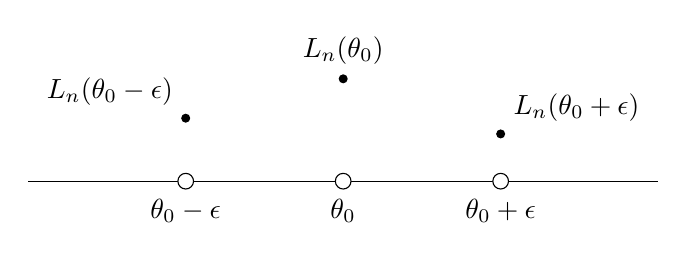
\begin{tikzpicture}
\draw (-4,0) -- (4,0);
\node[fill=white, circle, draw, inner sep=2pt, label=below:$\theta_0 - \epsilon$] at (-2, 0) {};
\node[fill=white, circle, draw, inner sep=2pt, label=below:$\theta_0$] at (0, 0) {};
\node[fill=white, circle, draw, inner sep=2pt, label=below:$\theta_0 +\epsilon$] at (2, 0) {};

\node[fill=black, circle, draw, inner sep=1pt, label=above left:$L_n(\theta_0 - \epsilon)$] (A) at (-2, 0.8) {};
\node[fill=black, circle, draw, inner sep=1pt, label=above:$L_n(\theta_0)$] (B) at (0, 1.3) {};
\node[fill=black, circle, draw, inner sep=1pt, label=above right:$L_n(\theta_0 +\epsilon)$] (C) at (2, 0.6) {};
\end{tikzpicture}
\end{center}

Cogemos entonces un conjunto $S_n$ definido de la siguiente forma:

\begin{align*}
S_n = \{ (x_1,\dotsc,x_n) &\tq L_n(\theta_0;x_1, \dotsc,x_n) > L_n(\theta_0 - \epsilon; x_1, \dotsc, x_n) \\
&\y  L_n(\theta_0;x_1, \dotsc,x_n) > L_n(\theta_0 + \epsilon; x_1, \dotsc, x_n) \}
\end{align*}

Aplicando el teorema MV1 (\ref{thmMV}), tenemos que $\mathbb{P}_{\theta_0}(S_n) \convs 1$.

En algún punto del interior del intervalo $\Omega$ hay un máximo local. Como puede haber varios máximos locales, tomo $\hat\theta_n$ como el punto de máximo local más cercano a $\theta_0$.

Se cumple que cada uno de esos puntos de máximo satisfacen la ecuación de verosimilitud (\ref{eqMV2}). En consecuencia $\hat\theta_n$ satisface también esa misma ecuación. Por lo tanto

\[ \prob{\abs{\hat\theta_n - \theta_0} < \epsilon} \convs 1 \dimplies \prob{\abs{\hat\theta_n - \theta_0} \geq \epsilon} \convs 0 \]

y entonces

\[ \hat\theta_n \convprob \theta_0 \]
\end{proof}

\subsubsection{Información de Fisher}

Supongamos el conjunto de todos los estimadores de un parámetro $\theta$. Su error cuadrático medio es

\[ \ECM(\hat\theta) = \var{\hat\theta} + \sesgo^2(\hat\theta) \]

Si queremos buscar el \textit{mejor} estimador, buscamos los que minimicen el ECM. Por lo tanto, nos interesaremos en el subconjunto de estimadores insesgados ($\sesgo \hat\theta = 0$). Sin embargo, no tenemos una forma clara de distinguir cuál es mejor entre esos estimadores insesgados. En esta sección vamos a buscar una \textit{escala}, a la que llamaremos la \textbf{información de Fisher}, que nos dará una cota para la varianza de un estimador.

Suponemos que en la integral $\int f(x;\theta)\,dx$ se puede derivar dos veces bajo el signo integral (esto es, que $\int \frac{\partial^2}{\partial\theta^2} f(x;\theta)\,dx$ existe) y que además se puede permutar la integral y la derivada parcial (vemos condiciones suficientes en el apéndice \ref{secConds}, página \pageref{secConds}). Entonces

\[ \int f(x;\theta)\, dx = 1 \implies \dpa{}{\theta} \int f(x;\theta)\,dx = 0 \]

Por tanto

\[ \int \dpa{}{\theta}(\log f(x;\theta) ) f(x;\theta) \, dx = \mathbb{E}_\theta\left(\dpa{}{\theta}\log f(X;\theta)\right) = 0 \]

Si derivamos de nuevo en la integral

\begin{gather*}
\frac{\partial^2}{\partial\theta^2} \int f(x;\theta)\,dx = 0  = \int \frac{\partial^2}{\partial\theta^2} f(x;\theta)\,dx = \\
=\int \frac{\partial^2}{\partial\theta^2} \log f(x;\theta) f(x;\theta)\,dx + \int\dpa{}{\theta} \log f(x;\theta) \cdot \dpa{}{\theta}f(x;\theta)\,dx = \wtf \\
=\int \frac{\partial^2}{\partial\theta^2}\log f(x;\theta) f(x;\theta)\, dx + \int \left(\dpa{}{\theta}\log f(x;\theta)\right)^2 f(x;\theta)\,dx = \\
= \mathbb{E}_\theta \left[\frac{\partial^2}{\partial\theta^2}\log f(X;\theta) \right]
	+ \mathbb{E}_\theta \left[ \left(\dpa{}{\theta} \log f(X;\theta)\right)^2\right] = 0
\end{gather*}

\noindent El segundo valor se llama información de Fisher:

\begin{defn}[Información\IS de Fisher] Se denota por $I(\theta)$ la información de Fisher del parámetro $\theta$

\[ I(\theta) =\esp[\theta]{-\frac{\partial^2}{\partial\theta^2} \log f(X;\theta)} =\esp[\theta]{\left(\dpa{}{\theta} \log f(X;\theta)\right)^2} \]

Representa intuitivamente la \textit{cantidad de información} acerca del valor del parámetro $\theta$ contenida en una observación de $X$.
\end{defn}

¿En qué consiste esa cantidad de información? Tomemos, por ejemplo, una normal $N(0,\theta)$ con $\theta$ pequeña. Una observación $X$ que hagamos nos dará mucha información sobre el modelo, ya que todos los valores de la normal están muy agrupados, y por lo tanto $I(\theta)$ será grande. Si tomamos $\theta$ grande, una observación $X$ no nos dará mucha información sobre el modelo porque los valores están más dispersos, y por lo tanto tendremos un valor de $I(\theta)$ pequeño.

La información de Fisher nos da una cota inferior para la varianza.

\begin{theorem}[Cota\IS de Fréchet-Cramér-Rao] Dado $\hat\theta$ un estimador insesgado de $\theta$, entonces
\label{thmCotaFCR}
\[ \var{\hat\theta} \geq \frac{1}{nI(\theta)} \]

donde $\frac{1}{nI(\theta)}$ se llama la \textbf{cota de Fréchet-Cramér-Rao}.
\end{theorem}

\begin{proof} Tomamos la v.a. $Z$ como la derivada del logaritmo de la verosimilitud

\[ Z = \dpa{}{\theta}\log L_n (X,\theta) = \sum_{i=1}^n \dpa{}{\theta} \log f(X_i;\theta) \]

La desigualdad de Cauchy-Schwartz establece que \footnote{Por ejemplo, porque no tengo ni idea de dónde sale esto.}

\[ \var[\theta]{T_n} \geq \frac{\text{Cov}_\theta^2 (Z,T_n)}{\var[\theta]{Z}} \]

Veremos que el numerador vale 1 si $T_n$ es un estimador insesgado, y que $\var[\theta]{Z} = n I(\theta)$.

Primero observamos que

\[ \esp[\theta]{Z} = \sum_{i=1}^n \esp{\frac{\partial}{\partial\theta} \log f(X_i;\theta)} = 0 \]

Y la varianza

\[ \var[\theta]{Z} = \sum_{i=1}^n \var[\theta]{\frac{\partial}{\partial\theta} \log f(X_i;\theta)} = \sum_{i=1}^n \esp{\left(\dpa{}{\theta} \log f(X;\theta)\right)^2}[\theta] = n I(\theta) \]

La primera parte está demostrada.

Ahora vemos que, si $\esp[\theta]{Z} = 0$, entonces

\[ \text{Cov }(Z,T_n) = \esp[\theta]{ZT_n} - \underbrace{\esp[\theta]{Z}}_0 \esp[\theta]{T_n} = \esp[\theta]{ZT_n}  \]

Como $Z$ y $T_n$ dependen de la muestra

\[ \esp[\theta]{ZT_n} = \esp[\theta] {Z(X_1,\dotsc,X_n) \cdot T_n(X_1,\dotsc,X_n)}= \int_{\real^n} Z(x_1,\dotsc,x_n) \cdot T_n(x_1,\dotsc,x_n) \cdot f_\theta(x_1,\dotsc,x_n)\,d(x_1, \dotsc, x_n) \]

Como las $X_1,\dotsc,X_n$ son independientes,

\[ f_\theta(x_1,\dotsc,x_n) = \prod_{i=1}^nf(x_i;\theta)\ \]

y la integral nos queda entonces como una serie de integrales iteradas

\[ \int_\real \dotsb \int_\real Z(x_1,\dotsc,x_n) \cdot T_n(x_1,\dotsc,x_n)  \prod_{i=1}^nf(x_i;\theta)\,dx_i \]

Vemos cuánto vale $Z$:

\[ Z = \dpa{}{\theta}\log f(x_i;\theta) = \sum_{i=1}^n \frac{\dpa{}{\theta}f(x_i;\theta)}{f(x_i;\theta)} \]

Pero

\[ \sum_{i=1}^n \frac{\dpa{}{\theta}f(x_i;\theta)}{f(x_i;\theta)}  \prod_{i=1}^nf(x_i;\theta)\,dx_i  = \sum_{i=1}^n\left[ \dpa{}{\theta}f(x_i;\theta \cdot \prod_{\substack{j=1\\j\neq i}}^n f(x_j;\theta) \right] \]

que por la regla de la cadena es igual a

\[ \dpa{}{\theta}\left[\prod_{i=1}^n f(x_i;\theta) \right] \]

y entonces nos queda que

\begin{gather*}
\cov (Z,T_n) = \esp[\theta]{ZT_n} = \int_\real \dotsc \int_\real T_n(x_1,\dotsc,x_n) \dpa{}{\theta} \prod_{i=1}^n f(x_i;\theta)\, dx_i = \\
 = \dpa{}{\theta} \int_\real \dotsc \int_\real T_n(x_1,\dotsc,x_n) \prod_{i=1}^n f(x_i;\theta)\, dx_i =\\
 = \dpa{}{\theta} \esp[\theta]{T_n}
 \end{gather*}

Como $T_n$ es un estimador insesgado $\esp[\theta]{T_n}  = \theta$ y entonces $\text{Cov}\,(Z,T_n) = 1$. Por lo tanto, nos queda que

\[ \var{\hat\theta} \geq \frac{1}{nI(\theta)} \]

Además, si $T_n$ no fuese un estimador insesgado

\[ \var{\hat\theta} \geq \frac{\left(dpa{}{\theta} \esp[\theta]{T_n} \right)^2}{n I(\theta)} \]

y por lo tanto

\[ \text{ECM}(T_n) \geq \frac{\left(\dpa{}{\theta} \esp[\theta]{T_n}\right)^2}{n I(\theta)} + \text{Sesgo }^2 (T_n) \]
\end{proof}

\begin{defn}[Estimador\IS eficiente]
Se dice que un estimador es eficiente si su varianza es igual a la cota de Fréchet-Cramér-Rao (\ref{thmCotaFCR}), es decir
\[ \var{\hat\theta} = \frac{1}{nI(\theta)} \]
\end{defn}

\vspace{-10mm} % increíble la cantidad de espacio que se pierde sin esta línea
\subsubsection{Eficiencia asintótica}
\begin{theorem}[Teorema\IS MV3] Supongamos que se verifican las condiciones MV0 - MV3 (ver teoremas \ref{thmMV}, \ref{thmMV2}) y además:

\subparagraph{MV4)} La integral $\int f(x;\theta)\,dx$ se puede derivar dos veces bajo el signo integral.
\subparagraph{MV5)} Para cada $x$ la densidad $f(x;\theta)$ es tres veces diferenciable con respecto a $\theta$, con la tercera derivada continua en $\theta$.
\subparagraph{MV6)} La información de Fisher es estrictamente positiva y finita: $0 < I(\theta_0) < \infty$
\subparagraph{MV7)} Para cada $\theta_0\in \Theta$ existen un número $c > 0$ y una función $M(x)$, que pueden depender de $\theta_0$, tales que \[ \esp[\theta_0]{M(X)} < \infty \] y \[ \abs{\frac{\partial^3\log f}{\partial\theta^3}(x;\theta)} \leq M(x)\; \forall x;\;\forall\theta \in (\theta_0 - c,\theta_0 + c) \]

Entonces, si $\hat{\theta}_n(\sample)$ es cualquier sucesión consistente de soluciones de las ecuaciones de verosimilitud, se verifica

\[ \sqrt{n}\left(\hat{\theta}_n-\theta_0\right) \convdist N\left(0,\frac{1}{\sqrt{I(\theta_0)}}\right) \]

\end{theorem}

\begin{proof}

\begin{gather}
 \tilde\Psi_n(\theta) = L_n  \\
 \tilde\Psi_n' = \dpa{\Psi_n(\theta)}{\theta} \label{eqT3_2} \\
 f' = \dpa{f}{\theta}f
 \end{gather}

 donde la función \ref{eqT3_2} se llama el \textbf{score} (quizás).

 Recordemos que $\hat\Psi_n(\theta)$ depende de la muestra. Para cada muestra fija se tiene

 \[ \tilde\Psi_n(\hat\theta_n) = \hat\Psi_n'(\theta_0) + (\hat\theta_n-\theta_0)\Psi_n''(\theta_0) + \frac{\left(\hat\theta_n-\theta_0\right)^2}{2}\tilde\Psi_n'''(\theta_n^\ast) \]

Para algún $\theta_n^\ast$ entre $\hat\theta_ n$ y $\theta_0$. Como el primer miembro es 0, resulta

\[ \sqrt{n}\left(\hat\theta_n-\theta_0\right) = \frac{\frac{1}{\sqrt{n}}\tilde\Psi_n'(\theta)^2}{-\frac{1}{n}\Psi_n''(\theta_0) - \frac{1}{2n}\left(\hat\theta_n-\theta_0\right)\tilde\Psi_n'''(\theta_n^\ast)} \]

Vamos a demostrar que esto converge en tres pasos:

\begin{itemize}
\item Numerador converge a $N(0,\sqrt{I(\theta_0)})$.
\item Primera parte converge a $I(\theta_0)$.
\item Segunda parte denom. converge a 0 en prob.
\end{itemize}

Tendremos por lo tanto que

\[ \sqrt{n}\left(\hat\theta_n-\theta_0\right) \convdist \frac{N(0, \sqrt{I(\theta_0)}}{I(\theta_0)+0} \]

Y usando la tercera condición del teorema de Slutsky (\ref{thmSlutsky}), tendremos que

\[  \frac{N(0, \sqrt{I(\theta_0)}}{I(\theta_0)+0}  \convdist N\left(0,\frac{1}{\sqrt{I(\theta_0)}}\right) \]

\paragraph{Parte 1: Numerador}

\[ \frac{1}{\sqrt{n}}\tilde\Psi_n'(\theta_0) = \frac{\sqrt{n}}{n}\sum_{i=1}^n \left[\frac{f'(X_i;\theta_0)}{f(X_i;\theta_0)} - \esp[\theta_0]{\frac{f'(X_i;\theta_0)}{f(X_i;\theta_0)}}\right] \]

Como $\esp[\theta_0]{\frac{f'(X_i;\theta_0)}{f(X_i;\theta_0)}} = 0$ (vete tú a saber por qué), la aplicación del TCL (\ref{thmCentral}) a las variables $Y_i = \frac{f'(X_i;\theta_0)}{f(X_i;\theta_0)}$ y la definición de $I(\theta_0)$ proporcionan directamente

\[ \frac{1}{\sqrt{n}}\hat\Psi_n'(\theta_0) \convdist N(0,\sqrt{\var{Y}}) \]

Calculamos ahora esa desviación típica:

\begin{gather*}
 \var[\theta]{Y} = \esp[\theta]{Y^2} - \esp[\theta]{Y}^2 = \esp[\theta]{Y^2} = \\
 = \esp[\theta]{\left(\dpa{}{\theta}\log f(X;\theta)\right)^2} = I(\theta)
\end{gather*}

Y por lo tanto nos queda que

\[ \frac{1}{\sqrt{n}}\hat\Psi_n'(\theta_0) \convdist N\left(0,\sqrt{I(\theta_0)}\right) \]

\paragraph{Parte 2: Denominador A}

Operamos con

\[ -\frac{1}{n}\Psi_n''(\theta_0) \]

Si derivamos de nuevo $\tilde\Psi_n''$ con respecto a $\theta$ tenemos que

\[ \tilde\Psi_n''(\theta) = \sum_{i=1}^n \frac{f''(x_i;\theta)f(x_i;\theta) - \left(f'(x_i;\theta)\right)^2}{f^2(x_i;\theta)} \]

Entonces $\frac{1}{n}\Psi_n''(\theta_0)$ es un promedio, y por la LGN (\ref{thmGrandes})

\begin{align*}
- \frac{1}{n}\Psi_n''(\theta_0) & \convprob - \esp[\theta_0]{\frac{f''(x_i;\theta)f(x_i;\theta) - \left(f'(x_i;\theta)\right)^2}{f^2(x_i;\theta)}} =\\ & =\underbrace{\esp[\theta_0]{\left(\frac{f'(X_i;\theta_0)}{f(X_i;\theta_0)}\right)^2}}_{I(\theta_0)}- \esp[\theta_0]{\frac{f''(X_i;\theta_0)}{f(X_i;\theta_0)}}
\end{align*}

Operamos ahora con la segunda parte

\begin{gather*}
\esp[\theta_0]{\frac{f''(X_i;\theta_0)}{f(X_i;\theta_0)}} = \int_\real \frac{f''(X_i;\theta_0)}{f(X_i;\theta_0)}f(X_i;\theta_0)\,dx = \\
= \int_\real \left.\frac{\partial^2}{\partial\theta^2}f(x;\theta)\right|_{\theta=\theta_0}\,dx
\end{gather*}

y como según el enunciado del teorema podemos permutar la derivada con la integral dos veces, tenemos que

\[ \int_\real \left.\frac{\partial^2}{\partial\theta^2}f(x;\theta)\right|_{\theta=\theta_0}\,dx =  \left.\frac{\partial^2}{\partial\theta^2}\int_\real f(x;\theta)\,dx\right|_{\theta=\theta_0} = \left.\frac{\partial^2}{\partial\theta^2}0\right|_{\theta=\theta_0}  = 0 \]

Por lo tanto

\[ - \frac{1}{n}\Psi_n''(\theta_0) \convprob I(\theta_0) \]

\paragraph{Paso 3: Segunda parte del denominador}

\[\frac{1}{2n}\left(\hat\theta_n-\theta_0\right)\tilde\Psi_n'''(\theta_n^\ast) \convprob 0 \]

Por hipótesis del teorema, $\hat\theta_n$ se considera consistente y entonces \[ \left(\hat\theta_n-\theta_0\right) \convs 0 \] Analizaremos ahora la segunda parte de esa ecuación, $\tilde\Psi_n'''(\theta_n^\ast)$, y demostraremos que tiende a una constante.

\[ \tilde\Psi_n'''(\theta_n^\ast) = \frac{1}{n}\sum_{i=1}^n \frac{\partial^3}{\partial\theta^3}\log f(X_i;\theta) \]

Como $\hat\theta_n$ es consistente, $\theta_n^\ast$, que es un punto intermedio entre $\hat\theta_n$ y $\theta_0$, también tiende a $\theta_0$ en probabilidad. Entonces podemos aplicar la hipótesis MV7 del teorema y acotar la derivada parcial:

\[ \abs{\frac{\partial^3}{\partial\theta^3}\log f(X_i;\theta)} \leq M(X_i) \]

y por lo tanto podemos acotar en probabilidad

\[ \abs{\tilde\Psi_n'''(\theta_n^\ast)} < \frac{1}{n}\sum_{i=1}^n M(X_i) \]

Este término converge a una constante por lo tanto, y entonces se cumple que

\[\frac{1}{2n}\left(\hat\theta_n-\theta_0\right)\tilde\Psi_n'''(\theta_n^\ast) \convprob 0 \]
\end{proof}

\pagebreak
\subsection{Método de los momentos}
\index{Estimador!por el método de los momentos}
Sea $X\sim f(x;\theta)$, donde $\theta = (\theta_1,\dotsc,\theta_p)$ es un parámetro p-dimensional, con $p\geq1$.

Si los momentos $\alpha_k(\theta) = \esp[\theta_0]{X^k},\;k=1,\dotsc,p$ son funciones sencillas de los $\theta_i$, un procedimiento natural para obtener un estimador de $\theta$ es resolver en $\theta_1,\dotsc,\theta_p$ el sistema de ecuaciones

\begin{gather*}
m_1 = \alpha_1(\theta) \\
\dotsb \\
m_p = \alpha_p(\theta)
\end{gather*}

donde cada $m_k$ es el momento muestral:

\[ m_k = \frac{1}{n}\sum\limits_{i=1}^n X_i^k \]

La idea es estimar el parámetro de tal forma que los momentos muestrales coincidan con los momentos poblacionales. Por la LGN, cuando $n\to\infty$ entonces $m_k \to \alpha_k(\theta_0)$.

El método de los momentos se utiliza poco ya que da peores estimadores que el EMV. Sin embargo, puede resultar muy útil en casos en los que el EMV se calcula difícilmente o directamente no se puede calcular. Ahí hay que usar métodos numéricos de aproximación, y usando el método de los momentos podemos encontrar una primera aproximación que mejore la convergencia de los algoritmos numéricos de búsqueda de raíces.

\subsubsection{Ejemplos}

Si se tiene el modelo \[f(x;\theta) = \frac{1+\theta x}{2}\ind_{[-1,1](x)}\,\theta\in[-1,1] \] no es sencillo calcular el EMV pero sí obtener el estimador por el método de los momentos:

\[ \esp[\theta]{X} = \int_{-1}^1 x f(x;\theta)\,dx = \frac{\theta}{3} \]

Por tanto, la solución de $\avg{X} = \esp[\theta]{X}$ es $\tilde\theta_n = 3\avg{X}$, cuya varianza es

\[ \var[\theta]{\tilde\theta_n} = \var[\theta]{3\avg{X}} = 9\frac{\sigma^2}{n} = \frac{3-\theta^2}{n} \]

ya que \[ \sigma^2 = \var[\theta]{X}= \esp[\theta]{X^2} - \esp[\theta]{X}^2 = \frac{1}{3}-\frac{\theta^2}{9} \] Este estimador es consistente ya que, por la LGN, $3\avg{X} \convs 3\esp[\theta]{X}$.

Supongamos un ejemplo más complicado: $X\sim Beta(a,b)$.

\[ f(x;a,b) = \frac{\Gamma(a+b)}{\Gamma(a)\Gamma(b)} x^{a-1}(1-x)^{b-1} \ind_{[0,1]}(x) \]

y

\begin{align*}
\esp[\theta]{X} &= \int_0^1\frac{\Gamma(a+b)}{\Gamma(a)\Gamma(b)} x^{a}(1-x)^{b-1}\,dx = \\
&= \frac{\Gamma(a+b)}{\Gamma(a)}\frac{\Gamma(a+1)}{\Gamma(a+b+1)}\underbrace{\int_0^1\frac{\Gamma(a+b+1)}{\Gamma(a+1)\Gamma(b)} x^{a}(1-x)^{b-1}\,dx}_{=1 \text{ (f. densidad)}} =
\end{align*}

Sabiendo que $\Gamma(p+1) = p\Gamma(p)$

\[ \frac{\Gamma(a+b)}{\Gamma(a)}\frac{\Gamma(a+1)}{\Gamma(a+b+1)} =
	\frac{\Gamma(a+b)}{\Gamma(a)}\frac{a\Gamma(a)}{(a+b)\Gamma(a+b)} = \frac{a}{a+b} \]

y los estimadores quedan como

\begin{gather*}
\hat{a} = \avg{X}\left(\frac{\avg{X}(1-\avg{X})}{s^2}-1\right) \\
\hat{b} = (1-\avg{X})\left(\frac{\avg{X}(1-\avg{X})}{s^2}-1\right)
\end{gather*}

\subsection{Metodología bayesiana}
\index{Distribución!a priori}

En muchos casos se tiene cierta información a priori, antes de extraer la muestra, sobre la probabilidad de los diferentes valores del parámetro $\theta$. En estos casos se sabe, o se supone, que ciertos intervalos de valores de $\theta$ son \textit{más probables que otros} y se concreta esta información en una \textbf{distribución a priori sobre $\theta$} cuya función de densidad se denota $\pi(\theta)$.

De manera formal, la estadística bayesiana considera que el parámetro es una variable aleatoria y que la información previa se puede expresar a través de la distribución a priori del parámetro.

Entonces, si antes teníamos una v.a. $X\sim f(x;\theta)$, ahora lo que diremos es que $X$ sigue una distribución condicionada por un parámetro: $X\sim f(x|\theta)$.

En este caso, la muestra $X_1,\dotsc,X_n$ contiene información de la muestra y también de nuestro parámetro. Es decir, que podemos considerar la función de distribución de la muestra como \[ \prod_{i=1}^n f(x_i|\theta) \] Para juntar toda esta información usaremos el Teorema de Bayes:

\begin{theorem}[Teorema\IS de Bayes] Sea $A_1,A_2,\dotsc$ una partición del espacio muestral y sea $B$ un suceso cualquiera. Entonces

\[ \prob{A_i|B} = \frac{\prob{A_i\cap B}}{\prob{B}} = \frac{\prob{B|A_i}\cdot \prob{A_i}}{\sum_j \prob{B|A_j}\cdot \prob{A_j}} \]

Esta formulación se refiere a sucesos probabilísticos. Podemos reformularla con la información a priori del parámetro:

\begin{equation}
\label{eqBayes}
 \pi(\theta | x_1,\dotsc,x_n) = \frac{f(x_1,\dotsc,x_n|\theta)\pi(\theta)}{\displaystyle \int_\Theta f(x_1,\dotsc,x_n|\tau)\pi(\tau)\,d\tau}
 \end{equation}

donde $\Theta$ es todo el espacio paramétrico. A $ \pi(\theta | x_1,\dotsc,x_n) $ se le denomina \textbf{distribución a posteriori}\index{Distribución!a posteriori}
\end{theorem}

Como $\pi$ es una función de distribución, tenemos que

\[ \int_\Theta \pi(\theta|x_1,\dotsc,x_n)\,d\theta = 1 \]

para toda posible muestra $(x_1,\dotsc,x_n)$. Estudiaremos entonces la siguiente integral

\[ \int_\Theta \frac{f(x_1,\dotsc,x_n|\theta)\pi(\theta)}{\displaystyle \int_\Theta f(x_1,\dotsc,x_n|\tau)\pi(\tau)\,d\tau} \]

En esta, integral, el término

\[ \int_\Theta f(x_1,\dotsc,x_n|\tau)\pi(\tau)\,d\tau \]

es constante. Por lo tanto, lo que nos interesará será el numerador, la integral

\[ \int_\Theta f(x_1,\dotsc,x_n|\theta)\pi(\theta)\,d\theta \]

que nos dará la información que necesitamos.

\begin{defn}[Estimador\IS Bayes] Se define, para cada muestra dada $(x_1,\dotsc,x_n)$ como la esperanza de la distribución a posteriori:

\[ T_n(x_1,\dotsc,x_n) = \int_\Theta \theta\pi(\theta|x_1,\dotsc,x_n)\,d\theta \]
\end{defn}


\subsubsection{Ejemplos}

La estadística bayesiana se suele usar para estimar los votantes de un partido político. Por ejemplo, sea $\theta$ la proporción de votantes de un partido $P$, y sea $X$ la v.a. Bernoulli que toma valor 1 cuando un votante elige $P$ y 0 en otro caso. Es decir

\[ \begin{cases}
f(x|\theta) = \theta &\text{si } x=1 \\
f(x|\theta) = 1 - \theta &\text{si } x=0 \\
\end{cases} \]

Entonces tenemos que \[ f(x_1,\dotsc,x_n|\theta) = \prod_{i=1}^n f(x_i|\theta) = \theta^{\sum_{i=1}^n x_i} (1-\theta)^{n -\sum_{i=1}^n x_i} \]

Suponemos que la distribución a priori es una Beta(4,10):

\[ \pi(\theta) = \frac{\Gamma(14)}{\Gamma(4)\Gamma(10)}\theta^3(1-\theta)^9\ind_{[0,1]}(\theta) \]

Así pues, aplicando la fórmula de Bayes (\ref{eqBayes}) nos queda

\begin{equation}\label{eqE1}
\theta^{\sum x_i}(1-\theta)^{n-\sum x_i} \theta^3 (1-\theta)^9 = \theta^{3+\sum x_i} (1-\theta)^{ 9 + n - \sum x_i}
\end{equation} y entonces

\[  \pi(\theta | x_1,\dotsc,x_n)  \sim Beta(4 + \sum x_i, 10 + n - \sum x_i) \]

El estimador Bayes es, por lo tanto

\[ T_n = \frac{4 + \sum x_i}{14 + n} = \underbrace{\frac{n}{4 + 10 + n}\avg{x}}_{(A)} + \underbrace{\frac{4+10}{4+10+n}\frac{4}{4+10}}_{(B)} \]

Es decir, pondera las dos información que teníamos: la media de la distribución a priori $(B)$ y la media muestral $(A)$. Si nos fijamos en la expresión, si tenemos un tamaño muestral muy grande ($n\to\infty$) damos mucho más peso a la información de la muestra que a la distribución a priori. Sin embargo, si tenemos menos muestras nuestra distribución a priori influirá más en el resultado.

Con los datos $\sum x_i = 125$ y $n = 1000$, el estimador Bayes toma valor $0.127$, mientras que el e.m.v. valdría $0.125$. Es decir, nuestro estimador bayesiano pondera la información que teníamos previamente y considera que en nuestra distribución a priori era más probable valores más altos.

Curiosamente, en (\ref{eqE1}) hemos pasado de una distribución a priori a una distribución a posteriori fácilmente identificable con una distribución Beta. Esto tiene que ver con el concepto de familias conjugadas.

\subsubsection{Familias conjugadas}

\begin{defn}[Familia\IS conjugada] Sea $\mathcal{F}$ una familia de distribuciones paramétricas $f(\cdot | \theta),\;\theta\in\Theta$; y sea $\Pi$ una familia de distribuciones a priori $\pi(\theta)$ sobre el parámetro $\theta$.

Diremos que $\Pi$ es la familia de dsitribuciones a priori conjugada de $\mathcal{F}$ si la distribución a posteriori $ \pi(\theta | x_1,\dotsc,x_n) $ también pertence a $\Pi$ para toda muestra $ ( x_1,\dotsc,x_n) $ y para toda a priori de $\Pi$.
\end{defn}

Tenemos varias familias conjugadas identificadas:
\begin{table}[hbtp]
\centering
\begin{tabular}{|c|c|}
\hline
$\mathcal{F}$ & $\Pi$ \\
\hline
Binomial & Beta \\
\hline
Normal & Normal \\
\hline
\end{tabular}
\caption{Familias conjugadas}
\end{table}

\section{Estimación por intervalos de confianza}
\label{secConfianza}
Al igual que en el tema anterior, vamos a obtener información sobre un parámetro desconocido $\theta\in\Theta$ a partir de una muestra $X_1,…,X_n$. Habíamos logrado una estimación puntual, pero, ¿por qué va a ser válido sólo ese valor? ¿Podría ser válido un valor cercano al estimador?

Este tema responde a esa pregunta: ofrece un intervalo que típicamente contiene a un estimador puntual, de posibles valores para un parámetro. Veremos cómo construir ese intervalo y la información que ofrecen.

\begin{defn}[Intervalo\IS de confianza] Sea una muestra $X_1,…,X_n$ de una v.a. con una función de distribución $F(.;\theta)$, con $\theta\in\Theta⊂\real$ un parámetro desconocido. Sean dos estadísticos $T_n^{(1)}(X_1,…,X_n)$ y $T_n^{(2)}(X_1,…,X_n)$ con $T_n^{(1)} < T_n^{(2)}$ y un valor $\alpha\in(0,1)$. Supongamos que se verifica

\[ \prob[\theta]{T_n^{(1)}(\sample ) < \theta < T_n^{(2)}(\sample) } = 1-\alpha\; \forall\theta\]

Entonces para una realización concreta de la muestra $\sample[x]$ se dice que el intervalo $(T_n^{(1)}(\sample[x]) ,T_{n}^{(2)}(\sample[x]))$ es un intervalo de confianza para $\theta$ con nivel de confianza $1-\alpha$ y lo denotaremos como

\[ IC_{1-\alpha}(\theta) \]
\end{defn}

Probemos esta definición con una muestra $\sample$ de v.a.i.i.d. $N(\mu,\sigma)$ donde $\mu$ es un parámetro desconocido y $\sigma$ es conocida. Se sabe que

\[ \avg{X} \sim N\left(\mu,\frac{\sigma}{\sqrt{n}}\right) \]

y, tipificando,

\[ \frac{\avg{X}-\mu}{\frac{\sigma}{\sqrt{n}}} \sim~ N(0,1) \]

Por tanto, si para cualquier $\alpha\in(0,1)$, $z_\alpha$ denota el cuantil $1-\alpha$ en la normal estándar ($Φ(z_\alpha) = 1-\alpha$, siendo $Φ$ la función de distribución de la $N(0,1)$) tenemos

\[ \prob[\mu]{-z_{\alpha/2} < \frac{\avg{X}-\mu}{\frac{\sigma}{\sqrt{n}}}  < z_{\alpha/2}} = 1-\alpha \]

y, despejando

\[ \prob[\mu]{\avg{X} - z_{\alpha/2}\frac{\sigma}{\sqrt{n}} < \mu < \avg{X} + z_{\alpha/2}\frac{\sigma}{\sqrt{n}}} = 1-\alpha \]

Y por lo tanto, el intervalo

\[ \left(\avg{x} - z_{\alpha/2}\frac{\sigma}{\sqrt{n}}, \avg{x} + z_{\alpha/2}\frac{\sigma}{\sqrt{n}}\right)\]

es un \textbf{intervalo de confianza de nivel $1-\alpha$ para $\mu$}.

Intuitivamente y en términos frecuentistas, si por ejemplo $1-\alpha = 0.95$ y extraemos muchas muestras de una $N(0,1)$ aproximadamente en el 95\% de los casos el intervalo contendrá el verdadero valor de $\mu$.

\subsection{Intervalos de confianza asintóticos basados en el TCL}

Si $X$ no es normal, sabemos que si $\mu$ y $\sigma$ son finitas, encontes $\avg{X} \sim N\left(\mu,\frac{\sigma}{\sqrt{n}}\right)$ por el TCL (\ref{thmCentral}). Entonces

\[ 1-\alpha = \simeq \prob{-z_{\alpha/2} \leq \frac{\avg{X} - \mu}{\frac{\sigma}{\sqrt{n}}} \leq z_{\alpha/2}} \]

Es decir, obtenemos un intervalo de confianza aproximado si el tamaño de la muestra es grande.

\paragraph{Aplicación: Intervalo de confianza aproximado para una proporción $p$} Sean $\sample$ i.i.d. Bernoulli($p$). Por el TCL

\[ \frac{\avg{X}-p}{\sqrt{\frac{p(1-p)}{n}}} \sim N(0,1) \]

y reemplazando $p$ por su estimador natural $\hat{p} = \avg{X}$ obtenemos que el intervalo de confianza aproximado para $p$ es

\[ \left( \avg{x} - z_{\alpha/2} \sqrt{\frac{\avg{x}(1-\avg{x})}{n}}, \avg{x} + z_{\alpha/2} \sqrt{\frac{\avg{x}(1-\avg{x}}{n}} \right) \]

\subsection{Método de la cantidad pivotal}
\index{Cantidad!pivotal}
Una metodología general para obtener un intervalo de confianza para $\theta$ consiste en encontrar una función $Q(\theta;\sample)$, llamada \textbf{cantidad pivotal} cuya distribución no dependa de $\theta$ y sea conocida, al menos de modo aproximado. A partir de esta distribución, fijado un valor $\alpha\in(0,1)$ se obtienen dos valores $q_1(\alpha), q_2(\alpha)$ tales que

\[ \prob[\theta]{q_1(\alpha) < Q(\theta;\sample) < q_2(\alpha)} = 1-\alpha \]

Despejando $\theta$ se obtiene una expresión del tipo

\[ \prob[\theta]{T_n^{(1)}(\sample) < T_n^{(2)}(X_1,\dotsc,X_n)} = 1- \alpha \]

\subsection{Construcción de intervalos de confianza habituales}

\subsubsection{Distribución $\chi^2$}
\index{Distribución!$\chi^2$}\label{ChiSquared}
Estamos interesados en obtener intervalos de confianza exactos, válidos para cualquier $n$, para $\sigma^2$ en una normal. Para ello presentaremos una distribución auxiliar que tiene una especial importancia en estadística, la \textbf{distribución $\chi_k^2$}, que en realidad es la distribución $Γ(\frac{1}{2}, \frac{k}{2})$.
Esta distribución surge del estudio de la distribución de las formas cuadráticas $X'AX$. En particular, si $\{Z_n\}$ son variables aleatorias normales estandarizadas, entonces
\[ \sum Z_k^2 \sim \chi^2 \]

De hecho, aplicando esto a una suma de varias v.a. $\sample$ $S^2$, nos queda que

\[ \frac{(n-1)S^2}{\sigma^2} \sim \chi^2_{n-1} \]

Este resultado proporciona directamente una cantidad pivotal y, en consecuencia, un intervalo de confianza de nivel $1-\alpha$ para $\sigma^2$:

\[ \left(
	 \frac{(n-1)s^2}{\chi^2_{n-1;\alpha/2}},\; \frac{(n-1)s^2}{\chi^2_{n-1;1-\alpha/2}}
\right) \]

\subsubsection{Distribución $t$ de Student}
\index{Distribución!$t$ de Student}
Sea $Z\sim N(0,1)$ y $W\sim \chi_k^2$. Supongamos que $Z$ y $W$ son independientes. Entonces la distribución de la v.a.

\[ T = \frac{Z}{\sqrt{W/k}} \]

se denomina distribución $t$ de Student con $k$ grados de libertad. Su forma se aproxima a una normal $N(0,1)$.

\begin{theorem}[Lema\IS de Fischer-Cochran] Si \sample son v.a.i.i.d. con distribución $N(\mu,\sigma)$ entonces $\avg{X}$ y $S^2$ (desviación) son estadísticos independientes.
\end{theorem}

Este teorema tiene una consecuencia importante, y es que podemos obtener un intervalo de confianza exacto para $\mu$ en $N(\mu,\sigma)$ aún cuando $\sigma$ es desconocida.

\subsection{Intervalos de confianza bayesianos}

En un problema de inferencia con un enfoque bayesiano, el elemento fundamental para realizar la inferencia es la distribución a posteriori $\pi(\theta|\sample[x])$. A partir de esa distribución se define una \textbf{región creíble}\index{Región!creíble} de nivel $1 - \alpha$ como un subconjunto $A \subseteq \Theta$ tal que

\[ \int_A π(\theta|\sample[x])\,d\theta = 1 - \alpha \]

\chapter{Contraste de hipótesis}

\section{Conceptos básicos}

El objetivo de la teoría de contraste de hipótesis es \textbf{elegir entre dos posibilidades excluyentes}, las hipótesis nula e alternativa, relativas al valor de un parámetro poblacional a partir de la información proporcionada por los datos muestrales.

Sea $\sample$ una muestra aleatoria de una v.a. $X$ con función de distribución $F_\theta$ donde $\theta \in \Theta$. Dada una partición del espacio paramétrico $\Theta=\Theta_0 \cup \Theta_1$, deseamos decidir, en base a la muestra obtenida, si $\theta$ está en $\Theta_0$ o en $\Theta_1$. En el primer caso se cumple la hipótesis nula, en el segundo la alternativa. Ambas hipótesis son excluyentes.

Para resolver el problema definiremos una región de rechazo. Esta región $R\subseteq\real^n$ nos permitirá valorar si el parámetro está en $\Theta_0$ o en $\Theta_1$ en base a la muestra obtenida. De esta forma, si $(\sample[x]) \in R$, se rechaza la hipótesis nula.

El paso más importante del contraste de hipótesis es construir la región de rechazo $R$, y a partir de entonces los pasos son muy mecánicos. En el apéndice \ref{secRegRechazo}, página \pageref{secRegRechazo}, tenemos varias muestras de regiones de rechazo.

En el test de hipótesis podemos cometer dos tipos de fallos:

\begin{itemize}
\item \textbf{Error de tipo I} Rechazar $H_0$ cuando $H_0$ es cierta.\label{errorTipoI}\index{Error!de tipo I}
\item \textbf{Error de tipo II} Aceptar $H_0$ cuando $H_0$ es falsa.\label{errorTipoII}\index{Error!de tipo II}
\end{itemize}

Para medir la probabilidad de cometer uno de esos fallos definimos la función de potencia

\begin{defn}[Función\IS de potencia] La función de potencia de un test con región de rechazo $R$ para contrastar $H_0: \theta \in \Theta_0$ frente a $H_1:\theta \in \Theta_1$ es la función

\begin{align*}
\appl{\beta_n}{\Theta&}{[0,1]} \\
\theta&\longmapsto \beta_n(\theta) = \prob[\theta]	{(\sample) \in R}
\end{align*}

y nos da la probabilidad de rechazar la hipótesis $\Theta_0$.\label{defFuncPotencia}
\end{defn}


\subsection{Teoría de Neyman-Pearson}
\label{secNeymanPearson}
Nos gustaría que $\beta_n(\Theta_0) = 0$ y que $\beta_n(\Theta_1) =1$, pero normalmente no pasará esto, sino que $\beta_n$ será una función continua y suave del parámetro.

La teoría de Neyman-Pearson trata de responder a este problema con los dos siguientes pasos:

\paragraph{Acotar la máxima probabilidad de error de tipo I}

\begin{itemize}
\item Se fija un \textbf{nivel de significación}\index{Nivel!de significación} $\alpha \in (0,1)$. Típicamente se toma $\alpha = 0.05$.
\item Se define el \textbf{tamaño de un test}\index{Tamaño!de un test} como la máxima probabilidad de error de tipo I, o como

\[ \max_{\theta \in \Theta_0} \prob[\theta]{R} = \max_{\theta \in \Theta} \beta_n(\theta) \]

\item Se busca una región de rechazo $R$ tal que \[ \max_{\theta \in \Theta_0} \prob[\theta]{R} \leq \alpha \]
\end{itemize}

Tal y como hemos definido $\alpha$, se puede considerar que el nivel de significación nos indica la probabilidad de cometer un error de tipo I, es decir, de rechazar $H_0$ cuando es cierta. Por lo tanto, cuanto menor es el nivel de significación más \textit{seguros} estamos de que no estamos rechazando $H_0$ por error.

\paragraph{Minimizar la probabilidad de error de tipo II}

Se intenta buscar una región de rechazo $R$ que maximice la función de potencia cuando $\theta \in \Theta_1$.

Aquí podemos ver por qué las dos hipótesis no son simétricas. Los tests de hipótesis están diseñados para controlar la probabilidad máxima de rechazar $H_0$ cuando es cierta. En consecuencia, suelen ser conservadores con la hipótesis nula: hace falta mucha evidencia muestral para rechazar $H_0$. Observemos que es posible que, con los mismos datos, $H_0$ se rechace para un nivel de significación $\alpha = 0.05$ y se acepte para $\alpha = 0.01$.

Además de la asimetría, tenemos que pensar que al aceptar $H_0$ no significa que la hayamos demostrado, sino simplemente que no se ha encontrado suficiente evidencia empírica a nivel prefijado $\alpha$ en contra de $H_0$. \textbf{No es una demostración matemática}.

\newpage
\section{Problema de una muestra}

En una primera aproximación, los problemas de contraste de hipótesis  pueden clasificarse en problemas de una muestra o de dos, según haya sólo una población de interés o queramos comparar dos poblaciones y dispongamos de una muestra de cada una de ellas. Presentaremos las ideas básicas en el caso de los problemas de una muestra pero pueden extenderse de modo análogo a los de dos muestras.

\paragraph{Dualidad con los intervalos de confianza}

En algunos casos de hipótesis nula simple, aparece una dualidad entre el contraste de hipótesis y los intervalos de confianza (\ref{secConfianza}). Si tenemos $H_0:\; \mu = \mu_0$, entonces aceptar $H_0$ significa que $\mu \in IC_{1 - \alpha}(\theta)$, es decir, que está en el intervalo de confianza. La región de rechazo sería entonces

\[ R = \{ (\sample[x])\tq \theta(\sample[x]) \notin IC_{1 - \alpha}(\theta) \} \]

\begin{defn}[p-valor del contraste] Se define el p-valor del contraste como el ínfimo de los niveles de significación $\alpha$ para los que se rechaza $H_0$.

De esta forma, si $\alpha$ es menor que el p-valor, aceptaremos $H_0$ y si es mayor, la rechazaremos.
\end{defn}

¿Qué información nos va a dar el p-valor? Supongamos que tenemos, por ejemplo, un \textbf{p-valor pequeño} ($ < 0.01$). Con este valor rechazaríamos la hipótesis nula para los valores más habituales de niveles de significación ($0.01, 0.05, 0.1$). Por lo tanto, en este caso \textbf{lo razonable sería rechazar $H_0$}.

Por otra parte, supongamos que tenemos un \textbf{p-valor grande} ($ > 0.1 $). En este caso, aceptaríamos la hipótesis nula para los valores más habituales de $\alpha$, y entonces \textbf{lo razonable sería aceptar $H_0$}.

Un p-valor que se encuentra entre 0.01 y 0.1 se considera \textbf{dudoso}. Lo razonable es revisar la muestra, y si es posible, aumentar su tamaño. \textbf{No se puede decidir} de manera razonable entre $H_0$ y $H_1$.

De forma general, el p-valor de contraste nos dice la probabilidad de observar la muestra que hemos obtenido suponiendo que $H_0$ es cierta. Si es muy bajo, nos indicará que es muy poco probable que la muestra obtenida haya salido así por pura casualidad.

\pagebreak
\subsection{Regiones de rechazo para contrastes habituales}
\subsubsection{Contraste de la media de una distribución}

En todo caso se rechaza $H_0$ cuando $(\sample) \in R$. Para hallar las regiones de rechazo buscaremos los \textbf{estadísticos de contraste}\index{Estadístico!de contraste}, medidas de lo razonable que es la hipótesis nula y que depende de la muestra obtenida. Cuando la hipótesis nula sea cierta, el estadístico del contraste estará en zonas de alta probabilidad.

\paragraph{Distribución normal con varianza conocida}

Primero construiremos el estadístico del contraste $Z$, que depende de la media muestral obtenida.

\[ Z = \frac{\avg{X}-\mu_0}{\sigma/\sqrt{n}} \]

Si $H_0:\;\mu=\mu_0$ es cierta entonces $Z\sim N(0,1)$. Entonces las regiones de rechazo son

\begin{table}[hbtp]
\centering
\begin{tabular}{|c|c|}
\hline  $H_0$ & $R$  \\
\hline  $\mu=\mu_0$ & $\{ (\sample[x]) \tq \abs{Z} \geq z_{\frac{\alpha}{2}}\}$ \\
\hline  $\mu\leq\mu_0$ & $\{ (\sample[x]) \tq Z \geq z_{\frac{\alpha}{2}}\}$ \\
\hline  $\mu\geq\mu_0$ & $\{  (\sample[x]) \tq Z \leq z_{\frac{\alpha}{2}}\}$ \\
\hline
\end{tabular}
\caption{Regiones de rechazo para una normal $N(\mu,\sigma)$.}
\end{table}

\paragraph{Distribución normal con varianza desconocida}

Sea $\sample$ una muestra aleatoria de $X\sim N(\mu,\sigma)$ con $\sigma$ desconocido. Entonces el estadístico del contraste sigue una distribución $T$ de Student de $n-1$ grados de libertad:

\[ T=\frac{\avg{X} - \mu_0}{s/\sqrt{n}} \]

\begin{table}[hbtp]
\centering
\begin{tabular}{|c|c|}
\hline  $H_0$ & $R$  \\
\hline  $\mu=\mu_0$ & $\{ (\sample[x]) \tq \abs{T} \geq t_{\frac{\alpha}{2}}\}$ \\
\hline  $\mu\leq\mu_0$ & $\{ (\sample[x]) \tq T \geq t_{\frac{\alpha}{2}}\}$ \\
\hline  $\mu\geq\mu_0$ & $\{  (\sample[x]) \tq T \leq t_{\frac{\alpha}{2}}\}$ \\
\hline
\end{tabular}
\caption{Regiones de rechazo para una normal $N(\mu,\sigma)$ con $\sigma$ desconocida.}
\end{table}

\pagebreak
\paragraph{Tests de nivel aproximado $\alpha$ (muestras grandes) para la media de cualquier distribución}

 Sea $\sample$ una muestra aleatoria de $X$ con $\esp{X} = \mu < \infty$. Entonces el estadístico del contraste es

 \[ Z= \frac{\avg{X}-\mu_0}{S/\sqrt{n}}\stackrel{TCL}{\sim} N(0,1) \]

 si $H_0:\, \mu=\mu_0$ es cierta. Por lo tanto, nos quedamos con las siguientes regiones:

\begin{table}[hbtp]
\centering
\begin{tabular}{|c|c|}
\hline  $H_0$ & $R$  \\
\hline  $\mu=\mu_0$ & $\{ (\sample[x]) \tq \abs{Z} \geq z_{\frac{\alpha}{2}}\}$ \\
\hline  $\mu\leq\mu_0$ & $\{ (\sample[x]) \tq Z \geq z_{\frac{\alpha}{2}}\}$ \\
\hline  $\mu\geq\mu_0$ & $\{  (\sample[x]) \tq Z \leq z_{\frac{\alpha}{2}}\}$ \\
\hline
\end{tabular}
\caption{Regiones de rechazo para la media de cualquier distribución}
\end{table}

\pagebreak[3]
\section{Contrastes para dos muestras}

Supongamos que tenemos 2 muestras $X_1,...,X_N$ y $Y_1,...,Y_N$. Siendo $\mu_1$ la esperanza de $X$ y $\mu_2$ la esperanza de $Y$.

Podemos plantear hipótesis del tipo
\begin{itemize}
\item $H_0: \,\,\, \mu_1=\mu_2$
\item $H_0: \,\,\, \mu_1\leq\mu_2$
\item $H_0: \,\,\, \sigma_1 = \sigma_2$
\end{itemize}
Este último caso (si las varianzas son iguales) suele ser un requisito previo antes de plantearte contrastes como el segundo ejemplo.

Uno de los test más usuales es el de igualdad de medias para dos poblaciones \textbf{homocedásticas} \index{Muestra!homocedástica}, es decir, con $\sigma_1=\sigma_2$.

Si \[\left.\begin{array}{cc}
X\sim N(\mu_1,\sigma)\\
Y\sim N(\mu_2,\sigma)
\end{array}\right\}\text{ Independientes } \begin{array}{cc}
\gor{X} -\mu_1 \sim N\left(0,\frac{\sigma}{\sqrt{n_1}}\right)\\
\gor{Y} - \mu_2 \sim N\left(0,\frac{\sigma}{\sqrt{n_2}}\right)
\end{array}\]
Entonces:
\[\frac{(\gor{X}-\mu_1) - (\gor{Y} - \mu_2)}{\sigma\sqrt{\frac{1}{n_1} + \frac{1}{n_2}}}\sim N(0,1)\]

Todo esto suponiendo que $\sigma_1=\sigma_2$, desconociendo su valor real. Nos gustaría por tanto, tener en el estadístico un estimador de $\sigma$.

\pagebreak
Con este razonamiento podemos deducir que la región de rechazo es:

% FALTA

\paragraph{Contraste de igualdad de medias}
Si \[\left.\begin{array}{cc}
X\sim N(\mu_1,\sigma)\\
Y\sim N(\mu_2,\sigma)
\end{array}\right\}\text{ Independientes } \begin{array}{c}
X_1,...,X_{n_1}\to \frac{(n_1-1)S_1^2}{\sigma_1^2} \sim \chi^2_{(n_1-1)}\\
Y_1,...,Y_{n_1}\to \frac{(n_1-1)S_2^2}{\sigma_2^2} \sim \chi^2_{(n_2-1)}\\
\end{array}\]

Para seguir con el contraste de igualdad de medias necesitamos definir la distribución \textbf{Fisher-Snedecor} con $n_1\,y\,n_2$ grados de libertad. \index{Distribución!$F$ de Fisher}. La distribución se parece mucho a la $\chi^2$, y su función de distribución se obtiene así:

\[Q_1 \sim \chi_{n_1}^2 \,;\, Q_2 \sim \chi_{n_2}^2\]
\[F \sim\displaystyle \frac{\displaystyle Q_1/n_1}{\displaystyle Q_2/n_2}\]

Volviendo al caso donde estábamos podemos definir un estadístico de esta manera:

\[\frac{\frac{(n_1-1)S_1^2}{\sigma_1^2(n_1-1)}}{\frac{(n_2-1)S_2^2}{\sigma_2^2 (n_2-1)}} \sim F_{n_1-1,n_2-1}\]
Sigue una F de Fisher.

Simplificando y suponiendo cierta la hipótesis de homocedasticidad ($\sigma_1 = \sigma_2$) tenemos que $F = \displaystyle \frac{S_1^2}{S_2^2} \sim F_{n_1-1,n_2-1}$.

Este es el estadístico del contraste para comparar varianzas de dos poblaciones normales. Si el valor nos queda en las colas de la distribución, rechazaremos la hipótesis de igualdad de varianzas.

Con este razonamiento podemos construir la región de rechazo, que es
\[R = \left\{ \abs{\gx - \gy} > t_{n_1+n_2-2;\sigma/2}s_p\sqrt{\frac{1}{n_1} + \frac{1}{n_2}} \right\} \]
siendo
\[ s_p^2 = \frac{(n_1-1)s_1^2 + (n_2-1)s_2^2}{n_1+n_2-2} \]

la \textbf{varianza combinada}\index{Varianza!combinada}.

\begin{example}
Sean $X,Y$ poblaciones de datos emparejados  tal que $\esp{X} = \mu_1$ y $\esp{Y} = \mu_2$.


¿Qué significa datos emparejados? Muestras tomadas ambas a los mismo individuos de la mezcla después de una medicina por ejemplo, siendo $X$ la medida antes e $Y$ después. Esto quiere decir que $X,Y$ no son independientes.

\pagebreak
\noindent El \textbf{procedimiento estándar} para este tipo de casos es suponer que
\[ D = X - Y \sim N(\mu_d,\sigma) \]

Y ahora expresamos nuestra hipótesis en función de $D$, de la que sabemos que
\[ \esp{D} = \mu_d = \mu_1-\mu_2 \]

\begin{itemize}
\item Si $H_0: \mu_1=\mu_2 \dimplies H_0: \mu_d=0 $. La región de rechazo de esta hipótesis será \[R = \left\{\frac{\abs{\gor{d}}}{S_d / \sqrt{n}} > t_{n-1;\frac{\alpha}{2}}\right\}\]
\item Si $H_0: \mu_1\leq\mu_2 \dimplies H_0: \mu_d\leq0 $
\item Si $H_0: \mu_1\geq\mu_2 \dimplies H_0: \mu_d\geq0 $
\end{itemize}
\end{example}
En el apéndice encontramos un ejercicio realizado en $\mathcal{R}$ ¿¿¿¿?????

\newpage
\section{Consistencia de tests. Tests insesgados y UMP}

\begin{defn}[Sucesión\IS consistente] Se dice que una sucesión de tests con un nivel prefijado $\alpha$ es consistente cuando

\[
\lim_{n \to \infty} \beta_n(\theta) =
1 \; \forall \theta \in \Theta_1 =
\Theta \setminus \Theta_0
\]

Es decir, que la probabilidad de rechazar la hipótesis nula cuando es falsa, dada por la función de potencia (\ref{defFuncPotencia}), tienda a uno con muestras suficientemente grandes.
\end{defn}

\begin{defn}[Test\IS insesgado] Se dice que un test es insesgado cuando

\[ \beta_n(\theta) \leq \alpha \; \forall \theta \in \Theta_0 \]

es decir, cuando cumple la teoría de Neyman-Pearson (ver sección \ref{secNeymanPearson}); y además
\[\beta_n(\theta)\geq\alpha \;\forall\theta\in\Theta_1 \]
\end{defn}

\begin{defn}[Test\IS UMP] Se dice que un test es uniformemente más potente (UMP) dentro de una clase $\mathcal{B}_{n,\alpha}$ de tests de nivel $\alpha$ basados en muestras de tamaño $n$ cuando

\[ \beta_n(\theta) \geq \tilde{\beta}_n(\theta), \; \forall \theta \in \Theta_1 \]

siendo $\tilde{\beta}_n$ la función de potencia de cualquier otro test de la clase  $\mathcal{B}_{n,\alpha}$.
\end{defn}

\subsection{Lema de Neyman-Pearson}

Recordemos la función de verosimilitud, que medía lo verosímil que es el valor del parámetro $\theta$ a la vista de la muestra. Para comparar dos hipótesis simples $H_i: \, \theta = \theta_i$, calcularíamos la función de verosimilitud para esos dos valores y veríamos cuál es más probable. Extendiendo esta idea, llegamos al lema de Neyman-Pearson.

\pagebreak
\begin{theorem}[Lema\IS de Neyman-Pearson]\label{thmNeymanPearson}
Se considera el problema de hipótesis simple y alternativa simple, es decir, que
\begin{gather*}
H_0:\,\theta=\theta_0\\
H_1:\,\theta=\theta_1
\end{gather*}
\indent Denotemos
\[ f_n(\sample[x];\theta) = \prod_{i=1}^n f(x_i;\theta) \]

Dado $\alpha\in(0,1)$, supongamos que la región de rechazo

\[ R^\ast = \left\{ (\sample[x]\tq \frac{f_n(\sample[x];\theta_1)}{f_n(\sample[x];\theta_0)} > k \right\} \]

verifica $P_{\theta_0}(R^{\ast}) = \alpha$. Entonces

\[ \prob[\theta_1]{R^\ast} \geq \prob[\theta_1]{R} \]

siendo $R$ la región crítica de cualquier otro test tal que $ \prob[\theta_0]{R} \leq \alpha $.\\
En otras palabras, $ R^\ast $ es el \textbf{test óptimo\index{Test!óptimo} de nivel $\alpha$} para el problema considerado.
\end{theorem}

\begin{proof} Denotamos $\vx = (\sample[x])$ para cortar.

Tenemos que probar que $\prob[\theta_1]{R^\ast} - \prob[\theta_1]{R}$ es mayor o igual que cero.

\[ \prob[\theta_1]{R^\ast} - \prob[\theta_1]{R} = \int_{R^\ast\cap R^c} f_n(\vx;\theta_1)\dif\vx - \int_{R^{\ast c}\cap R} f_n(\vx;\theta_1)\dif\vx \]

Por definición de $R^\ast$

\[ \int_{R^\ast\cap R^c} f_n(\vx;\theta_1)\dif\vx \geq k \int_{R^\ast\cap R^c} f_n(\vx;\theta_0)\dif\vx \]

y también

\[ \int_{R^{\ast c}\cap R} f_n(\vx;\theta_1)\dif\vx \geq k \int_{R^{\ast c}\cap R} f_n(\vx;\theta_0)\dif\vx \]

Por lo tanto,
\begin{align*}
\prob[\theta_1]{R^\ast} - \prob[\theta_1]{R} &\geq k\left[\int_{R^\ast\cap R^c} f_n(\vx;\theta_0)\dif\vx - \int_{R^{\ast c}\cap R} f_n(\vx;\theta_0)\dif\vx \right] = \\
&= k\left[\int_{R^\ast}f_n(\vx;\theta_0)\dif \vx - \int_R f_n(\vx;\theta_0)\dif x\right] = \\
&= k\left[\prob[\theta_0]{R^\ast} - \prob[\theta_0]{R}\right] \geq 0
\end{align*}

\end{proof}

\newpage
\subsection{Familias paramétricas con cociente de verosimilitudes monótono y tests óptimos}

En la subsección anterior hemos construido tests óptimos en problemas de hipótesis simple y alternativa simple. Pasaremos ahora a definirlos en modelos más complejos.


\begin{defn}[Familia\IS paramétrica CVM] Se dice que $f(\cdot|\theta)$ es una familia paramétrica con \textbf{cociente de verosimilitudes monótono} (CVM) si existe un estadístico $T_n(\sample[x])$ tal que, para todo $\theta_1,\theta_2$ con $\theta_1 < \theta_2$ la razón de verosimilitudes

\[ \frac{f_n(\sample[x];\theta_2)}{f_n(\sample[x];\theta_1)} \]

es una función monótona no decreciente de $T_n(\sample[x])$.
\label{defFamCVM}
\end{defn}

Podemos ver algunos ejemplos de este tipo de familias.

\paragraph{Distribución exponencial}

Tomemos $X\sim \text{exp}(\theta)$ con $\theta > 0$ y $f(x;\theta) = \theta e^{-\theta x}$ para $x > 0$. El cociente de las dos funciones es

\[
\frac{\theta_2^ne^{-\theta_2 \sum x_i}}{\theta_1^ne^{-\theta_1\sum x_i}} =
\left(\frac{\theta_2}{\theta_1}\right)^n e^{(\theta_1 - \theta_2)\sum x_i }
\]

con $\theta_1-\theta_2 < 0$. Entonces, si consideramos

\begin{gather*}
T_n(\sample[x]) = \frac{1}{\sum x_i}
\; \text{ ó } \;
T_n(\sample[x]) = -\sum x_i
\end{gather*}

Tenemos tenemos un estimador monótonamente creciente y
\[
\left(\frac{\theta_2}{\theta_1}\right)^n e^{(\theta_1 - \theta_2)\sum x_i } =
\left(\frac{\theta_2}{\theta_1}\right)^n e^{(\theta_1 - \theta_2)\frac{1}{T} }
\]

\begin{theorem}\label{thmNeymanPearson2}
Supongamos que $F(\cdot;\theta)$ cumpla la propiedad CVM (cociente de verosimilitudes monótono) y que $k_{\alpha}$ es tal que:
\[P_{\theta_0} \{t_n > k_{\alpha}\} = \alpha\]
Además suponemos que $P_{\theta_0} \{T_n = c\} = 0, \; \forall \theta,c$.

\noindent \textbf{Entonces:}
\[ R=\{(\sample[x]): T_n(\sample[x]) > k_{\alpha}\}\]
es la región crítica de un \textbf{test óptimo\footnotemark de nivel $\alpha$} para contrastar
\begin{gather*}
H_0: \theta \leq \theta_0\\
H_1: \theta > \theta_0.
\end{gather*}
\end{theorem}
\footnotetext{Uniformemente más potente (UMP)}

Vamos a ver otro ejemplo:

\begin{example}
Ya hemos visto que la exponencial tiene CVM (cociente verosimilitudes monótono).

Por el teorema tenemos que el \textbf{test óptimo}\index{Test!óptimo} de nivel $\alpha$ para $H_0: \theta \leq \theta_0\,;\, H_1: \theta > \theta_0$.

Podemos construir la región de rechazo
\[R = \{(x_1,\dotsc,x_n): \frac{1}{\sum_{i=1}^n x_i} > k_{\alpha}\}\] donde \[P_{\theta_0} \left\{\sum_{i=1}^n X_i < \frac{1}{k_{\alpha}}\right\} = \alpha\]
\end{example}

\begin{example}
Sea $f(\cdot;\theta)$ una uniforme en $(0,\theta)$.
Se deja como ejercicio para el lector la comprobación de que la propiedad de CVM y la obtención del estadístico (que es el máximo de la muestra)
\end{example}

\subsection{Construcción de tests. Test de cociente de verosimilitudes}

\begin{defn}[Estadístico\IS del contraste de razón de verosimilitudes]\index{Test!de cociente de verosimilitudes}

Sea $f(\ast;\theta)$ donde $\theta =(\sample[\theta])\in\Theta\subseteq\real^k$, siendo $\Theta$ un \textit{intervalo} $\real^k$. Dada una muestra $x=(\sample[x])$, sea \[ f_n(x;\theta) =\prod_{i=1}^{n} f(x_1;\theta) \]

Consideremos el problema de contrastar a nivel $\alpha$:
\begin{gather*}
H_0: \,\theta_i = c_i \text{ para } i = 1,\dotsc, r \leq k\\
H_1: \, \theta_1 \neq c_i \text{ para algún } i = 1,\dotsc, r.
\end{gather*}

El estadístico del \textbf{contraste de razón de verosimilitudes}\index{Estadístico!del contraste de razón de verosimilitudes} es
\[
\Lambda_n =
\frac{\sup_{\theta\in\Theta_0}f_n(x;\theta)}{\sup_{\theta\in\Theta}f_n(x;\theta)} =
\frac{\sup_{\theta\in\Theta_0}f_n(x;\theta)}{f_n(x;\hat{\theta})}
\]
donde $\hat{\theta}$ es el e.m.v. (\ref{defEMV}) de $\theta$, y
\end{defn}

\begin{itemize}
\item Si $H_0$ es cierta y el verdadero valor de $\theta$ están en $\Theta_0$ entonces $\Lambda_n \to 1$, porque $\hat{\theta}_n$ tiende al verdadero valor del parámetro.
\item Si $H_0$ es falsa, el e.m.v.($\theta$) tiende a un valor fuera de $\Theta_0$. Entonces $\Lambda_n$ tomará un valor significativamente menor que 1.
\end{itemize}

De esta forma, podemos construir una región de rechazo

\[ R = \{(\sample[x]\tq \Lambda_n(\sample[x]) < k_\alpha \} \]

Hallar $k_\alpha$ según la probabilidad de error que queramos es algo complejo. Por eso nos apoyamos en el siguiente teorema:

\pagebreak[0]
\begin{theorem}
Supongamos que
\begin{enumerate}
\item El e.m.v. $\hat{\theta}_n$ es estimador consistente en probabilidad del parámetro $\theta$.
\item Para todo $x$, la función $\log f(x;\theta)$ tiene derivadas parciales terceras respecto a los componentes de $\theta$ contínuas.
\item En las integrales que involucran a la función $f(x;\theta)$ se pueden permutar las derivadas con el signo integral.
\item La matriz de información de Fisher \[ \mathcal{I}(\theta) = \left(\frac{\partial^2}{\partial\theta_i\partial\theta_j} \log f(X;\theta)\right)_{1\leq i,j\leq k} \] es invertible para cada $\theta$.
\end{enumerate}

Entonces, bajo $H_0$, \[ -2\log \Lambda_n \convdist \chi^2_r \]
\end{theorem}

\subsubsection{Aplicación a tests de bondad de ajuste}\index{Test!de bondad de ajuste}\label{bondadDeAjuste}
Sea $X$ una v.a. discreta que toma los valores $a_1,\dotsc a_k$. Denotemos $p_i = \prob{X=a_i}$. Supongamos que se desea contrastar

\[ H_0:\, p_i = p_{i0}\; i=1,\dots,k \]

basado en una muestra $\sample[x]$. Obsérvese que, en este caso, con la notación del teorema, $r = k - 1$ porque cuando se fijan $k - 1$ probabilidades $p_i$, queda fijada la probabilidad restante. Por tanto, se rechaza $H_0$ al nivel $\alpha$ cuando

\[ - 2 \log \Lambda_n > \chi_{k-1;\alpha}^2 \]

Consideramos $f(\sample[x];\sample[p][k])$ como la probabilidad de haber observado la muestra $\sample[x]$ con los valores de los parámetros $\sample[p][k]$.\\
Entonces el numerador de $\Lambda_n$ es
\[ \frac{n!}{O_1!\dotsb O_k!}p_{10}^{O_1}\dotsb p_{k0}^{O_k} \]

siendo $ O_j=\card{i\tq x_i = a_j}$ las \textit{frecuencias observadas} de los distintos valores de la variable. Nótese que, bajo $H_0$, $(\sample[O][k])$ tiene distribución multinomial $\mathcal{M}(n:p_{10},\dotsc , p_{k0})$.

En el denominador tenemos que poner los e.m.v. de cada $p$, de la siguiente forma

\[ \hat{p}_k = \frac{o_k}{n} \]

y por lo tanto el denominador queda

\[ \frac{n!}{O_1!\dotsb O_k!} \left(\frac{O_1}{n}\right)^{O_1} \dotsb \left(\frac{O_k}{n}\right)^{O_k} \]

Sustituyendo en $\Lambda_n$ es inmediato ver que que el estadístico de contraste se puede expresar en la forma
\[
-2 \log \Lambda_n =
2 \sum\limits_{i=1}^{k} O_i\log{\left(\frac{O_i}{e_i}\right)}
\]
donde $e_i = np_{i0} \; i=1,\dotsc,k$ son las ``\textit{frecuencias esperadas (bajo $H_0$)}'' de los distintos valores de la variable en una muestra de tamaño n.

\begin{example}[Experimento de Mendel] Un ejemplo clásico de este tipo de ajuste se puede ver en el experimento de Mendel, en el que se cruzaron plantas de guisantes con fenotipo rugoso-amarillo con otras de fenotipo liso-verde. En la segunda generación se podían observar cuatro fenotipos cuyas respectivas probabilidades, según la teoría de la herencia mendeliana, debían ser

\[ p_{10} = \frac{9}{16},\,p_{20}=\frac{3}{16},\,p_{30}=\frac{3}{16},\,p_{40}=\frac{1}{16} \]

Observados $n=556$ guisantes en la segunda generación del experimento, se obtuvieron los siguientes números de guisantes con estos fenotipos:

\[ 0_1=315,\,O_2=101,\,O_3=108,\,O_4=32. \]

¿Proporcionan estos resultados alguna evidencia en contra de la teoría mendeliana?

Aplicamos el test para contrastar $H_0: p_1=\frac{9}{16},\dotsc,p_4=\frac{1}{16}. $
\[
e_1 = 556 \, \frac{9}{16} = 312.75,\;\;
e_2 = e_3 = 556 \, \frac{3}{16} = 104.25,\;\;
e_4 = 556 \, \frac{1}{16} = 34.75,\;
\]
Obtenemos el estadístico
\[
-2\log{\Lambda_n} =
2 \sum\limits_{i=1}^{k} O_i\log{\left(\frac{O_i}{e_i}\right)} =
0.4754
\]
El p-valor, calculado a partir de la distribución $\chi^2_3$, es 0.9281 lo que no indica ninguna evidencia estadística en contra de $H_0$.

\pagebreak
Hay una controversia clásica en la historia de la ciencia en el sentido de que los resultados de Mendel eran ``demasiado buenos'',
es decir, había demasiada concordancia entre las $O_i$ y las $e_i$ (por ejemplo, R.A. Fisher era de esta opinión; ver su artículo de 1936,
``Has Mendel’s work been rediscovered?'', en \textit{The Annals of Science}).

Se ha sugerido que este supuesto ``exceso de concordancia'' podría deberse a un ``sesgo de repetición'' (\textit{confirmation bias}) producido por la repetición de los resultados hasta que las $O_i$ concordasen fuertemente con las $e_i$. También se ha conjeturado que algún ayudante de Mendel pudo actuar con ``exceso de celo'' manipulando los resultados. En todo caso, las ideas básicas de Mendel eran acertadas y han tenido una influencia decisiva.
\end{example}

\subsection{Tests Bayesianos}\index{Test!Bayesiano}
Se desea contrastar
\[
H_0 \,:\, \theta \in \Theta_0 \text{ frente a } H_1 \,:\, \theta \in \Theta \setminus \Theta_0
\]
Obteniendo la información de una muestra $\sample[x].$

La metodología bayesiana supone que la densidad que ha generado los datos es $f(\cdot\vert\theta)$ y que el parámetro $\theta$ puede considerarse como una v.a. con distribución a priori $\pi(\theta)$. A partir de aquí, se calcula la distribución a posteriori $\pi(\theta\vert\sample[x])$ dada por
\[
\pi(\theta\vert\sample[x]) =
\frac{f_n(\sample[x]\vert\theta)\pi(\theta)}{\int_\Theta f_n(\sample[x]\vert\theta)\pi(\theta) d\theta}, \text{ donde}
\]
\[
f_n(\sample[x]\vert\theta) =
\prod\limits_{i=1}^{n} f(x_i;\theta).
\]

El elemento fundamental en la inferencia bayesiana es siempre la distribución a posteriori. A partir de ella se pueden calcular las probabilidades a posteriori de ambas hipótesis:
\begin{gather*}
\prob{\theta \in \Theta_0 \vert\sample[x]} =
\pi(H_0 \vert \sample[x]) =
\int_{\Theta_0} \pi(\theta \vert \sample[x]) d\theta,\\
\prob{\theta \in \Theta_1 \vert\sample[x]} =
\pi(H_1 \vert \sample[x]) =
1 - \pi(H_0 \vert \sample[x])
\end{gather*}

y se toma la decisión en función de sus valores. Típicamente, se optará por $H_1$ cuando
\[ \pi(H_1 \vert \sample[x]) \geq \beta, \; \beta \in (0,1)\]
$\beta$ es un valor que se fija dependiendo de la gravedad que se atribuya al error de tipo I (\ref{errorTipoI}).

\textit{Observación:} la metodología bayesiana de contraste de hipótesis depende fuertemente de la elección de la distribución a priori $\pi$.

\appendix
\chapter{Anexos}
\section{Condiciones suficientes para permutar la derivada con la integral}

\label{secConds}
Sea una función $p(x,\theta)$ con $x\in \real$ y $\theta \in \mathbb{T}$ donde $\mathbb{T}$ es un intervalo abierto de los reales. Supongamos que
\begin{enumerate}
\item $p(x,\theta)$ es integrable con respecto a $x$ para cada $\theta$ (se cumple automáticamente si $p$ es función de densidad.
\item Para casi todo punto\footnote{Para todo $x$ salvo los que tienen probabilidad 0} existe $\dfrac{\partial}{\partial\theta} p(x,\theta)\;\forall\theta$.
\item Existe una función integrable $\appl{g}{\real}{\real}$ tal que \[ \abs{\dfrac{\partial}{\partial\theta} p(x,\theta)}\leq g(x)\;\forall\theta \]
\end{enumerate}

Entonces para todo $\theta$
\[ \dpa{}{\theta}\int_\real p(x,\theta)\,dx=\int_\real \dpa{}{\theta} p(x,\theta)\,dx \]

\newpage
\section{Distribuciones notables}
\label{secDistr}
\includepdf[pages={2-last}, nup=1x3]{pdf/_Distribuciones.pdf}

\section{Regiones de rechazo}
\label{secRegRechazo}
\includepdf[pages={3-4}]{pdf/_formulario.pdf}

\chapter{Ejercicios}
\section{Tema 1 - Estadística descriptiva}

\begin{problem}[2] Demostrar que \[ \sum_{i=1}^n \left(x_i-\avg{x}\right)^2 = \min_{a\in \real} \sum_{i=1}^n(x_i-a)^2 \]

\solution

Definimos una función \[ g(a) = \sum_{i=1}^n(x_i-a)^2 \], buscamos su derivada \[ g'(a) = -2 \sum_{i=1}^n(x_i-a) \] e igualamos a cero:

\begin{gather*}
-2 \sum_{i=1}^n(x_i-a) = 0 \\
\sum_{i=1}^n x_i - \sum_{i=1}^n a = 0 \\
n \avg{x} = n a \\
\avg{x} = a 
\end{gather*}

Esto quiere decir que la media muestral es el valor que minimiza la distancia con cada uno de los datos de la muestra.
\end{problem}

\begin{problem}[5]Determina si es verdadero o falso:

\ppart Si añadimos 7 a todos los datos de un conjunto, el primer cuartil aumenta en 7 unidades y el rango intercuartílico no cambia.

\ppart Si todos los datos de un conjunto se multiplican por -2, la desviación típica se dobla.

\ppart Al multiplicar por tres todos los datos de un conjunto, el coeficiente de asimetría no varía

\ppart Si el coeficiente de correlación entre dos variables vale -0.8, los valores por debajo del
promedio de una variable están asociados con valores por debajo del promedio de la otra.

\ppart Si $\forall i\,y_i<x_i$ entonces el coeficiente de correlación es negativo.

\ppart Al restar una unidad a cada dato de un conjunto, la desviación típica siempre disminuye.

\ppart Si a un conjunto de datos con media $\gx$ se le añade un nuevo dato que coincide con $\gx$, la
media no cambia y la desviación típica disminuye.

\solution 

\spart Falso. Añadir siete a todos los datos es una traslación, así que la distribución de los datos no cambia. El rango intercuartílico se mantiene y el cuantil también.

\spart Teniendo en cuenta que si multiplicamos todos los datos del conjunto por $-2$ la media también se multiplica por $-2$, y sustituyendo en la fórmula de la varianza:

\[ \sigma' = \sqrt{\frac{1}{n} \sum_{i=1}n (-2x_i)^2 - (-2\avg{x})^2} = \sqrt{\frac{1}{n} \sum_{i=1}4\left(n x_i^2 - \avg{x}^2\right)} = \sqrt{4\sigma^2} = 2\sigma \]

Por lo tanto, la desviación típica sí se dobla.

\spart Usando los cálculos del apartado anterior vemos que la varianza se multiplica por cuatro.

\spart Efectivamente: cambiar el signo haría una reflexión de los datos sobre el eje Y y la asimetría estaría orientada hacia el lado contrario. 

\spart  Teniendo en cuenta que si multiplicamos todos los datos del conjunto por $3$ la media también se multiplica por $3$

El coeficiente de asimetría se calcula:

\[\frac{1}{n} \sum_{i=1}^n (x_i-\gx)^3\]

Sustituyendo en la fórmula del coeficiente de asimetría

\[\frac{1}{n} \sum_{i=1}^n (3x_i - 3\gx)^3 = \frac{1}{n} \sum_{i=1}^n 3^3 (x_i-\gx)^3 = 27 \cdot \frac{1}{n} \sum_{i=1}^n (x-\gx)^3\]

Por lo tanto el coeficiente de asimetría sí varía.

\spart No lo se, pero me la jugaría a falso, porque puede haber un dato más o menos atípico.

\spart Falso. 2 variables pueden tener una correlación creciente aunque $y_i<x_i$.

\spart Falso. La desviación típica se mantiene (los datos siguen estando "igual de separados")

\spart Verdadero. Al hacer el cálculo de la media no varía (en la fórmula del ejercicio 2 se puede comprobar que si añadimos un $x_i=\gx$ el sumatorio de la derecha queda igual) y la desviación típica disminuye.

\end{problem}

\begin{problem}[7]
Relaciona los histogramas con los boxplot
\solution
Fijándose en los intervalos entre los que se mueven los datos es la forma más fácil.

\[\begin{array}{cc}
1 \to 2\\
2 \to 1\\
3 \to 3
\end{array}\]

\end{problem}

\begin{problem}[8]
Del diagrama de dispersión presentado se pregunta:

\ppart ¿Existe alguna relación?

\ppart ¿Hay algún dato atípico?

\ppart De los 3 valores siguientes: $0.01, 0.83, -0,73$ ¿cuál crees que podría corresponder al coeficiente de correlación?

\solution

\spart Parece que sí.

\spart Bastante obvio que sí

\spart 0.83. Es una correlación positiva (creo) y están demasiado correlacionadas como para tener coeficiente $0.01$

\end{problem}

\begin{problem}[10]
¿Qué valor tiene que tomar $x$ para que el coeficiente de correlación sea 1?

\ppart $A = \{(1,1),(2,3),(2,3),(4,x)\}$
\ppart $B = \{(1,1),(2,3),(3,4),(4,x)\}$

\solution

Para que el coeficiente de correlación sea exactamente 1, los puntos tienen que estar en la misma recta. Buscamos el $x$ que cumpla eso.

\spart $x=6$

\spart Imposible (porque los 3 puntos dados no están alineados)

\end{problem}

\section{Tema 2 - Muestreo aleatorio}

\begin{problem}[1] Se desea estimar el momento de orden 4, $\alpha_3 = \esp{X^3}$ en una v.a. $X$ con distirbución exponencial de parámetro 2, es decir, la función de distribución de $X$ es $F(t) = \prob{X ≤ t} = 1 - e^{-2t}$ para $t≥0$. Definir un estimador natural para $\alpha_3$ y calcular su error cuadrático medio.

\solution

Usando el criterio de \textit{plugin}, podríamos definir el estimador \[ \hat{\alpha}_3 = \int_\real x^3\,d\fd_n(x) \]. 

Calculamos ahora el error cuadrático medio:

\begin{gather*}
\ECM (\hat{\alpha}_3) = \esp{\hat{\alpha}_3 - \alpha_3}^2 = \esp{(\hat{\alpha}_3 - \esp{\hat{\alpha}_3} + \esp{\hat{\alpha}_3} - \alpha_3) ^2} = \\
 \underbrace{\esp{(\hat{\alpha_3} - \esp{\hat{\alpha_3}})^2}}_{(a)}+ \underbrace{\left(\esp{\hat{\alpha_3}} - \alpha_3\right)^2}_{(b)} + \underbrace{2 \cdot \esp{ (\esp{\hat{\alpha_3}}- \alpha_3)\cdot(\hat{\alpha}_3 - \esp{\hat{\alpha_3}})}}_{(c)} 
\end{gather*}

Calculamos (b) que es el sesgo:

\[ \sesgo (\hat{\alpha}_3) = \esp{\hat{\alpha}_3} - \alpha_3 = \alpha_3 - \alpha_3 = 0 \]

Como el sesgo es $0$, tenemos que (c) es también 0. Solo nos queda calcular a, que es la varianza:

\[ \var{\hat{\alpha}_3} = \var{\frac{1}{n}\sum X_i^3 } = \frac{1}{n^2}\var{\sum X_i^3} = \frac{1}{n^2}\sum \var{X_i^3} = \frac{\var{X^3}}{n} \]

y, teniendo en cuenta el enunciado,

\[ \var{X^3} = \esp{X^6} - \esp{X^3}^2 = \frac{6!}{2^6} - \left(\frac{3!}{2^3}\right)^2 = \frac{171}{16} \]

y por lo tanto

\[ \ECM (\hat{\alpha}_3) = \frac{171}{16n} = O\left(\frac{1}{n}\right) \convs 0 \]

donde lo que más nos importa es la convergencia a cero, que indica que cuanto más muestras tenemos mejor será el estimador.

\end{problem}

\begin{problem}[2] Supongamos que la muestra tiene tamaño $n=50$ y que la distribución de las $X_i$ es una $N(4,1)$. 

\ppart Obtener, utilizando la desigualdad de Chebichev, una cota superior para la probabilidad $\prob{\abs{\avg{X} - 4} > 0.3}$.

\ppart Calcula exactamente $\prob{\abs{\avg{X} - 4} > 0.3}$ utilizando la distribución de $X_i$. 

\solution
\spart

Como la media es cuatro, la desigualdad de Checbichev nos da una cota de 

\[ \frac{\var{\avg{x}}}{0.3^2} = \frac{\var{X}}{n \cdot 0.3^2} \simeq 0.22 \]


\spart

Normalizamos

\[ Z = \frac{\avg{X} - 4}{\frac{1}{\sqrt{50}}} ~ N(0,1) \]

y calculamos.

\[ \prob{\abs{\avg{X} - 4} > 0.3} = \prob{\abs{Z} > \frac{0.3}{\frac{1}{\sqrt{50}}}} = 2 \cdot \prob{Z > 2.12} = 0.038 \]

\end{problem}

\begin{problem}[4] Denotemos por 

\[ C_n = \int_\real \left(\fd_n(t) - F(t)\right)^2 \, dF(t) \]

la llamada discrepancia de Cramer-Von Mises entre $\fd_n$ y $F$. \ppart ¿Converge a cero casi seguro esta discrepancia?

\ppart Calcular la distribución asintótica de la sucesión $D_n = \sqrt{n}\left(\fd_n(t) - F(t)\right)$ para un valor fijo $t\in\real$.

\solution
\spart 
\[ C_n = \int_\real \left(\fd_n(t) - F(t)\right)^2 \, dF(t) = \int_\real \left(\fd_n(t) - F(t)\right)^2 f(t) \, dt \]

Como por el teorema de Glivenko-Cantelli (\ref{thmGlivenko}) tenemos que 

\[ \fd_n(t) - F(t) ≤ \sup_t \abs{\fd_n(t) - F(t)} = \md{\fd_n - F}_\infty \]

entonces 

\[ \int_\real \left(\fd_n(t) - F(t)\right)^2 f(t) \, dt ≤  \md{\fd_n - F}_\infty^2 \int_\real f(t) \,dt = \md{\fd_n - F}_\infty^2 \]

Igualmente por Glivenko-Cantelli, 

\[ \md{\fd_n - F}_\infty^2 \convcs 0  \qed \]

\spart

Para calcular la distirbución asintótica de \[ D_n = \sqrt{n}\left(\fd_n(t) - F(t)\right) \] usamos el Teorema Central del Límite (\ref{thmCentral}). Necesitamos algo que se asemeje a una media muestral, y de hecho

\[ \fd_n(t) = \frac{1}{n} \sum_{i=1}^n \ind_{(-\infty, t]} (X_i) = \frac{1}{n} \sum_{i=1}^n Y_i = \avg{Y} \]

Por otra parte, $Y = \ind_{(-\infty, t]}(X)$ y por lo tanto \[ \esp{Y} = \esp{\ind_{(-\infty, t]}(X)} = \prob{X ≤ t} = F(t) \]

Ya podemos aplicar el TCL, pero nos falta saber cuál es la desviación típica de $Y$. Como es una distribución de Bernoulli 

\[ \mathbb{V}(Y) = p(1-p) = F(t)(1-F(t)) \]

y por lo tanto 

\[ D_n \convdist N\left(0, \sqrt{F(t)(1-F(t))}\right) \]
\end{problem}

\begin{problem}[5] Sea $X$ una v.a. cuya función de densidad depende de un parámetro desconocido $\theta \in \real$, concretamente \[ f(x;\theta) = \frac{1}{\pi}\frac{1}{1+(x-\theta)^2} \] para $x\in \real$. Comprobar que $\theta$ coincide con la mediana y la moda de $X$ pero que la media $\esp{X}$ no está definida.

Diseñar un experimento de simulación en R, tomando algún valor concreto de $\theta$, orientado a comprobar cómo se comportan la mediana muestral y la media muestral como estimadores de $\theta$: mientras la mediana muestral se acerca al verdadero valor de $\theta$ al aumentar $N$, la media muestral oscila fuertemente y no se acerca a $\theta$ aunque se aumente el tamaño muestral $n$.

\solution Viendo la función, vemos que es simétrica con respecto al eje $x= \theta$. Por lo tanto, el punto que deja a izquierda y derecha la misma probablidad, la mediana, es precisamente $\theta$. 

De la misma forma, la moda es el valor máximo de la distribución, que se ve claramente que ocurre cuando $x=\theta$.
\end{problem}

\begin{problem}[6]
Se extrae una muestra aleatoria de tama~no n = 600 de una v.a. cuya desviación típica es $\sigma = 3$.
Calcular aproximadamente la probabilidad \[\prob{\abs{\gor{X} - \mu} < 0.1}\]
\solution
Tenemos 2 posibilidades: Tipificar o con Chebichev.

Con Chebichev me da negativo... 

Tipificando: \[Z = \frac{\gor{X} - \mu}{\frac{\sigma}{\sqrt{n}}} \sim N(0,1)\]

Entonces:

\[\prob{\abs{\gor{X} - \mu} < 0.1} = 1- \prob{\abs{\gor{X} - \mu} > 0.1} = 1 - \prob{\abs{Z} > \frac{0.1\sqrt{n}}{\sigma}} = 0.59\] 

(Recordamos que $\var{\gor{X}} = \frac{\var{X}}{\sqrt{n}}$ y que $\esp{\gor{X}} = \mu = \esp{X}$)

\end{problem}

\begin{problem}[7] Sea $X$ una v.a con distribución absolutamente continua. Sea $F$ la correspondiente función de distribución y $f = F'$ continua en todo punto la función de densidad. para $r\in \{1,\dotsc,n\}$, denotemos por $X_{(r)}$ el $r$-simo estadístico ordenado de una muestra de tamaño $n$ extraída de $X$. Calcular la función de distirbución y la de densidad de la v.a. $X_{(r)}$.

\solution

Por definición

\[ F_{X_{(r)}} (x) = \prob{X_{(r)} ≤ x }\]

que es la probabilidad que al menos $r$ elementos de la muestra sean menores o iguales que $x$. Luego la probabilidad es igual a

\begin{gather*}
\sum_{j=r}^n \prob{\text{exactamente j observaciones de la muestra son ≤ x}} =  \\
= \sum_{j=r}^n \prob{B(n, F(x)) = j} = \sum_{j=r}^n \comb{n}{j}F(x)^j \left(1 - F(x)\right)^{n-j}
\end{gather*}

Ahora sólo falta calcular la densidad de $X_{(r)}$, y la obtenemos derivando

\begin{gather*}
 f_{X_{(r)}} (x) = \\
 = \sum_{j=r}^n \left(\comb{n}{j}j(F(x)^{j-1}(1-F(x))^{n-j}f(x) - (F(x))^j(n-j)(1-F(x))^{n-j-1} f(x)\right) = \\
 = \sum_{j=r}^n \comb{n}{j} j(F(x)^{j-1}(1-F(x))^{n-j}f(x)  - \sum_{j=r}^n\comb{n}{j} (F(x))^j(n-j)(1-F(x))^{n-j-1} f(x) = \\
 = \comb{n}{r} r(F(x))^{r-1} (1-F(x))^{n-1}f(x) + \sum_{j=r+1}^n \comb{n}{j}j(F(x))^{j-1} f(x) (1-F(x))^{n-j} \\
 \quad \quad - \sum_{j=r}^n\comb{n}{j}(n-j)(F(x))^j (1-F(x))^{n-j-1}f(x) = \\
 n\comb{n-1}{r-1}(F(x))^{r-1} (1-F(x))^{n-r} f(x)    +   \sum_{l=r}^{n-1}n\comb{n-1}{l}(F(x))^l (1-F(x))^{n-l-1} f(x) \\
 \quad\quad -  \sum_{j=r}^{n-1}n\comb{n-1}{j}(F(x))^j (1-F(x))^{n-j-1} f(x)
\end{gather*} 

Los dos últimos términos se cancelan y nos queda que 

\[ f_{X_{(r)}} (x) = n\comb{n-1}{r-1}(F(x))^{r-1} (1-F(x))^{n-r} f(x) \]

Consideremos los dos casos particulares del mínimo y máximo de la muestra. Con el mínimo, $r=1$ y entonces

\[ F_{X_{(1)}} (x)= \prob{X_{(1)} ≤ x} = \sum_{j=1}^n\comb{n}{j}(F(x))^j(1-F(x))^{n-j} = 1 - (1-F(x))^n \]

En el caso del máximo:

\[ F_{X_{(n)}} (x) = \prob{X_{(n)} ≤ x } = (F(x))^n \]

\end{problem}

\begin{problem}[8] Sea $\hat{f}_n$ un estimador kernel de la densidad basado en un núcleo $K$ que es una función de densidad con media finita. Comprobar que, en general, $\hat{f}_n(t)$ es un estimador sesgado de $f(t)$ en el sentido de que \textbf{no} se tiene $\esp{\hat{f}_n(t)} = f(t)$ para todo $t$ y para toda densidad $f$.

\solution

\begin{gather*}
\esp{\hat{f}_n(t)} = \esp{\frac{1}{nh}\sum_{i=1}^n K \left(\frac{t-X_i}{h}\right)} = \\
= \frac{1}{nh}\sum_{i=1}^n \esp{K\left(\frac{t-X_i}{h}\right)} = \frac{1}{h} \esp{K\left(\frac{t-X}{h}\right)} = \\
= \frac{1}{h} \int_\real K \left(\frac{t-x}{h}\right) f(x) \,dx = 
\end{gather*}

Haciendo un cambio de variable $x = t-hz$, $dx = -h\,dz$, los límites se invierten,

\[ = \frac{1}{h} \int_{-\infty}^\infty K \left(\frac{t-x}{h}\right) f(x) \,d(x)  = \frac{-1}{h} \int_\infty^{-\infty} K(z) f(t-hz) h \,dz  = \int_{-\infty}^\infty Kz f(t-hz)\,dz \]

Ahora buscamos calcular el sesgo:

\[ \text{sesgo}\,(\hat{f}_n(t)) = \esp{\hat{f}_n(t)} - f(t) = \]

Usando que $K$ es función de densidad y que $\int K = 1$, nos queda

\begin{gather*}
 = \int_{-\infty}^\infty K(z) f(t-hz)\,dz - \int_{-\infty}^\infty K(z) f(t)\, dz = \\
 = \int_{-\infty}^\infty K(z) \left[f(t-hz)-f(t)\right]\,dz =\\
 = hf'(t)\int_{-\infty}^\infty zK(z)\,dz + \frac{1}{2} h^2 f''(t) \int_{-\infty}^\infty z^2K(z)\,dz + \frac{1}{6}h^3 f'''(t) \int_{-\infty}^\infty z^3K(z)\,dz + \dotsb  
\end{gather*}

al hacer el desarrollo de Taylor. Como $K$ es una función simétrica, las integrales con índice impar (con $z=1, 3,\dotsc$) se anulan. Sin embargo, el segundo término no lo hace. Por lo tanto, el sesgo de un estimador kernel \textbf{no es nunca cero}. 

El sesgo del estimador kernel depende de $h$ (el parámetro de suavizado o \textit{bandwith}) en potencias pares. Por eso, se toma de manera tal que $h\convs 0$ y entonces $\text{sesgo}\,\hat{f}_n(t) \convs 0$ pero manteniendo un equilibrio para que la varianza también sea pequeña y no tengamos picos en el histograma (ver sección \ref{secEst}).

\end{problem}
\section{Tema 3 - Estimación puntual paramétrica}


\begin{problem}[2]
Supongamos que $X$ mide el error cometido en la medici'on de una magnitud. $X$ es una v.a. normal de media 0 y varianza $\theta$. 	
\[X\leadsto N(0,\sqrt{\theta}), \theta>0, \Theta = (0,\infty)\]

Se desea estimar $\theta$ a partir de una muestra.

\ppart Calcular el estimador de máxima verosimilitud $T_n$.

\ppart Probar que $T_n$ es insesgado y eficiente.

\ppart Estudiar la distribución asintótica de $T_n$.
\solution
\spart Buscamos el máximo de la función de verosimilitud
\[L_n(\theta;X_1,...,X_n) = \prod_{i=1}^n f(x_i;\theta) = \frac{1}{\sqrt{2\pi}^{\frac{n}{2}}\theta^{\frac{n}{2}}} e ^ {-\frac{1}{2\theta} \sum x_i^2}\]

El máximo de la función de verosimilitud será también el máximo de la logverosimilitud

\[logL_n(\theta) = \frac{n}{2}\cdot log(2\pi) - \frac{n}{2}log(\theta) - \frac{1}{2\theta} \sum x_i^2\]

Para ello derivamos e igualamos a 0.

\[\dpa{}{\theta} logL_n(\theta) = -\frac{n}{2\theta} + \frac{1}{2\theta^2}\sum x_i^2  = 0\]

\[\frac{1}{2}\left( - \frac{n}{\theta} + \frac{\sum x_i^2}{\theta^2}\right) = 0 \implies T_n = e.m.v.(\theta) = \frac{1}{n}\sum x_i^2\]


\spart $\esp[\theta]{T_n} = \esp[\theta]{\frac{1}{n}\sum x_i^2} = \esp[\theta]{X^2} = \theta$

Nos tenemos que dar cuenta de que $\var{X} = \esp{X^2} - \esp{X}^2$. En este caso $\esp{X} = \mu = 0$ por lo que $\esp{X^2} = \theta$ por hipótesis.
Vamos a calcular la información de fisher para comprobar si el estimador es eficiente o no.

\[ log f(x;\theta) = \frac{-1}{2}log(2\pi)-\frac{1}{2}log(\theta) - \frac{1}{2\theta}X^2\]
Derivamos:
\[\dpa{}{\theta} log f(x;\theta) = -\frac{1}{2\theta} + \frac{1}{2\theta^2}X^2\]
Elegimos derivar otra vez o elevar al cuadrado (2 alternativas para calcularlo).

En este caso vamos a elevar al cuadrado:

\[\dpa{}{\theta}logf(X;\theta) = \frac{1}{4\theta^2} \left( 1+\frac{X^4}{\theta^2} - 2\frac{X^2}{\theta}\right)\]

Entonces la información de fisher será:

\[I(\theta) = \esp[\theta]{\frac{1}{4\theta^2} \left( 1+\frac{X^4}{\theta^2} - 2\frac{X^2}{\theta}\right)} = \frac{1}{4\theta^2} \left( 1+\frac{\esp[\theta]{X^4}}{\theta^2} - 2\frac{\esp[\theta]{X^2}}{\theta}\right)\]

Aplicamos por hipótesis: $\esp[\theta]{X^4} = 3\theta^2$

\[I(\theta) = \frac{1}{4\theta^2} \left(1+\frac{3\theta^2}{\theta^2} - 2 \frac{\theta}{\theta}\right) = \frac{1}{2\theta^2}\]

Vamos a calcular \[\var[\theta]{T_n} = \var[\theta]{\frac{1}{n}\sum x_i^2} = \frac{1}{n^2}\sum \var[\theta]{x_i^2} = \frac{n}{n^2} \var[\theta]{X^2} =\]
\[ \frac{1}{n}\left(\esp[\theta]{X^4} - \esp[\theta]{X^2}\right) = \frac{1}{n}(3\theta^2-\theta^2) = \frac{2\theta^2}{n} = \frac{1}{nI(\theta)}\]

Como la varianza coincide con la cota de Frécher-Cramer-Rao entonces podemos decir que es un estimador eficiente.

Los siguientes pasos para comprobar lo bueno que es el estimador son: \begin{itemize}
\item $T_n$ asintóticamente normal.
\item $T_n$ es consistente casi seguro.
\end{itemize}

\spart Vamos a estudiar la distribución asintótica:

\[\sqrt{n}(T_n-\theta) \convs[d] N(0,\sigma(\theta))\]

Llamando $Y_i = X_i^2 \implies \esp[\theta]{Y} = \esp[\theta]{X^2} = \theta$

Entonces por el TCL (Teorema Central del Límite): \[\displaystyle \sqrt{n}(\hat{Y} - \esp[\theta]{Y}) \convs[d] N(0,\sqrt{\var{Y}})\]

Donde $\var{Y} = \var[\theta]{X^2} = \esp{(X^2)^2} - \esp{X^2}^2 = 3\theta^2 - \theta^2 = 2\theta^2$
\end{problem}



\begin{problem}[3] Se dispone de un gran lote de piezas producidas en una cadena de montaje. Denotemos por $p$ la proporción de piezas defectuosas en ese lote. Supongamos que se seleccionan al azar sucesivamente (con reemplazamiento) piezas del lote hasta que se encuentra una defectuosa. Sea $X$ la variable aleatoria que indica el número de la extracción en la que aparece la primera pieza defectuosa.

\ppart Calcular $\prob{X=k}$ para $k=1,2,\dotsc$ Obtener el estimador de $p$ por el método de los momentos, a partir de una muestra $X_1,\dotsc , X_n$.

\ppart Obtener el estimador de $p$ por el método de máxima verosimilitud. Calcular su distribución asintótica.
\solution
\spart
La probabilidad sigue una distribución geométrica de parámetro $p$:

\[ \prob{X=k} = (1-p)^{k-1}p \]

\spart Calculamos la función de verosimilitud:

\[ L(p;x_1,\dotsc,x_n) = \prod_{i=1}^n f(x_i;p) = \prod_{i=1}^n (1-p)^{x_i - 1}p = (1-p)^{\sum_{i=1}^n x_i - 1} p^n \]

Tomamos logaritmos

\[ \log L(p) = \log(1-p) \left(\sum_{i=1}^n x_i - 1\right) + n\log p \]

y derivando

\[ \deriv{}{p} \log L(p) = \frac{-1}{1-p} \left(\sum_{i=1}^n x_i - 1\right)  + \frac{n}{p} \] 

\[n(1-p) = p \sum_{i=1}^n x_i - 1 \dimplies p = \frac{n}{n + \displaystyle \sum_{i=1}^n (x_i-1)} = T_n\]

El $emv(p) = \displaystyle\frac{1}{1 + \gx}$.

Vamos a calcular su distribución asintótica. Para ello llamamos $Y = \displaystyle \frac{1}{1+x}$.

Calculamos $\gor{Y} = \displaystyle\frac{1}{1+\gx}$ (esto está medio inventado).

Suponiendo que ese resultado es correcto, por el TCL tenemos:

\[\sqrt{n} \left(T_n - \frac{1}{1+\gx}\right) \convs[d] N\left(0,\sqrt{\var{X}}\right)\]

Entiendo que esto no termina de contestar a la distribución asintótica del estimador, con lo que "despejando" $T_n$ obtenemos:

\[T_n \convs[d] N\left(\frac{1}{1+\gx} , \sqrt{n}\sqrt{ \var{X}}\right)\]

\end{problem}

\begin{problem}[4]
Estudiar si es eficiente el estimador de máxima verosimilitud de una poisson.
\solution


\[P(X==k) = e^{-\lambda} \frac{\lambda^{k}}{k!}\]

El cálculo dle estimador de máxima verosimilitud se hizo en clase llegando a $\lambda = \gor{x}$ (\ref{ejEmvPoisson}).

Para ver si es eficiente vemos si es su varianza es igual a la cota de FCR. Necesitamos la información de Fisher para comprobar eso.

Para calcular la información de fisher derivamos el logaritmo de la densidad

\[log f(\lambda;x_1,...,x_n) = -\lambda + k log(\lambda) - \sum log...\]

\[\dpa{}{\lambda} log f (\lambda;x_1,...,x_n) = - 1 + \frac{x_k}{\lambda} + 0\]

Para calcular la información de Fisher podemos volver a derivar o elevar al cuadrado. Elegimos volver a derivar

\[\dpa{^2}{^2\lambda} log f (\lambda;x_1,...,x_n) = -\frac{x_k^2}{\lambda^2}\]

Entonces tenemos que \[I(\lambda) = \esp{-\dpa{^2}{^2\lambda} log f (\lambda;x_1,...,x_n)} = \esp{\frac{x_k}{\lambda^2}} = \frac{1}{\lambda^2}\esp{X} = \frac{1}{\lambda}\]

La cota de FCR será entonces $\displaystyle\frac{1}{n\frac{1}{\lambda}} = \frac{\lambda}{n}$.

Calculamos la varianza:

\[\var{\lambda} = \var{\gx} = \frac{\var{x}}{n} = \frac{\lambda}{n}\]

Como tenemos la igualdad podemos afirmar que \textbf{si} es un estimador eficiente.
\end{problem}

\begin{problem}[5]
Distribución de Rayleigh, cuya función de densidad es:
\[f(x;\theta) = \frac{x}{\theta^2} e^{\frac{-x^2}{2\theta^2}} \mathbb{I}_{[0,\infty)} (x), \theta > 0\]

\ppart Calcular el estimador de máxima verosimilitud (e.m.v.)

\ppart Calcular la consistencia.

\ppart ¿Es asintóticamente normal?

\solution

\spart

\[L_n(\theta;x_1,...,x_n) = \frac{x_1 \cdot ... \cdot x_n}{\theta^2} e^{\frac{-1}{2\theta^2} \sum_{i=1}^n x_i^2}\]
\[log L_n(\theta) = \sum log x_i - 2nlog\theta -\frac{1}{2\theta^2}\sum x_i^2\]
\[\dpa log L_n(\theta) = \frac{1}{\theta} \left(-2n+\frac{1}{\theta^2}\sum x_i^2\right) = 0\]
\[\implies \hat{\theta}^2 = \frac{\sum x_i^2}{2n} \implies \hat{\theta} emv(\theta) = (\frac{\sum x_i^2}{2n}^2\]

Estimador razonable porque $E(x^2) = V(x) + E(x) = 2\theta^2 \dimplies \theta^2 = \frac{1}{2} E(x^2)$

Buscamos ahora el estimador $\tilde\theta$ por el \textbf{método de los momentos}

\[ \esp[\theta]{X}= \theta\sqrt{\frac{\pi}{2}} = \avg{X} \] 

y entonces el estimador es \[\tilde{\theta} = \avg{X}\sqrt{\frac{2}{\pi}} \]

\spart

\textbf{Consistencia:} $\hat{\theta}^2 = \frac{1}{2} \gor{Y}, Y_i = X_i^2$

Por la ley fuerte de los grandes números (\ref{thmGrandes}) sabemos que: $\gor{Y} \convs[cs] E_{\theta}(Y) = E_{\theta}(X^2) = 2\theta^2$

Vamos a aplicar el teorema de Slutsky.

Sea $g(x) = \sqrt{\frac{1}{2}x}$ definida sobre $[0,\infty)$.

Teorema de Slutsky (\ref{thmSlutsky}) $\implies g\left(\gor{Y}\right) = \sqrt{\frac{1}{2} \frac{\sum x_i^2}{n}} \convcs g(E_{\theta}) = \sqrt{\frac{1}{2}\theta^2} = \theta \implies $ El e.m.v. de $\theta$, $\hat{\theta}$ es consistente c.s.


\spart

Queremos aplicar el método delta:

\[\sqrt{n}(\hat{\theta} - \theta) = \sqrt{n}\left(g\left(\gor{Y}\right) - g\left(E(Y)\right)\right) \convs[d]N(0,\abs{g'(E(Y))}\sqrt{V(Y)}\]

\[E_{\theta}(Y) = E_{\theta} (X^2) = 2\theta^2\]
\[V_{\theta}(Y) = E(X^4) - E^2(X^2) = 8\theta^4-4\theta^4 = 4\theta^4\]

Entonces tenemos que $g'(E(Y)) = \displaystyle \frac{1}{2\sqrt{2E(Y)}} = \frac{1}{4\theta}$.

Con esta información completamos:  

\[\sqrt{n}(\hat{\theta} - \theta) \convs[d] N\left(0,\sqrt{\frac{1}{2\theta}}\right)\]

Buscamos ahora la convergencia asintótica del estimador por el método de los momentos:

\[ \sqrt{n}(\tilde\theta-\theta) = \sqrt{n}\left(\avg{X}\frac{2}{\pi}  - \esp{X}\frac{2}{\pi}\right) = \sqrt{\frac{2}{\pi}}\sqrt{n}(\avg{X}-\esp{X}) \]

que, por el TCL (\ref{thmCentral})

\[ \sqrt{\frac{2}{\pi}}\sqrt{n}(\avg{X}-\esp{X})  \convdist  \sqrt{\frac{2}{\pi}}N\left(0,\theta\sqrt{\frac{4-\pi}{2}}\right) = N\left(0,\theta\sqrt{\frac{4-\pi}{\pi}}\right) \]

y por lo tanto es efectivamente asintóticamente normal.

\end{problem}


\begin{problem}[8] Sea $X \sim N(µ,\sqrt{\theta})$. Estamos interesados en la estimación de $\theta$ basados en muestras $X_1,\dotsc,X_n$ de tamaño $n$. Calcular la cota de Fréchet-Cramer-Rao (\ref{thmCotaFCR}) para estimadores insesgados.

\solution

La cota FCR es \[ \frac{1}{n I(\theta)} \]

Podíamos calcular la información de Fisher como

\[ I(\theta) = \esp{\left(\dpa{}{\theta}\log f(X;\theta)\right)^2} = - \esp{\frac{∂^2}{∂\theta^2}\log f(X;\theta)} \]

Usaremos la segunda expresión. Calculamos primero el logaritmo:

\[ \log f(X;\theta) = \frac{-1}{2}\log 2\pi - \frac{1}{2}\log \theta - \frac{1}{2\theta}(x-µ)^2 \]

y derivamos dos veces

\begin{gather*}
 \dpa{}{\theta} \log f(X;\theta) = \log f(X;\theta) = -\frac{1}{2\theta} + \frac{1}{2\theta^2}(x-µ)^2 \\
 \frac{∂^2}{∂\theta^2} \log f(X;\theta) = \frac{1}{2\theta^2} - \frac{2}{2\theta^3} (x-µ)^2 = \frac{1}{\theta^2} \left(\frac{1}{2} - \frac{1}{\theta}(x-µ)^2\right) 
 \end{gather*}
 
 Calculamos ahora la esperanza:
 
 \[ \esp{\frac{1}{\theta^2} \left(\frac{1}{2} - \frac{1}{\theta}(x-µ)^2\right) } = -\frac{1}{\theta^2}\left(\frac{1}{2} - \frac{1}{\theta} \underbrace{\esp{X-µ}^2}_{\theta}\right) = \frac{1}{2\theta^2} \]
 
 y por lo tanto la cota FCR vale $\dfrac{2\theta^2}{n}$, el valor mínimo.

\end{problem}

\begin{problem}[9] Sea $X_1,\dotsc,X_n$ una muestra de una v.a. con función de densidad 

\[ f(x;\theta) = \theta x^{\theta - 1} \]

Sea  \[ T_n(X_1,\dotsc,X_n) = \frac{-1}{n}\sum_{i=1}^n\log X_i \]

\ppart Probar que \[\esp[\theta]{T_n} = \frac{1}{\theta};\; \var[\theta]{T_n} = \frac{1}{n\theta^2} \]
\ppart ¿Es eficiente $T_n$ como estimador de $\frac{1}{\theta}$?

\solution

\spart

\[ \esp[\theta]{T_n} = -\esp[\theta]{\log X} = - \int_0^1 \log x \theta x ^{\theta-1}\,dx = \frac{1}{\theta} \]

Calculamos ahora la varianza:

\begin{gather*}
\var[\theta]{T_n} = \frac{1}{n\theta^2} = \esp[\theta]{T_n^2} - \esp[\theta]{T_n}^2 = \frac{\var[\theta]{\log X}}{n} = \\
= \esp[\theta]{\log^2 X} - \esp[\theta]{\log X}^2 = \frac{1}{\theta^2}
\end{gather*}

\end{problem}


\begin{problem}[11]
\footnote{Este ejercicio es del parcial del año pasado}

ashkjdf
\solution

$X\leadsto Unif[0,\theta]$
Con \[ f(x) = \displaystyle\left\{\begin{array}{cc}
\frac{1}{\theta} & 0\leq x \leq \theta\\
0 & x \notin [0,\theta]
\end{array}\right.\]

Vamos a calcular la función de distribución:

\[F_{\theta} (x) = \mathbb{P}_{\theta}\{X\leq x\} = \int_{-infty}^x f_{\theta}(t)dt = \int_0^x \frac{1}{\theta} dt = \frac{x}{\theta} \ si 0\leq x \leq \theta\]

\[F_{\theta} = \left\{\begin{array}{cc}
\frac{x}{\theta} & 0\leq x \leq \theta\\
0 & x \notin [0,\theta]
\end{array}\right.\]

Nos piden dibujar las funciones. 



Vamos a calcular \[L_n(\theta;x_i) = \prod_{i=1}^n f_{\theta} (x_i) = \left\{\begin{array}{cc}
\left(\frac{1}{\theta}\right)^n & \forall x_i \in [0,\theta]\\
0 & \exists x_i\notin [0,\theta]
\end{array}\right.\]

Calculamos la $logL_n$ que nos piden dibujarla:

\[logL_n(\theta) = \left\{\begin{array}{cc}
-nlog(\theta) & si \ max(\{x_i\})\leq \theta\\
0 & si \ no
\end{array}\right.\]
Dibujoo!

\[\hat{\theta_n} = e.m.v.(\theta) = max\left(L_n(\theta)\right)\]

También vale tomando el logaritmo:

\[\hat{\theta}_n = e.m.v. (\theta) = arg\ mas logL_n(\theta) = max\{x_i\}\]
porque \[ logLn(\theta) = \displaystyle\left\{\begin{array}{cc}
-nlog(\theta) & max\{x_i\} \leq \theta\\
-\infty & si \ no
\end{array}\right.\]
\end{problem}

\section{Tema 4 - Intervalos de confianza}

\begin{problem}[1 y 2]

\ppart Representa un estimador de la función de densidad de la v.a. X = cantidad de contaminación por mercurio (en p.p.m.) en los peces capturados en los ríos norteamericanos Lumber y Wacamaw (ver fichero Datos-mercurio.txt). Comparar esta densidad estimada con la densidad normal de igual media y desviación típica (representada en la misma gráfica). En vista de las dos funciones dirías que la función de densidad de X es aproximadamente normal?

\ppart Obtener un intervalo de confianza de nivel 0.95 para la media de X.

\ppart Se puede considerar fiable este intervalo a pesar de la posible no-normalidad de X?

\ppart Qué tamaño muestral habrá que tomar para estimar la contaminación media con un error máximo de 0.06?
\solution
Solucionado por Amparo, descargable \href{http://www.uam.es/personal_pdi/ciencias/abaillo/MatEstI/T4DatosMercurio.pdf}{aquí}.

\end{problem}

\begin{problem}[3]

\ppart Representa en un mismo gráfico las densidades de las distribuciones $\chi^2_k $ con k = 4,8,20,30.

\ppart $X \sim \gamma(5,10)$. Calcular $\mathbb{P}\{X\leq 3\}$

\ppart Sea $Y \sim \chi_{200}^2$. Calcular $\mathbb{P}\{Y\leq 3\}$

\solution
\spart
El código R utilizado para generar las gráficas es:

\begin{verbatim}
> x = seq(0,20,length.out=1000)
> d1=dchisq(x,df=4)
> d2=dchisq(x,df=8)
> d3=dchisq(x,df=10)
> d4=dchisq(x,df=20)
> plot(x,d1,type='l')
> lines(x,d2,type='l',col='blue')
> lines(x,d3,type='l',col='green')
> lines(x,d4,type='l',col='red')
\end{verbatim}

\begin{center}
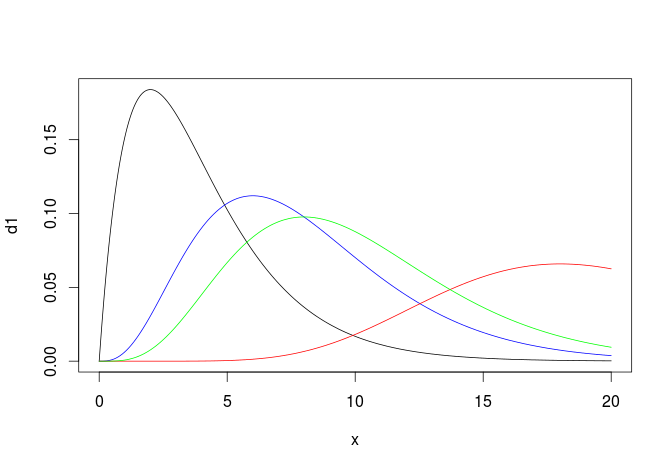
\includegraphics[width=1\textwidth]{Chicuadrado.png}
\label{Ejercicio 4}
\end{center}

\spart
Vamos a usar el resultado visto en clase:
Si $X\sim \gamma(a,p)$ entonces tenemos que 
\[cX \sim \gamma(c\cdot a, p)\]

En este caso, tomando $c=10$ tenemos:

\[\mathbb{P}\{10X\leq 30\} = \mathbb{P}\{\chi^2_{20 }\leq 30\}  \]

Tenemos varias opciontes. Una de ellas es ir a R y calcularlo con el comando \emph{pchisq(30,20)} = 0.93

Y la otra es irse a las tablas y vemos que $\mathbb{P}\{\chi^2_{20} \leq 30\} \simeq 0.93$

\spart Sea $Y \sim \chi_{200}^2$ 

Podemos hacerlo en R directamente y nos da $\mathbb{P}\{Y\leq 3\} = 10 ^{-141}$

A mano, aplicamos el T.C.L, que dice:
\[\sqrt{n}(\gor{X} - \mu) \convs[d] N(0,\sigma)  \]

Entonces tenemos: $\gor{X} \sim N\left(\esp{X},\displaystyle \sqrt{\frac{\var{X}}{n}}\right)$

Donde $\esp{X} = \esp{Z^2} = \var{Z} = 1$ y $\var{X} = \var{Z^2} = \var{\chi_1^2} = 2$

Con lo que:
\[\gor{X} \sim N\left(1,\frac{1}{10}\right)\]

Sustituyendo y estandarizando:

\[
\mathbb{P}\{\gor{X}\leq\frac{3}{20} \} \simeq \mathbb{P} \{Z\leq \frac{\frac{3}{200} - 1}{\frac{1}{10}} \} = \mathbb{P} \{Z\leq -9.85\} = 3 \cdot 10^{-23}
\]

Una diferencia bastante distinta a lo que decía R. Tras un debate entre Miguel y Amparo de 10 minutos no se ha llegado a ninguna conclusión.
\end{problem}

\begin{problem}[4]
\ppart Utilizando el fichero Datos-lipidos.txt, estima, mediante un intervalo de confianza de nivel
0.95, la proporción de pacientes que tienen una concentración de colesterol superior o igual a
220 mg/dl. ¿Qué tamaço muestral habrá que usar para tener una probabilidad aproximada de 0.95 de no cometer un error mayor que 0.01 en la estimación de esta proporción?

\ppart
\solution
Solucionado por Amprao, descargable 
\href{http://www.uam.es/personal_pdi/ciencias/abaillo/MatEstI/T4DatosLipidos.pdf}{aqui}
\end{problem}
\begin{problem}[5] Sea una v.a. con función de densidad $f(x;\theta) = \theta x^{-(\theta) + 1}\ind_{[1,\infty)} $

\ppart Obtener el e.m.v.

\ppart Obtener su distribución asintótica

\ppart Calcular la cantidad pivotal aproximada y, a partir de ella, un intervalo de confianza de nivel aproximada $1-\alpha$ para $\theta$
\solution
\spart \[\dpa{logL(\theta)}{\theta} = 0 \implies e.m.v.(\theta) = \frac{1}{\gor{Y}}\]
donde $Y = log X_i$

\spart Posibles caminos:

a) $\hat{\theta} \convs[d] $¿?

b) \[\sqrt{n}(\hat{\theta} - \theta) \convs[d] N\left(0,?\right)\]

La primera opción es algo difusa y la segunda es mucho más concreta y mejor.

Tenemos que examinar la expresión $\sqrt{n}(\hat{\theta} - \theta)$
Tenemos 2 posibilidades con las que calcular este tipo de cosas (T.C.L) y método delta (que es el que emplearemos a continuación)

\[\mu = \esp{X}; \sigma = \var{X}\]
\[\sqrt{n}\left(g(\gor{X}) - g(u)\right) \convs N(0,\abs{g'(u)} \sigma\]

Aplicando el método delta:

\[
\sqrt{n}(\hat{\theta} - \theta) = \sqrt{ n}\left(g(\gor{y})-g(\esp{Y})\right)\convs[d] N\left(0,\underbrace{\abs{g'\left(\frac{1}{\theta}\right)}}_{\theta^2} \sqrt{\var{Y}}\right) = N(0,\theta)
\]

Peeero... hay que tener cuidado con que $\theta = g(\esp{Y})$ porque sino no podemos aplicar el método delta.

\[
\var{Y} = \esp{Y^2} - \esp{^2 Y} = \underbrace{\int_1^2 (log\,x)^2 \theta x^{-(\theta + 1)}dx}_{\displaystyle\frac{2}{\theta}} - \frac{1}{\theta^2} = \theta{1}{\theta^2}
\]

\spart
La cantidad pivotal les un estadístico que depende de la muestra y del parámetro desconocido (del que estamos calculando el intervalo) y cuya distribución, al menos asintóticamente) es totalmente conocida.

En el apartado b) hemos encontrado la distribución asintótica para poder construir la cantidad pivotal.

Tipificamos el resultado anterior para evitar que la distribución depende del parámetro desconocido.

\[
\frac{1}{\theta} \sqrt{n}(\hat{\theta} - \theta)  = 
\sqrt{n} \left(\frac{\hat{\theta}}{\theta} - 1 \right) = \mathbb{Q}(\theta;X_1,...,X_N)
\]

Esta es nuestra cantidad pivotal, que depende de la muestra (por el $\hat{\theta}$) y depende del parámetro.

\[1-\alpha  = \mathbb{P} = \{q_1(\alpha) \leq \mathbb{Q}(\theta;X_1,...,X_N) \leq q_2 (\alpha)\}\]


El despejar se deja como ejercicio para el lector.

\end{problem}

\begin{problem}[6]
Sea $\sample$ una muestra de una v.a. uniforme en el interalo $[0,θ]$ con $0 < θ < 1$. Obtener una cantidad pivotal para $θ$ a partir del emv. Usando esta cantidad pivotal construye un intervalo de confianza para $θ$ de nivel prefijado $1-α$.

\solution

El e.m.v es \[ emv (θ) = \hat{θ} = \max X_i \] La cantidad pivotal para $θ = Q(θ; \sample)$

\[ F_{X_{(n)}} (x) = \prob{\hat{θ}_n ≤ x} = \prob{X_{(n)} ≤ x} = \prod_{i=1}^{n} \prob{X_i ≤ x} = \begin{cases}
0& x<0 \\
\left( \frac{x}{θ} \right)^n & 0≤x≤θ \\
1 & x > 1
\end{cases}\]

Tomo $Q(θ; \sample ) = \dfrac{X_{(n)}}{θ} = \dfrac{\hat{\theta}}{n}$, que es válido como cantidad pivotal porque \[ \prob{Q≤x} = \prob{\frac{X_{(n)}}{θ} ≤ x} = \begin{cases}
0 & x<0 \\
x^n & 0≤x≤θ \\
1 & x > 1
\end{cases} \]

Tenemos que elegir dos valores $q_1, q_2$ de tal forma que 

\[ 1- α = \prob{q_1(α) ≤ Q(θ;\sample) ≤ q_2(α)} \]

¿Cómo elegirlos? Queremos buscar que la longitud del intervalo de confianza $IC_{1-α}(θ) = \left(\dfrac{\hat{θ}_n}{q_2},\dfrac{\hat{θ}_n}{q_1}\right)$ sea mínima. Calculamos esa longitud:

\[ \text{len IC} = \hat{θ}_n\left(\frac{1}{q_1}-\frac{1}{q_2}\right)=\hat{θ}_n \left(\frac{q_2-q_1}{q_1q_2}\right) \]

Es decir, tenemos que buscar que $q_1-q_2$ sea más pequeño y además tienen que ser lo mayores posible. Por lo tanto, la elección óptima es 

\[ q_2 = 1,\;q_1=α^{1/n} \]

\end{problem}

\begin{problem}[7] Construye tres intervalos de confianza asintóticos diferentes para el parámetro $λ$ de una distribución de Poisson usando los tres métodos siguientes:

\ppart Utiliza el comportamiento asintótico de la media muestral, estima de forma consistente la varianza y aplica el teorema de Slutsky.

\ppart Igual que el anterior, pero sin estimar la varianza

\ppart Aplicando el método delta para \textit{estabilizar la varianza}, es decir, buscando una función $g$ tal que $\sqrt{n}(g(\avg{X}) - g(λ))\convdist N(0,1)$.

\solution

\spart El TCL (\ref{thmCentral}) nos dice que

\[ \sqrt{n}\frac{\avg{X} - λ}{\sqrt{λ}} \convdist N(0,1) \]

Entonces tenemos que 
\begin{equation}
 1-α = \prob{-z_{α/2}≤\sqrt{n}\frac{\avg{X} - λ}{\sqrt{λ}} ≤ z_{α/2}} \label{eqEj7}
 \end{equation}

Sustituyo $λ$ en el denominador por una estimación consistente $\hat{λ}\convs[P, c.s]λ$:

\[ \sqrt{n}\frac{\avg{X} - λ}{\sqrt{\hat{λ}}} \convdist N(0,1) \]

Como sabemos que $λ=\esp{X}$, tomamos la media muestral como el estimador: $\hat{λ} = \avg{X}$. La convergencia nos queda entonces como


\[ \sqrt{n}\frac{\avg{X} - λ}{\sqrt{\avg{X}}} \convdist N(0,1) \]

y por lo tanto tomamos $ \sqrt{n}\dfrac{\avg{X} - λ}{\sqrt{\avg{X}}}$ como nuestra cantidad pivotal. Despejamos ahora en (\ref{eqEj7}):

\[ \prob{\avg{X} - z_{α/2} \sqrt{\frac{\avg{X}}{n}} 
	≤ λ
	≤ \avg{X} + z_{α/2} \sqrt{\frac{\avg{X}}{n}}}
	\]
	
\spart Partimos de nuevo de (\ref{eqEj7}), pero no tenemos que estimar $λ$. Esta ecuación es equivalente a 

\[ \prob{n\frac{(\avg{X}-λ)^2}{λ} ≤ z_{α/2}^2} \]

De ahí sólo tenemos que despejar $λ$ para hallar nuestro intervalo de confianza.

\spart Tenemos que buscar que se satisfaga la ecuación \[ \sqrt{n}(g(\avg{X}) - g(λ))\convdist N(0,1) \]

Sin embargo, el método delta (\ref{defMetDelta}) nos dice algo distinto:

\[ \sqrt{n}(g(\avg{X}) - g(λ))\convdist N(0,\abs{g'(μ)}\sqrt{\var{X}}) \]

Entonces tenemos que 

\[ \abs{g'(λ)}\sqrt{λ} = 1 \implies g'(λ) = \frac{1}{\sqrt{λ}} \]

e integrando vemos que $g(λ) = 2\sqrt{λ} $.
\end{problem}

\begin{problem}[8]
\ppart Se desea evaluar aproximadamente, por el \textit{método de Montecarlo}, la integral 

\[ p = \int_0^1f(x)\,dx \] 

de una función continua $\appl{f}{[0,1]}{[0,1]}$. Para ello se generan 500 observaciones independientes $(X_i,Y_i)$ con $i=1,\dotsc,500$ con distribución uniforme en el cuadrado $[0,1]×[0,1]$ y se estima $p$ mediante

\[ \hat{p} = \sum_{i=1}^{500} \frac{Z_i}{500} \]

donde la v.a. $Z_i$ vale 1 si $Y_i≤f(X_i)$ y $0$ en caso contrario. ¿Qué distribución tienen las $Z_i$? Suponiendo que, en una muestra concreta hemos obtenido $\sum_{i=1}^{500} z_i = 255$, obtener un intervalo de confianza de nivel $0.99$ para la correspondiente estimación de $p$.

\solution

\spart La v.a. sigue una distribución de Bernoulli, de tal forma que

\begin{equation} \prob{Z=1}=\prob{Y ≤ f(X)} \label{eqEj8} \end{equation}

La distribución de densidad de la v.a. $(X_i, Y_i)$ es 

\[ f(x,y) = \begin{cases}
1 & (x,y) ∈ [0,1]×[0,1] \\
0 & \text{en otro caso}
\end{cases} \]

Aplicando esto en $(\ref{eqEj8})$

\[ \prob{Z=1} = \prob{(X,Y) ∈ \{(x,y)\tq y ≤ f(x) \}} = \int_0^1\int_0^{f(x)} \,dy\,dx = \int_0^1f(x)\,dx = p \]

y llegamos a la forma de estimar la integral que queríamos. 

Vamos a contruir el intervalo de confianza de nuvel $0.99$.

\[IC_{0.99} (p) = \left(\gor{z} \pm Z_{0.005}\sqrt{\frac{\gor{z}(1-\gor{\gz})}{500}}\right) = \left(\hat{p} \pm 2575 \sqrt{\frac{\hat{p}(1-\hat{p})}{500}}) \right) = (0.45\pm 0.057)\]


\spart En este caso sabemos el valor de \[p = \int_0^1 x^2dx = \frac{1}{3}\]
Buscamos un $n$ que cumpla: \[z_{0.005} \sqrt{\frac{\frac{1}{3}\cdot\frac{2}{3}}{n}} \implies n > 14734.72\]

\end{problem}

\begin{problem}[9]
Sea X una v.a. con distribución normal de media $\mu$ y variandza $\theta$. Estamos interesados en la estimación de $\theta$ basados en muestras $X_1,...,X_n$. Si $s^2$ denota la cuasivarianza muestras, calcular $\var{s^2}$ y compararla con la cota de Fréchet-Cramer-Rao obtenida en la relación 3 de problemas.
\solution

Comentarios previos: Sabemos que $s^2$ es un estimador insesgado de \[\var{X} = \frac{1}{n-1} \sum_{i=1}^n (X_i - \gor{X})^2\]

Vamos a calcular $\var{s^2}$

Posibilidades:
\begin{itemize}
\item Aunque es un poco largo\[
\var{s^2} = \esp{s^2}-\left[\esp{s^2}\right]^2
\]

\item Si $X\sim N(\mu,\sigma)$ entonces \[\frac{(n-1)s^2}{\sigma^2} \sim \chi_{n-1}^2\]
\end{itemize}

Vamos a utilizar la segunda opción (es un resultado que pondría una referencia pero no se donde está)

\[
\var{s^2} = \var{\frac{n-1}{\sigma^2}s^2\cdot\frac{\sigma^2}{n-1}} = \frac{\sigma^4}{(n-1)^2} \var{\frac{n-1}{s^2}} s^2 = \frac{\theta^2}{(n-1)^2}2(n-1) = \frac{2\theta^2}{n-1} \]

$s^2$ por lo tanto no es eficiente $\left( \text{porque la Cota de FCR es: } \displaystyle\frac{2\theta}{n}\right)$ Por ser $\theta$ la varianza de una $N(\mu,\sigma)$, de la que nos sabemos de memoria la cota de FCR.


\end{problem}

\section{Tema 5 - Contraste de hipótesis}
\subsection{Hoja 5A}

\begin{problem}[1] En octubre de 2007 el periódico \textit{The New York Times} realizó un muestreo en 20 restaurantes y tiendas de Nueva York con objeto de analizar la variable $X$, que representa el contenido en ppm de metilmercurio en el sushi de atún que se pone a la venta. La media y la cuasi-desviación típica muestrales obtenidas con estas 20 observaciones de $X$ fueron $\avg{x} = 0.794,\, s=0.2953$. Supongamos que $X$ tiene distribución aproximadamente normal.

\ppart ¿Proporcionan estos datos suficiente evidencia estadística a nivel $0.05$ a favor de la hipótesis de que la concentración media de metilmercurio en las raciones de sushi de atún en la población considerada es superior a 0.6 ppm? El p-valor, ¿es menor o mayor que 0.01?

\ppart Obtener, a partir de estos datos, un intervalo de confianza de nivel 0.95 para la concentración media de metilmercurio $μ$ en toda la población. Calcular el mínimo tamaño muestral mínimo que habría que utilizar para, con una probabilidad de 0.95, estimar la concentración media de metilmercurio con un error máximo de 0.06 ppm.

\solution

\spart Empezamos definiendo la hipótesis nula, que será que $μ≤0.6$ ya que queremos una evidencia muy fuerte para rechazar que la concentración suba del nivel mínimo.

La región de rechazo en este caso es 

\[ R = \{ T > t_{19;α} \}\]

donde \[ T = \frac{\avg{x} - 0.6}{0.2953/\sqrt{20}} = 2.938 \]

Por otra parte, $t_{19;α} = 1.729$. Se cumple la condición de la región de rechazo, por lo tanto rechazamos $H_0$. El p-valor del contraste tendrá que ser menor entonces que $0.05$.

Para saber si el p-valor es menor que $0.01$ calculamos $t_{19;0.01}=2.53$. Como sigue siendo menor que $T$, seguimos rechazando $H_0$ y por lo tanto el p-valor del contraste será menor que $0.01$.

Si quisiésemos obtener el p-valor concreto del contraste, buscaríamos el valor de $α$ tal que $ t_{19;α} = 2.938$. En R, obtendríamos este valor con la orden

\begin{verbatim}
> pt(2.938, 19, lower.tail=FALSE)
[1] 0.004221168
\end{verbatim}

El p-valor es por lo tanto $0.004$. Esto quiere decir que la probabilidad de obtener la muestra que hemos conseguido suponiendo que $H_0$ es cierta (esto es, suponiendo que la media de ppm de metilmercurio en el atún es menor que $0.6$) es extremadamente baja, y o bien hemos obtenido una muestra muy, muy extraña o $H_0$ es falsa. Por lo tanto, lo razonable sería rechazar la hipótesis nula y decir que, de media, la concentración de metilmercurio media es mayor que $0.6$.

\spart El intervalo de confianza sería 

\[ IC_{0.95} (μ) = \left(\avg{x}\pm t_{n-1;\frac{α}{2}}\frac{s}{\sqrt{n}} \right) = (0.656, 0.932) \]

Como además $0.6\notin IC_{0.95}(μ)$, rechazaríamos $H_0:\,μ=0.06$ a nivel $α=0.05$.

Para hallar el tamñao muestral mínimo buscamos que 

\[ IC_{0.95}(μ) = (\avg{x} \pm 0.06)\]

Despejando, tenemos que resolver

\[ t_{n-1;0.025}\frac{s}{\sqrt{n}} < 0.06\]

Como no conocemos $s$, lo sustituimos por una aproximación, la cuasivarianza muestral de los 20 restaurantes que teníamos al principio. Además, intuimos que $n$ va a ser grande y por lo tanto $t$ se aproximaría a una distribución normal $Z = N(0,1)$, y por lo tanto

\[ t_{n-1;0.025} ≈ z_{0.025} = 1.96 \]

y entonces $n > 93$.
\end{problem}

\begin{problem}[8] 

\ppart Supongamos que en una determinada población de referencia, formada por adultos sanos, el nivel en sangre de la enzima hepática GGT (gamma-glutamil-transpeptidasa) sigue aproximadamente una distribución normal con media polacional $42 IU/L$ y desviación típica poblacional 13. Calcular aproximadamente el porcentaje de personas en la población que tienen un nivel de GGT superior a 80.

\ppart Supongamos ahora que se selecciona una muestra de 61 personas en otra población formada por bebedores habituales no diagnosticados de alcoholismo y se obtiene una media muestra de 58 IU/L con una desviación típica de 21. ¿Hay suficiente evidencia estadística, al nivel 0.05, para afirmar que la concentración media de GGT en la población de bebedores es mayor que 42?

\solution

Sí.

\end{problem}

\begin{problem}[4] Los niveles en sangre de una hormona denominada FSH están asociados con la fertilidad femenina. Las mujeres que tienen un nivel de FSH "alto" (superior a 10 IU/L) tienen en general más dificultad para concebir que aquellas que tienen niveles bajos de FSH. En un estudio realizado recientemente, se analizó la posible relación entre el grupo sanguíneo y la fertilidad. Para ello se midieron los niveles de FSH en una muestra de 254 mujeres en edad fértil con grupo sanguíneo "O" y resultó que 43 de ellas tenían niveles altos de FSH y, por tanto, podrían tener dificultades para concebir. En otra muestra, independiente de la anterior, de 309 mujeres cuyo grupo sanguíneo no es O, resultó que 27 tenían niveles altos de FSH. 

\ppart ¿Proporcionan estos datos suficiente evidencia estadística, al nivel 0.05, a favor de la hipótesis de que las mujeres con grupo sanguíneo 0 tienen más dificultades para concebir que las que tienen otro grupo sanguíneo?

\ppart Calcular el tamaño muestral necesario para, con probabilidad 0.95, estimar en la población de mujeres del grupo 0 el porcentaje de las que tienen un nivel alto de FSH, con un error máximo de 2 puntos.

\solution

Consideramos la v.a. $X$ que vale $1$ si una mujer del grupo 0 tiene nivel alto de FSH y 0 si no, y que sigue una distribución de Bernoulli con probabilidad $p_1$. Análogamente, definimos la v.a. $Y$ que vale $1$ si una mujer del grupo no 0 tiene nivel alto de FSH y 0 si no, y que sigue una distribución de Bernoulli con probabilidad $p_2$.

Tenemos que 

\begin{gather*}
\sum_{i=1}^{254} x_i = 43 \\
\sum_{i=1}^{309} y_i = 27 
\end{gather*}

\spart Primero tenemos que definir la hipótesis nula:

\[ H_0:\: p_1≤p_2 \]

es decir, que las mujeres con grupo 0 no tienen más dificultad para concebir. Tomamos esto como la hipótesis nula porque es la que aceptamos por defecto, y queremos una evidencia muy fuerte para poder decir que es falsa.

Para construir la región de rechazo, usamos la región del formulario para comparación de proporciones. Usando el TCL, tenemos que si $p_1=p_2=p$ entonces tanto $\avg{X}$ como $\avg{Y}$ van a seguir una distribución normal con $n_i = n_1$ o $n_2$ según sea $X$ ó $Y$

\[ N\left(p, \sqrt{\frac{p(1-p)}{n_i}}\right) \]

y por lo tanto el estadístico del contraste es

\[ Z = \frac{\avg{X} - \avg{Y}}{\sqrt{\avg{p}(1-\avg{p})\left(\frac{1}{n_1}+\frac{1}{n_2}\right)}} \]

siendo $\avg{p}$ un estimador puntual de $p$, y que se calcula como 

\[ \avg{p} = \frac{\sum x_i + \sum y_i}{n_1 + n_2} = \frac{n_1\avg{x} + n_2\avg{y}}{n_1 + n_2} \]

La región de rechazo es

\[ R = \left\{ \avg{x} - \avg{y} > z_{0.05}\sqrt{\avg{p}(1-\avg{p})\left(\frac{1}{n_1}+\frac{1}{n_2}\right)} \right\} \equiv \{ 0.0819 > 0.0460 \} \]

y por lo tanto rechazamos la hipótesis nula al nivel $α=0.05$.

Calculamos ahora el p-valor para tener más datos sobre la hipótesis:

\[ \text{p-valor}\, = \prob{N(0,1) > z} = \dotsb \]

\spart Necesitamos un intervalo de confianza

\[ IC_{0.95}(p_1) = \left(\avg{x} \pm z_0.025\sqrt{\frac{\avg{x}(1-\avg{x}}{n_1}}\right) \]

donde $z_0.025\sqrt{\frac{\avg{x}(1-\avg{x}}{n_1}}$ es el error cometido al estimar $p_1$ con el IC, y que tiene que ser menor que $0.02$. Como no tenemos el valor de $\avg{x}$, lo sustituimos por el valor de la media muestral obtenido en la anterior medición, de tal forma que tenemos que $n_1≥1351$ para obtener la confianza requerida. 

Si quisiésemos ser más conservadores, sustiuiríamos $\avg{x}$ por el valor máximo que podemos obtener, aunque en este caso saldría un tamaño muestral mucho más grande.

\end{problem}

\begin{problem}[5] El gasto telefónico medio bimensual en una muestra de 10 usuarios elegidos al azar en una ciudad ha resultado ser 90 euros y la cuasidesviación típica 11 euros. En otra ciudad se ha tomado, de modo independiente, otra muestra de 12 usuarios y los valores obtenidos para la media y la cuasidesviación típica muestrales han sido, respectivamente, 80 y 10.

\ppart ¿Proporcionan estos datos suficiente evidencia estadística, al nivel 0.05, a favor de la hipótesis  de que el gasto medio en la primera ciudad es más alto que el gasto medio en la segunda? Suponer que las varianzas de las variables que indican los gastos telefónicos en ambas ciudades son iguales. Indicar claramente las restantes suposiciones necesarias para garantizar la validez del procedimiento empleado.

\ppart El p-valor ¿es mayor o menor que 0.01? Razonar la respuesta.

\solution

\spart Definimos las dos variables aleatorias que tenemos: $X$ es el gasto medio bimensual en la primera ciudad, y $Y$ el gasto en la segunda. Tomamos las esperanzas y varianzas:

\begin{gather*}
\esp{X} = μ_1,\;\var{X} = σ_1^2 \\
\esp{Y} = μ_2,\;\var{Y} = σ_2^2 
\end{gather*}

 Definimos la hipótesis nula: $H_0:\, μ_1≤μ_2$, es decir, que el gasto medio en la primera ciudad no es mayor que en la segunda.
 
 Tenemos que suponer que $X$ e $Y$ son normales para poder definir bien el estadístico del contraste. Si usásemos cualquier otra distribución el estadístico del contraste toma una distribución mucho más complicada que no podríamos determinar correctamente. También suponemos que son independientes.                       

La región de rechazo es 

\[ R = \left\{ \avg{x} - \avg{y} > t_{n_1+n_2-2, α} s_p\sqrt{\frac{1}{n_1} + \frac{1}{n_2}}\right\} \] 

Calculando, tenmos que 

\begin{gather*}
\avg{x}-\avg{y} = 10\\
s_p^2 = 109.45 \\
R= \{10 > 7.73 \}
\end{gather*}

y por lo tanto rechazamos la hipótesis nula.

\spart Calculamos la región de rechazo para $α=0.01$:

\[ R= \{10 > 11.32 \} \]

y por lo tanto para nivel $0.01$ no hay evidencia para rechazar $H_0$. Entonces, el p-valor es mayor que $0.01$.

\end{problem}

\begin{problem}[6]
Se realiza un experimento para comparar los incrementos en los niveles plasmáticos de insulina producidos por la ingesta de carne y de pescado. PAra ello se midieron los incrementos (medido esn picomoles por litro) producidos en la concentración de insulina en la sangre de 6 voluntarios, 90 minutos después de comer un bistec de 250 gramos. Dos días más tarde se realizó de nuevo el experimento con las mismas 6 personas, después de consumir un filete de pescado. En la tabla se observan los resultados:

\begin{tabular} {|l|c|c|c|c|c|c|}
\hline
Persona & 1 & 2 & 3 & 4 & 5 & 6\\
\hline
Resultados con la carne: & 109& 106 & 111& 105 & 110 & 108\\
\hline
Resultados con el pescado: & 100& 95& 105& 106& 80& 88\\
\hline
\end{tabular}

\ppart Proporcionan estos datos suficiente estadística a nivel significación 0.05 para afirmar que el incremento medio...?
\solution

\spart 

\paragraph{1)} Definir las variables:
\begin{itemize}
\item $X$ nivel de insulina en 1 voluntario tras la ingesta de carne. Llamamos a $\esp{X} = \mu_1$
\item $Y$ nivel de insulina en \textbf{el mismo} voluntario tras la ingesta de carne. $\esp{Y} = \mu_2$
\end{itemize}

Tenemos que las variables no son independientes (porque son muestras tomadas de los mismo voluntarios). A este tipo de datos le llamamos datos emparejados \index{Datos \IS emparejados}

\paragraph{2) Definir las hipótesis}
\begin{itemize}
\item $H_0: \mu_1 \leq \mu_2$
\item $H_1 : \mu_1>\mu_2$
\end{itemize}

\paragraph{3)} Como tenemos datos emparejados, podemos trabajar más facilmente con la diferencia, es decir, definimos $D=X-Y$ y definimos el contraste (siendo $\esp{D}=\mu$)
\begin{itemize}
\item $\Huge_0 : \mu \leq 0$
\item $H_1: \mu >0$
\end{itemize}

Que es un contraste equivalente.

Además tenemos que $D \sim N(\mu,\sigma)$ 

Suponer que la diferencia es una normal es el procedimiento estándar para datos emparejados. (nos la jugamos, es una hipótesis del problema, que puede ser más o menos razonable. En este caso, lo único que de momento sabemos hacer es suponer que es normal (si no fuera normal, tendríamos que aplciar el TCL (para lo que necesitamos n grande) y con este tamaño muestral (6) no podríamos aplicarlo)

Mirando en la tabla de regiones de rechazo tenemos:
\[R = \left\{\gor{d}> t_{n-1;\alpha} \frac{s_d}{\sqrt{n}}\right\}\]
Donde $\displaystyle \frac{\gor{d}}{s_d/\sqrt{n}}$ es el estadístico del contraste, que sigue una $t_{n-1}$.

De los datos extraemos $\gor{d} = 12.5;s_d=10.97$.

Para $\alpha = 0.05$ calculamos el cualtil correspondiente de la $t$ de Student. Para $\alpha = 0.05$ es 9.02.

De aquí deducimos que sí hay evidencia para rechazar la hipótesis nula (porque  $\displaystyle \frac{\gor{d}}{s_d/\sqrt{n}} > 9.02$).

\spart Tomando $\alpha = 0.01$ no se cumple la condición de rechazo, no pudiendo negar entonces la hipótesis nula.

\spart Es el típico ejercicio mecánico de extraer el tamaño muestral.
\end{problem}

\subsection{Hoja 5B}

\begin{problem}[1] Tenemos una $X \sim \mop{exp}(\theta)$. Queremos contrastar para $\alpha = 0.01$ las dos siguientes hipótesis: $H_0: \theta = 5$ frente a $H_1: \theta = \theta_1$, siendo $\theta_1 > 5$ un valor prefijado.

\ppart Obtener la región crítica del test UMP.

\ppart Calcular la probabilidad de error de tipo II en este test.

\ppart Supongamos que para una determinada muestra, se obtiene $\sum_{i=1}^5 x_i= 5$. ¿Qué decisión habría que adoptar si se utiliza el test construido en a)?
\solution

\spart Ejemplo típico de aplicar el lema de Pearson. Primero comprobamos la propiedad de CVM:

\[\frac{f_n(\sample[x];θ_1)}{f_n(\sample[x];5)} = \left(\frac{θ_1}{5}\right)^n e^{-(θ_1-5)\sum x_i} \]

Efectivamente, la función es monótona.

La región de rechazo del test UMP es, por el lema de Neyman-Pearson (\ref{thmNeymanPearson}), la siguiente:

\[ R^{\ast} = \left\{ \left(\frac{\theta_1}{5}\right)^n e^{(-\theta_1-5)\sum x_i > k_α}\right\}
	 = \left\{\sum x_i < c_{\alpha}\right\} \]
	 
¿Cómo construimos $c_{\alpha}$? Tiene que cumplir $\prob[\theta=5]{\sum x_i < c_{\alpha}} = \alpha$

Como $X$ es una exponencial, tenemos que 

\[ \sum X_i \sim γ(θ;n) \]

y entonces

\[ \prob[θ=5]{R}= \prob{γ(5;n) < c_α} \]

De esta forma, $c_α$ es el cuantil $α$ de la distribución Gamma $γ(5;n)$:

\[ c_α = q_{5,n}(α) \]

\spart Calculamos el error de tipo dos, la probabilidad de aceptar la hipótesis nula cuando es falsa:

\[ \prob[θ_1]{R^c}=1-\prob[θ_1]{R} = 1- \prob[θ_1]{\sum X_1 < q_{5,n}(0,01)} = 1 - \prob{γ(θ_1;n)<q_{5,n}(0,01)} \]

Usando las propiedades de la distribución gamma, tenemos que

\[ γ(θ_1;n) = γ\left(\frac{θ_1}{5}5;n\right) = \frac{5}{θ_1}γ(5;n) \]

y entonces

\[ \prob[θ_1]{R^c} = 1 - \prob{γ(5;n) < \frac{θ_1}{5}q_{5,n}(0,01)}
 	= \prob{γ(5;n)≥ \frac{θ_1}{5}q_{5,n} (0,01)} \] 
 	
Este valor tiende a 0 cuando $θ_1\to∞$.

\spart Nuestra muestra nos da una estimación puntual de $\avg{x} = 1$. Bajo la hipótesis nula, la media de la población nos debería de dar $\frac{1}{5}$. Bajo la hipótesis alternativa, la media debería ser estrictamente menor que $\frac{1}{5}$.

Entonces, hay más evidencia a favor de la hipótesis nula así que esperaríamos aceptarla. Comprobémoslo ahora calculando la región de rechazo.

Tenemos que calcular el cuantil de la distribución Gamma:

\[ q_{5,5}(0.01) = 0.2558 \]

No se satisface la condición de la región de rechazo y por lo tanto no hay evidencia para rechazar la hipótesis nula, tal y como habíamos intuido.
\end{problem}

\begin{problem}[3]
El error que se comete en la medición de una magnitud es una v.a. $X$ cuya función de densidad es 

\[ f(x;θ) = \frac{1}{\sqrt{2πθ}}e^{-\frac{x^2}{2θ}} \]

siendo $θ>0$ un parámetro que se desea estimar. Obtener el test uniformemente más potente de nivel $α$ para contrastar $H_0:\,θ≤θ_0$ frente a $H_1:\,θ$

\solution Tenemos que comprobar primero que el cociente de verosimilitudes es monótono. Para ello cogemos dos valores ya ordenados y calculamos la razón de verosimilitudes:

\[ \frac{f(\sample[x];θ_2)}{f(\sample[x];θ_1)} = \left(\frac{θ_1}{θ_2}\right)^{\frac{n}{2}} e^{-\frac{1}{2}\left(\frac{1}{θ_2}-\frac{1}{θ_1}\right)\sum x_i^2} \]

que sí es una función creciente de $T_n=\sum x_i^2$. Por lo tanto esta es una familia paramétrica CVM (ver definición \ref{defFamCVM}). Aplicando el teorema (\ref{thmNeymanPearson2})

\[ R = \{ T_n > k_α \} \tq \prob[θ_0]{R} = α \] 

¿Cómo resolvemos la expresión de $k_α$?

\[ k_α=θχ_{n;α}^2 \]

\end{problem}

\begin{problem}[5] Sea $X_1,\dotsc, X_{16}$ una muestra de tamaño 16 de una población normal de esperanza $μ$ y varianza $σ^2=1$. Se desea contrastar $H_0:\,μ=0$ frente a $H_1:\,μ≠0$.

\ppart Calcula la región crítica del contraste de razón de verosimilitudes de nivel $α=0.05$. ¿Qué decisión se toma a nivel $α=0.05$ si con 16 datos se ha obtenido una media muestra $\avg{x}=1$?

\ppart Para el contraste anterior, ¿cuál es el valor de la función de potencia evaluada en $μ=0.75$?
\solution

\spart
Calculamos la función de verosimilitud:

\[ f(\sample[x];μ) = \frac{1}{(2π)^{n/2}} e^{-\frac{1}{2}\sum(x_i-μ)^2} \]

Nuestro espacio paramétrico es 
\begin{gather*}
Θ_0 = \{ μ=0 \} \\
Θ = ℝ 
\end{gather*}

Entonces el cociente es 

\[ Λ_n = \frac{f(\sample[x];0)}{f(\sample[x];\avg{x}}
 = e^{-\frac{1}{2}\left(\sum x_i^2 - \sum(x_i-\avg{x})^2\right)} = 
e^{-\frac{1}{2}n\avg{x}^2} \]

La región de rechazo es

\[ R=\{ Λ_n < k_α \} \] 

donde $k_α$ es tal que $\prob[μ=0]{R} = α$. La región de rechazo se puede expresar de forma equivalente

\[ R=\{ -2\log Λ_n > c_α\} = \{ n\avg{x}^2> c_α \} \]

con $c_α$ cumpliendo la misma condición que $k_α$. Es decir

\[ α = \prob[μ=0]{n\avg{X}^2 > c_α} \]

Sabemos que la distribución de una media de normales es también una normal: $\avg{X} \sim N\left(0,\frac{1}{\sqrt{n}}\right)$. De la misma forma $\sqrt{n}\avg{X}^2\sim N(0,1)$ y finalmente $n\avg{x}^2\sim χ_1^2$. Entonces

\[ R=\{ n\avg{x}^2 > χ_{1;α}^2 \]

A nivel $α=0.05$, tenemos que \[ R = \{ 15 > 3.84 \], y por lo tanto rechazamos la hipótesis nula.

\spart Tenemos que

\[ β_n(μ=0.75) = \prob[μ=0.75]{\mathrm{rechazar}\,H_0} = \prob[=0.75]{R} = \prob[μ=0.75]{n\avg{X}^2> χ_{1;α}^2} \] 

Evaluando

\[ n\avg{X}^2 = n(\avg{X}-0.75+0.75)^2 = n(\avg{X}-0.75)^2 + 0.75^2 + 2(\avg{X}-0.75)\cdot 0.75 \]

¿Cómo evaluar esta probabilidad? Hacemos algo raro

\end{problem}


\newpage
\chapter{Exámenes}

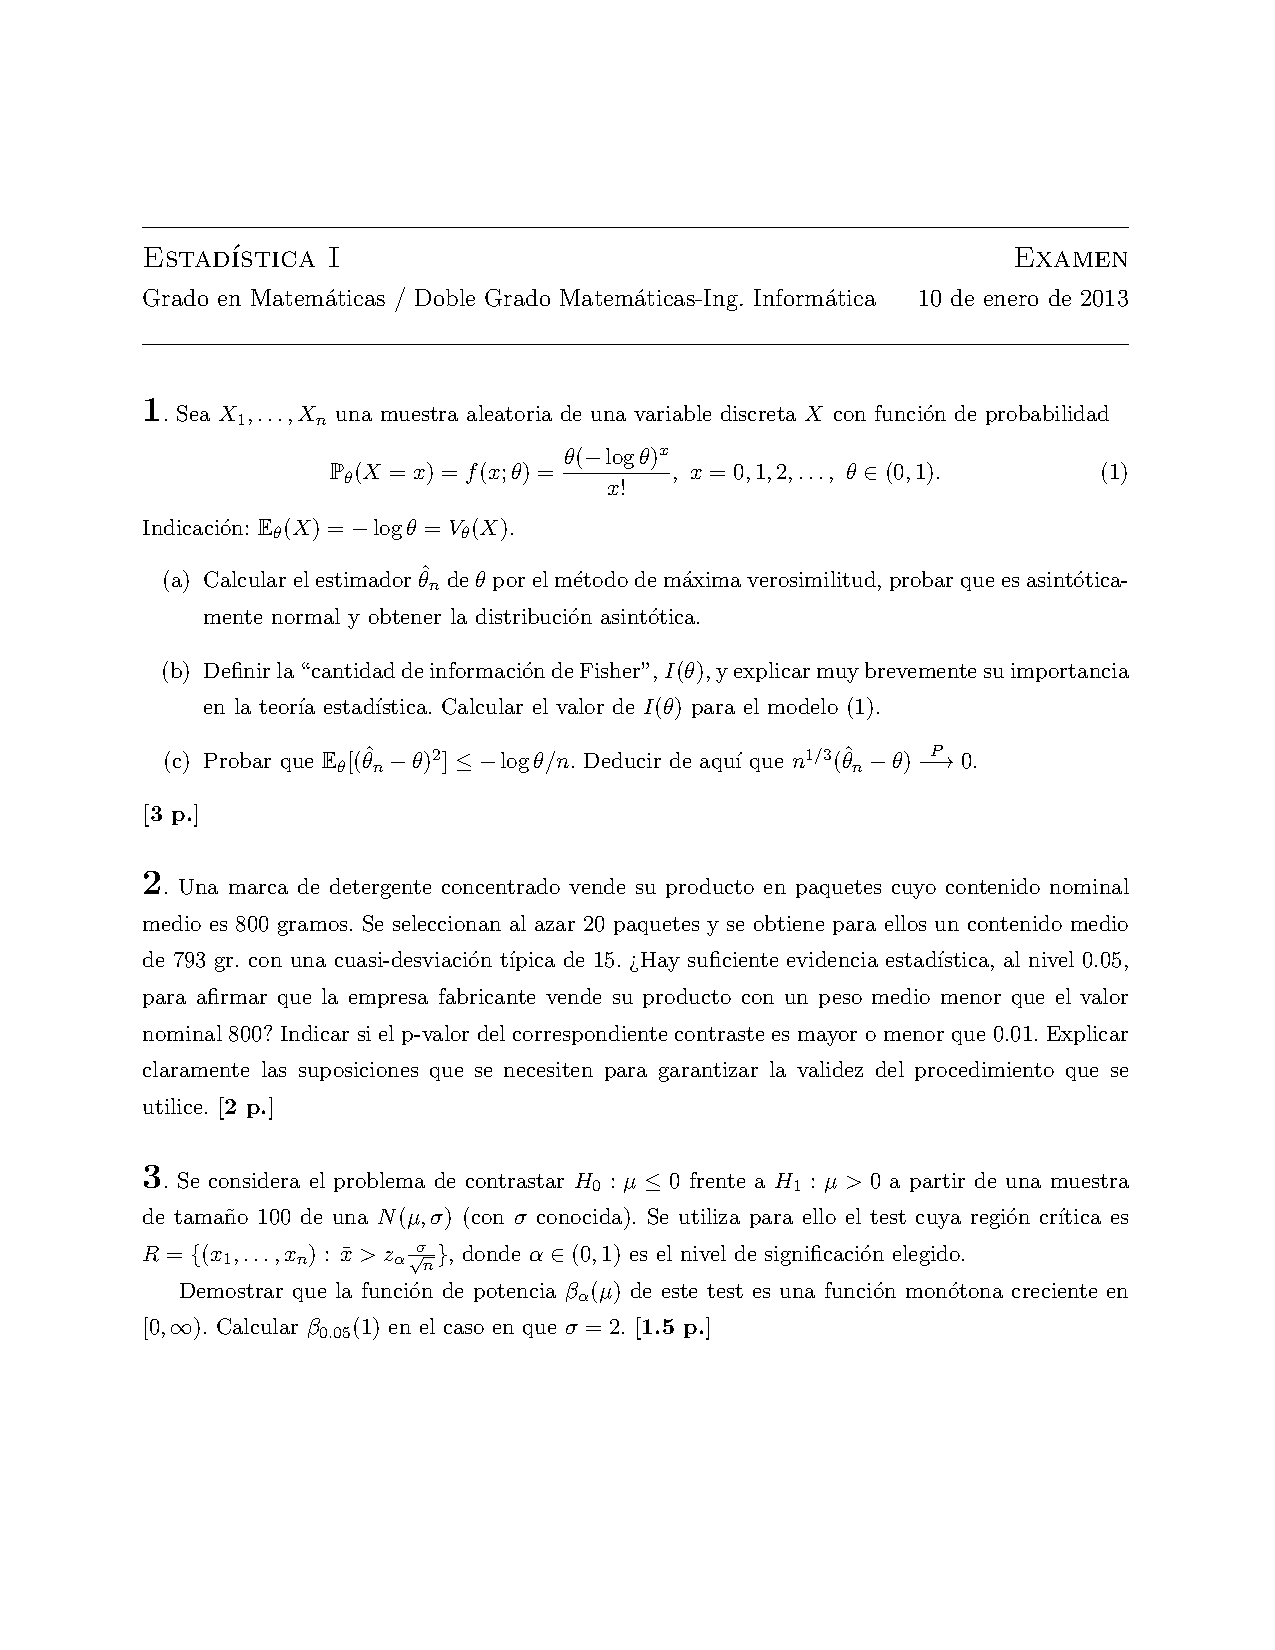
\includepdf[pages=-,addtotoc={1,section,1,Enero 2013,Enero2013}]{pdf/_ExamenEnero2013.pdf}
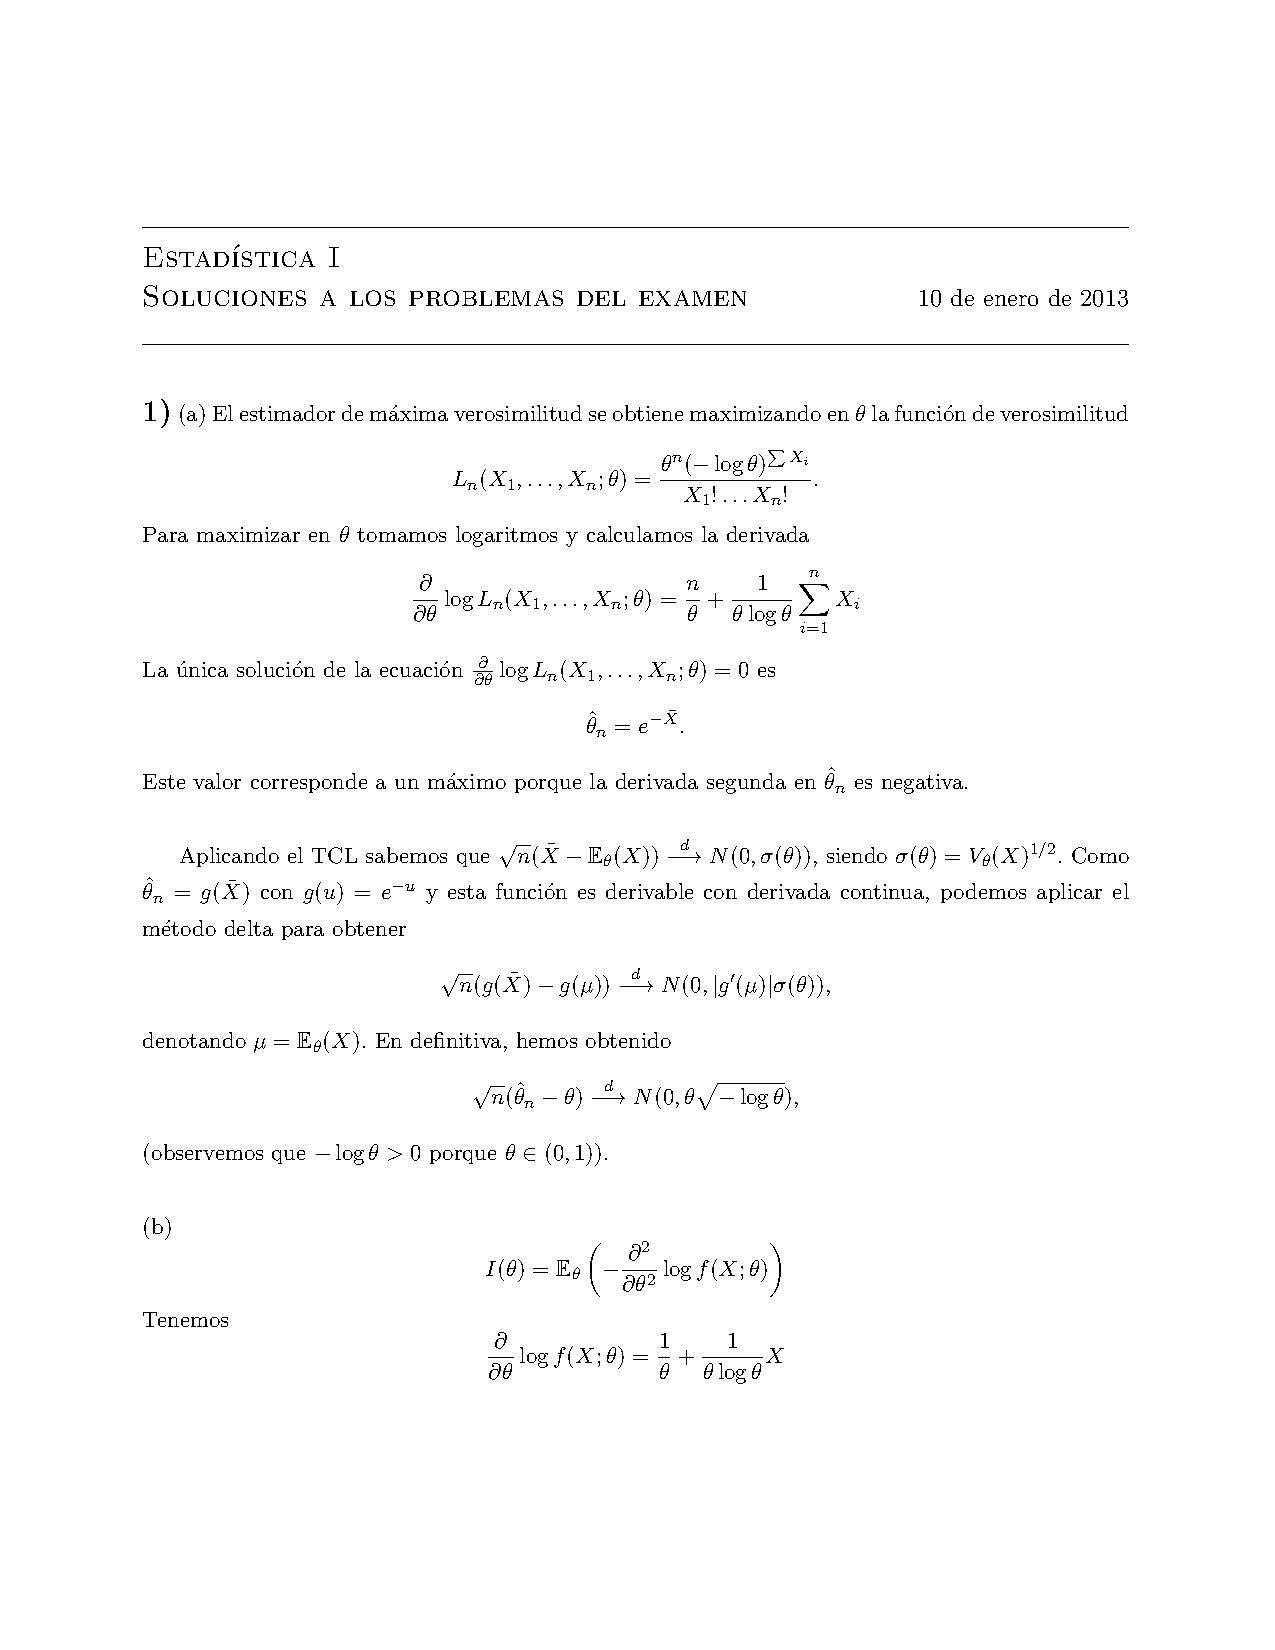
\includepdf[pages=-,addtotoc={1,subsection,1,Solución,Enero2013Sol}]{pdf/_ExamenEnero2013_Sol.pdf}

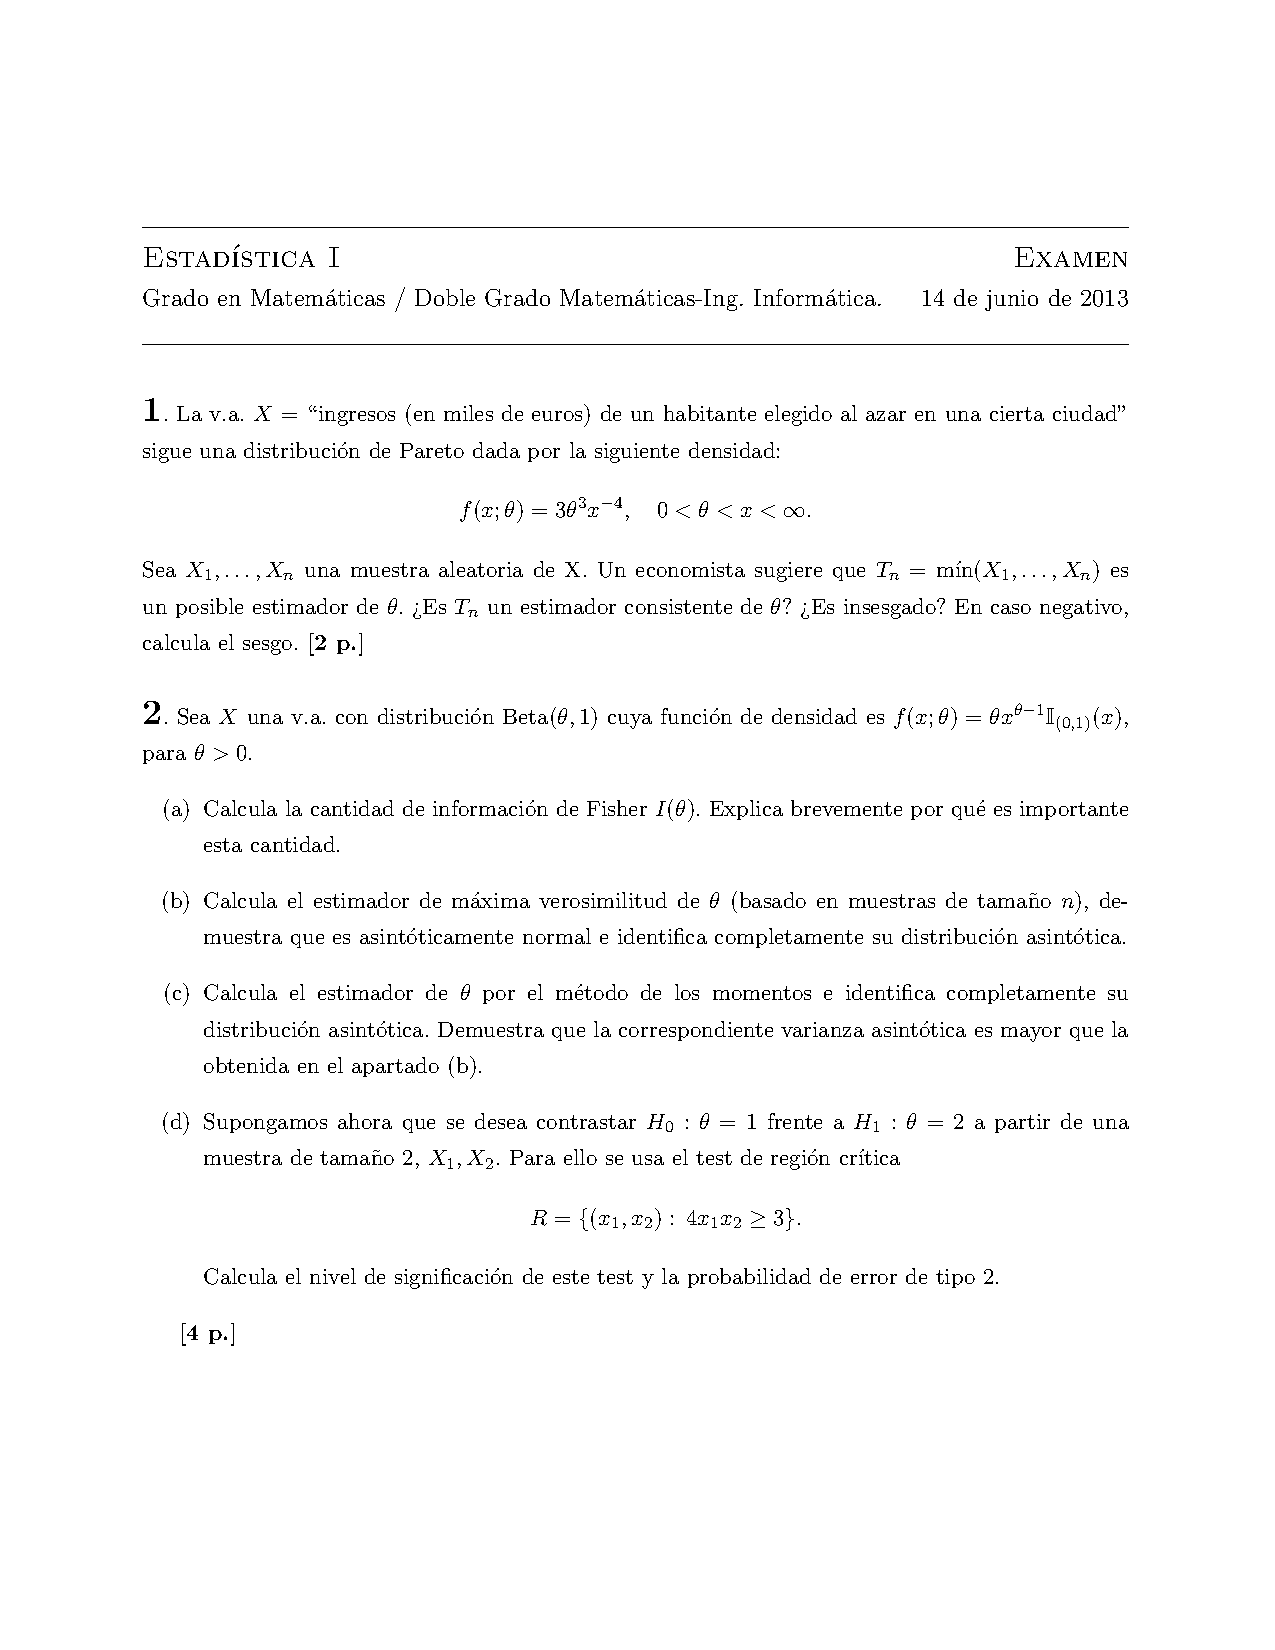
\includepdf[pages=-,addtotoc={1,section,1,Junio 2013,Junio2013}]{pdf/_ExamenJunio2013.pdf}
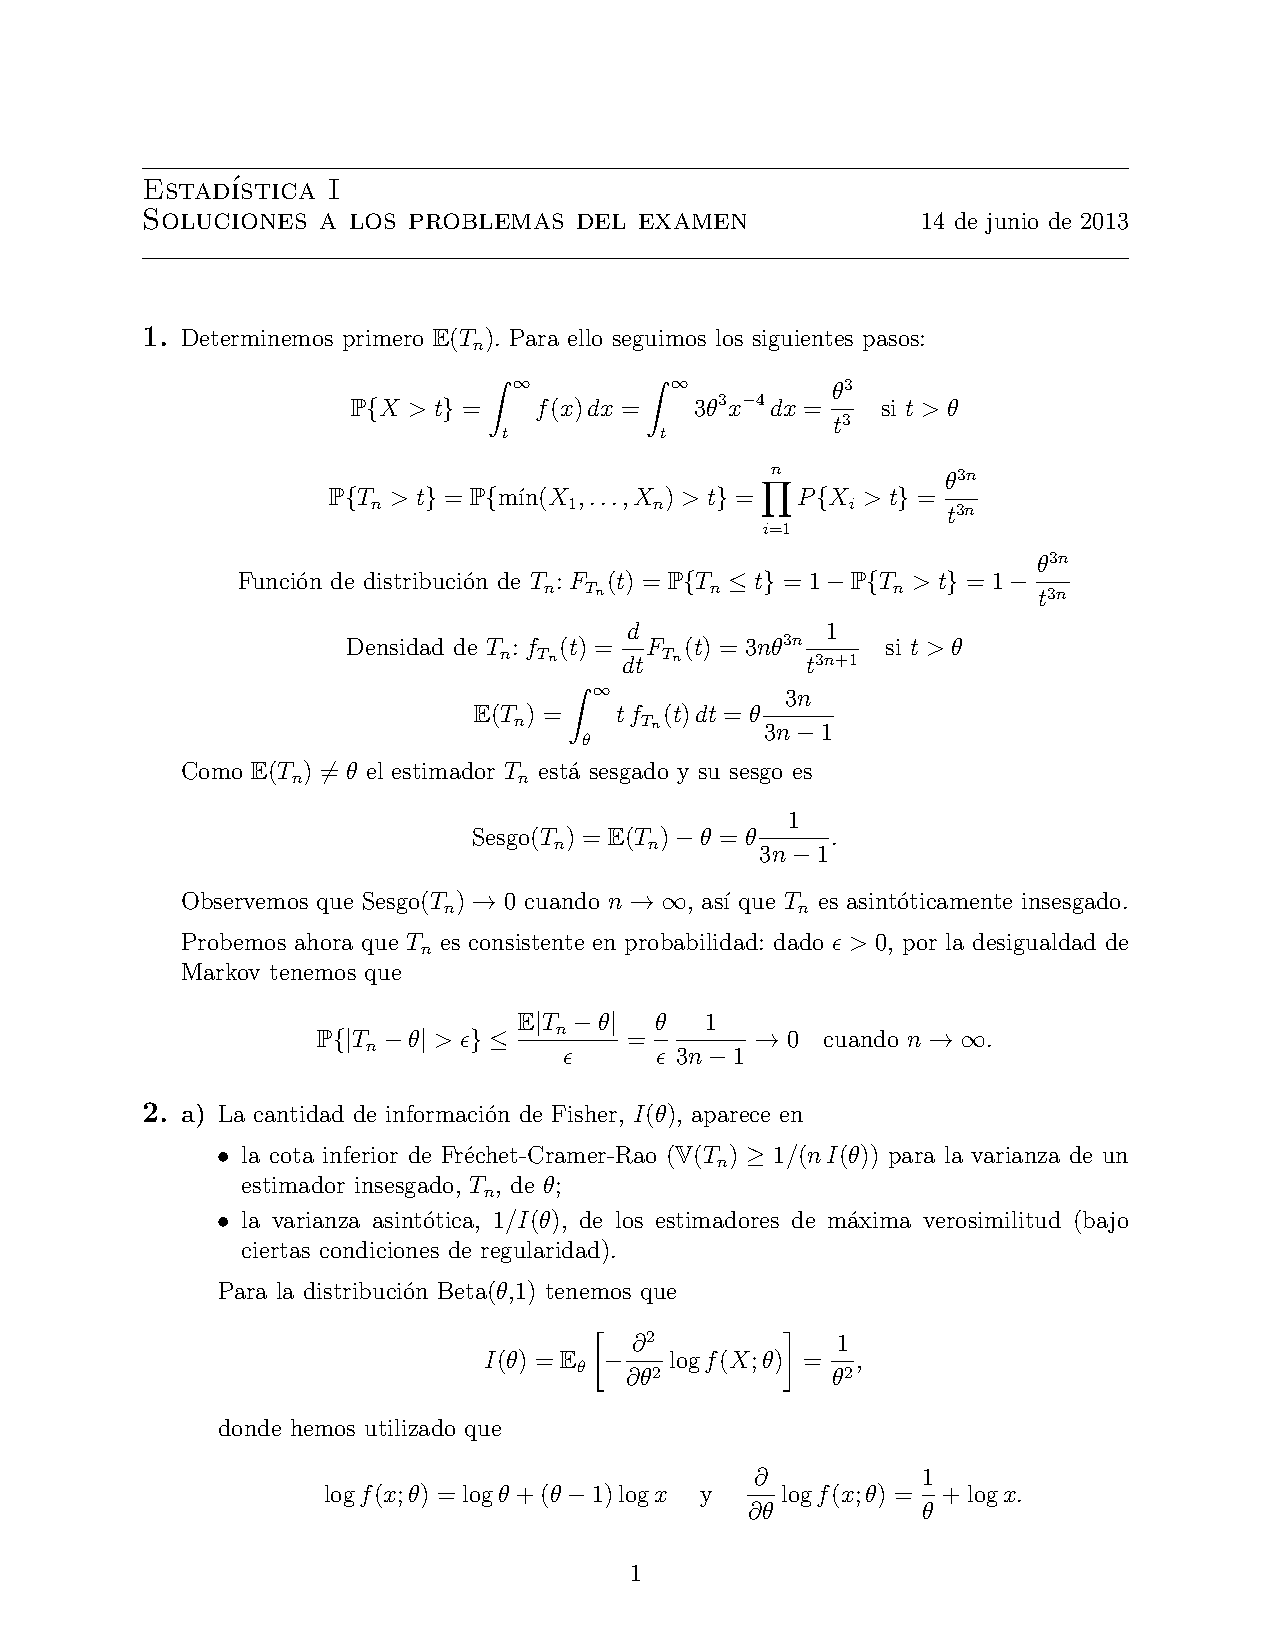
\includepdf[pages=-,addtotoc={1,subsection,1,Solución,Junio2013Sol}]{pdf/_ExamenJunio2013_Sol.pdf}

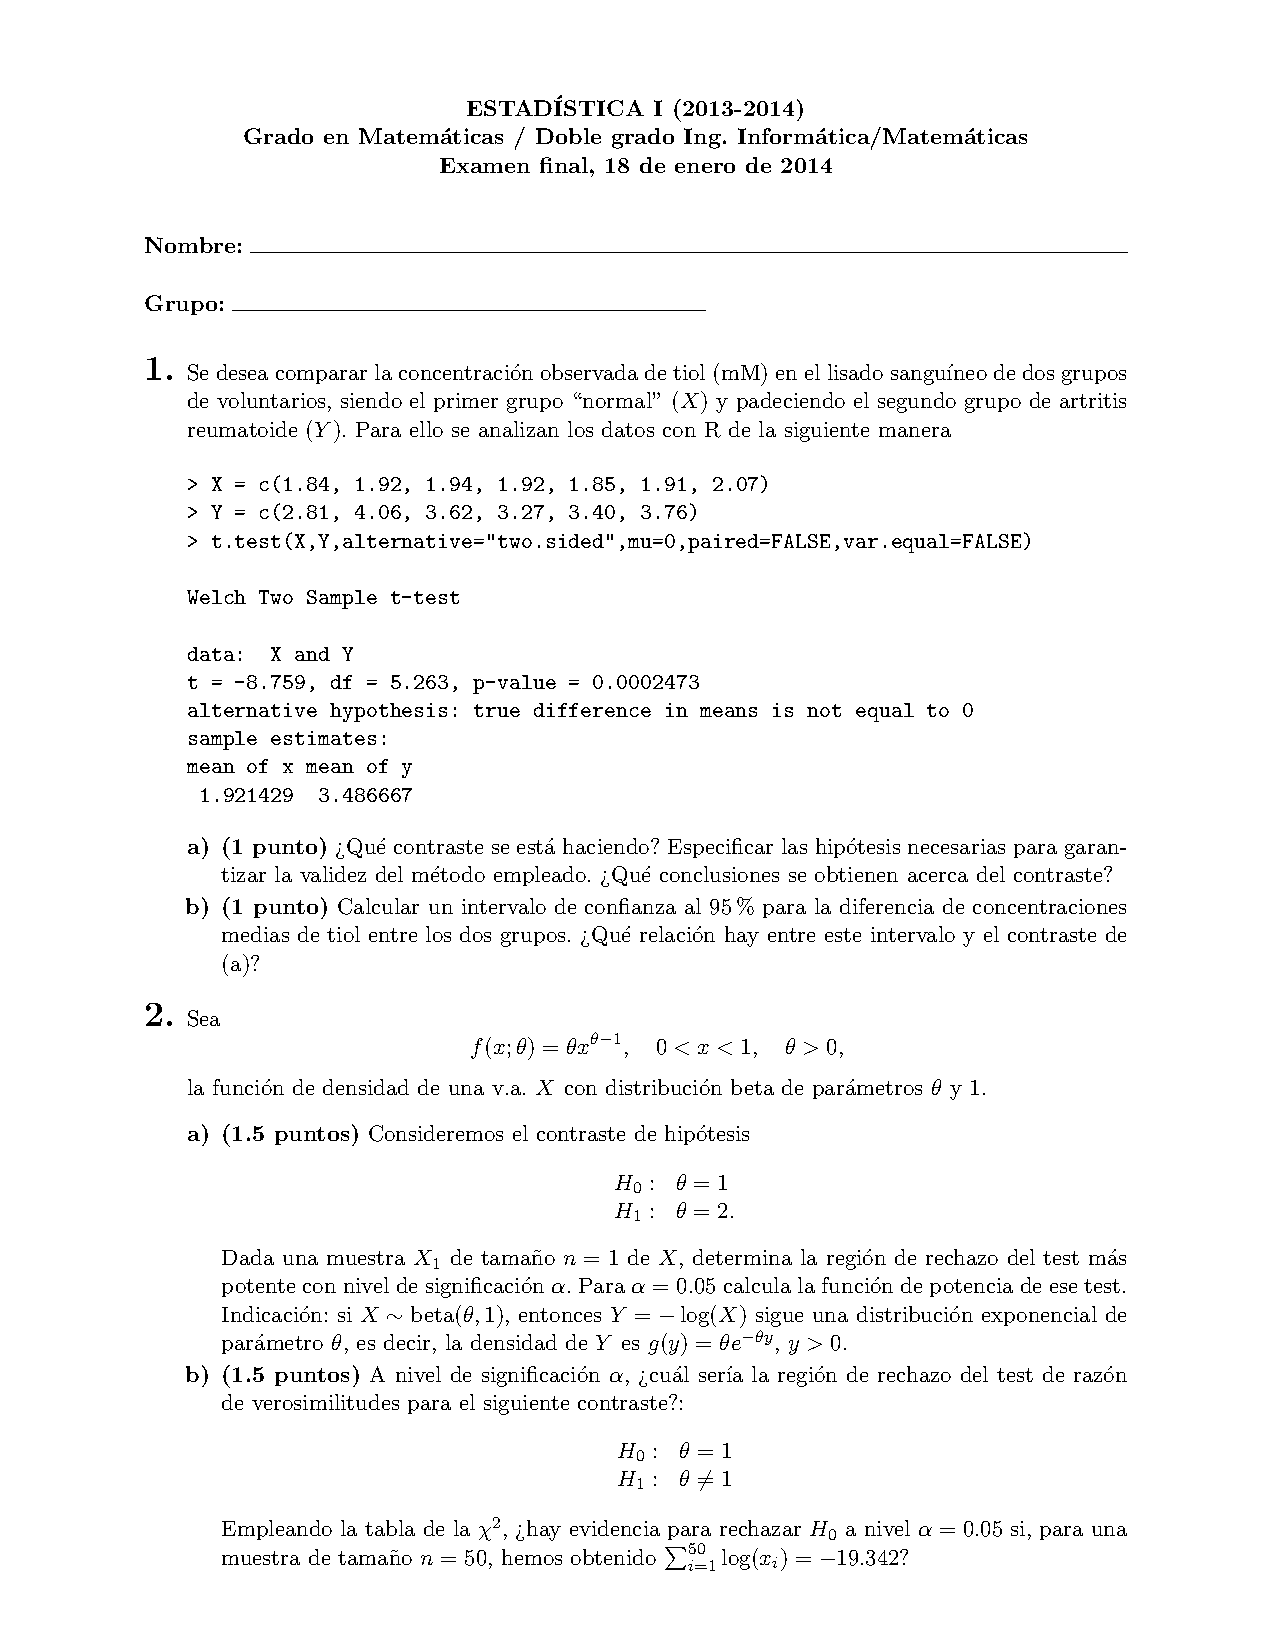
\includepdf[pages=-,addtotoc={1,section,1,Enero 2014,Enero2014}]{pdf/_ExamenEnero2014.pdf}
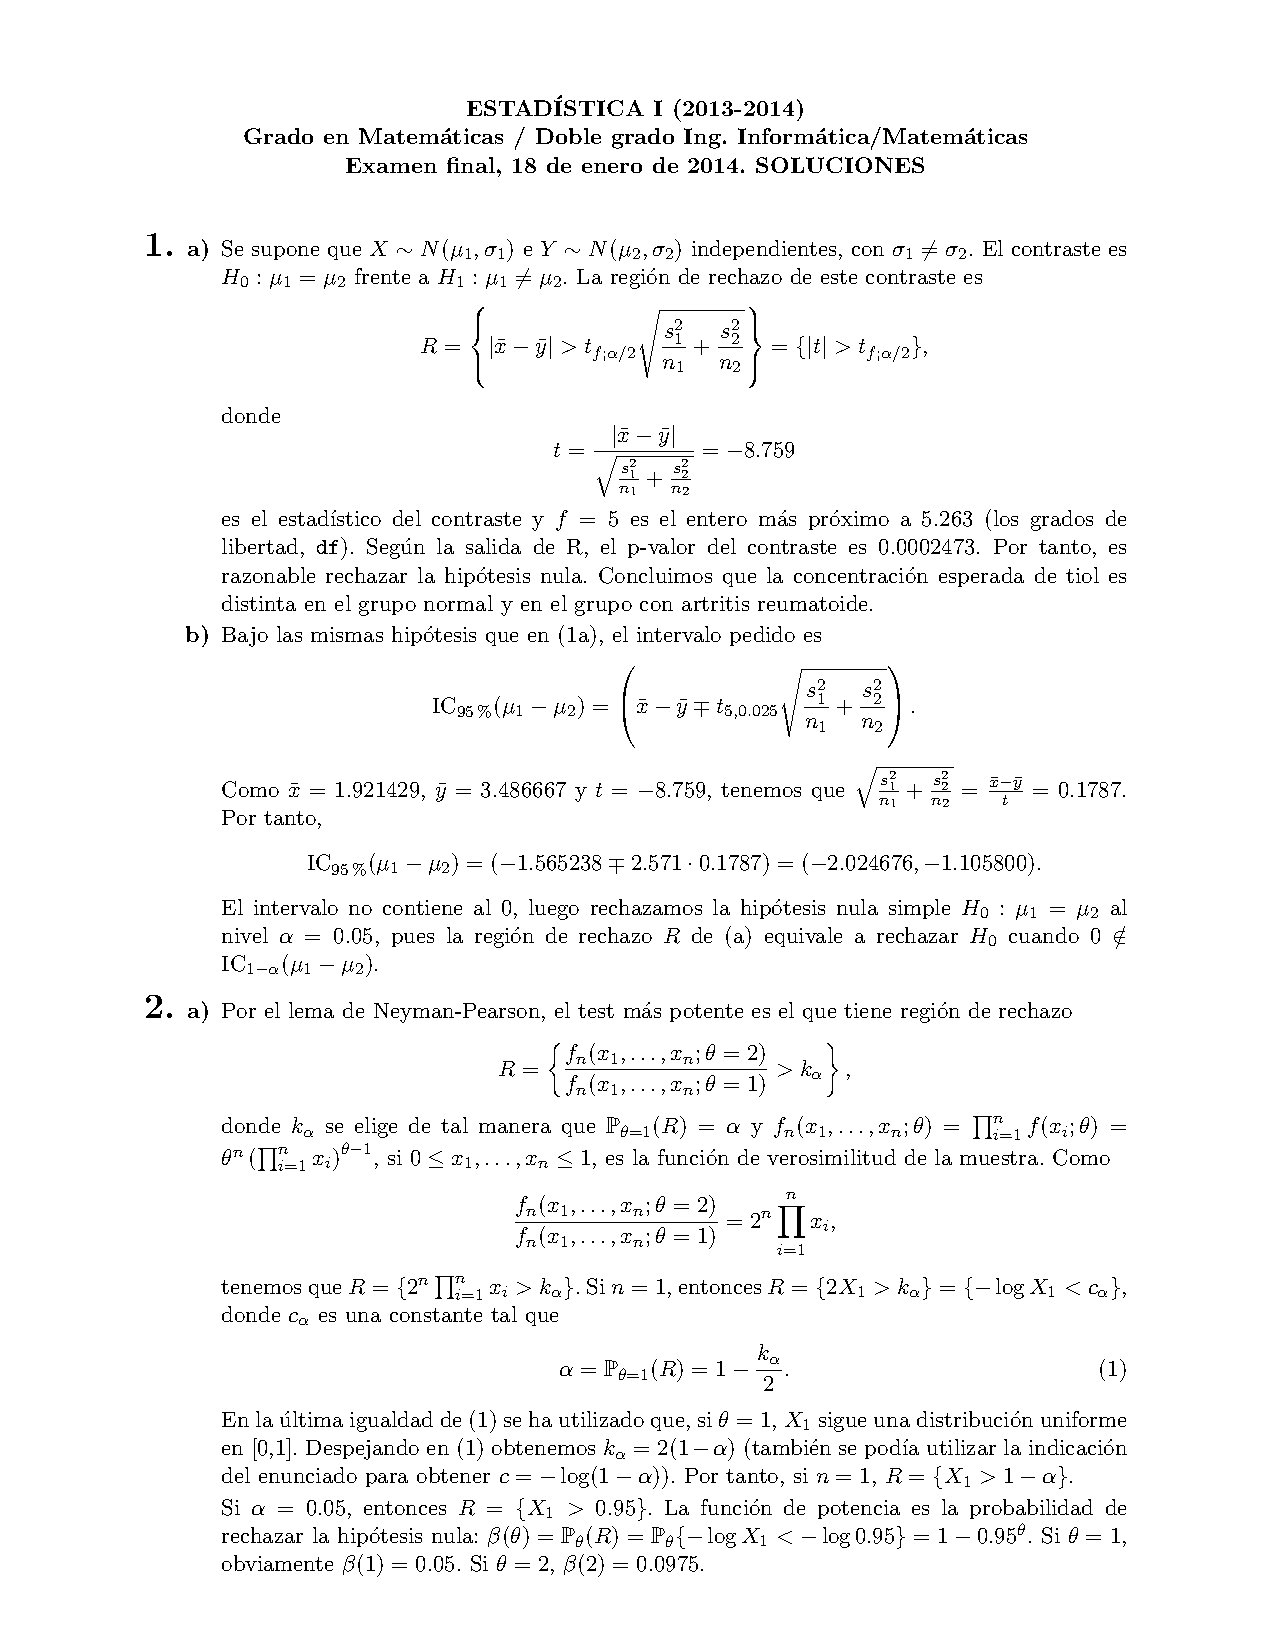
\includepdf[pages=-,addtotoc={1,subsection,1,Solución,Enero2014Sol}]{pdf/_ExamenEnero2014_Sol.pdf}

\printindex


\end{document}

